%& -shell-escape
\documentclass[reqno,12pt,oneside,dvipsnames,svgnames,table,x11names]{report} % 12 point font, print one-sided
\usepackage{pdfpages}  % https://tex.stackexchange.com/a/23776
\usepackage{amsmath}
\usepackage{amsxtra}   % Use various AMS/math packages
\usepackage{amsthm}
\usepackage{amssymb}
\usepackage{amsfonts}
\usepackage{rac}       % Use Rackham style file
% https://texblog.org/2014/12/04/continuous-figuretable-numbering-in-latex/
\usepackage{chngcntr}
%https://www.sharelatex.com/learn/Using_colours_in_LaTeX
\usepackage{xcolor}    % from above document class - https://tex.stackexchange.com/a/83102
\usepackage{paralist}
\usepackage{listings}
\usepackage{caption}
\captionsetup[table]{skip=10pt}
\usepackage{subcaption}
\usepackage{lscape}
\usepackage{tocbasic}
\setuptoc{toc}{totoc}
\usepackage{breakcites}
% https://anjalorenz.wordpress.com/2012/02/14/biblatex-kurz-im-ueberblick/
% https://tex.stackexchange.com/a/134544
% https://www.overleaf.com/help/218-which-bibtex-styles-are-available-on-overleaf
% https://tex.stackexchange.com/questions/34934/add-a-new-empty-page
\usepackage{graphicx}  % Add some packages for figures
\graphicspath{{images/}{custom_fonts/}}
% http://mirror.unl.edu/ctan/macros/latex/contrib/csquotes/csquotes.pdf
\usepackage[autostyle,english = american]{csquotes} 
\usepackage[american]{babel}
\usepackage{verbatim}
\usepackage[bibstyle=apa,citestyle=authoryear-comp,dashed=false,uniquelist=false,uniquename=false,maxcitenames=2,backend=biber,sortcites=false,sorting=nyt,isbn=false]{biblatex}
\DeclareLanguageMapping{american}{american-apa}
\addbibresource{Mley.bib}
\usepackage{rotating}
\usepackage{array}
\usepackage{pdfpages}
% http://www.khirevich.com/latex/microtype/
\usepackage[protrusion=true,expansion=false,final,tracking=false,kerning=false,spacing=false,factor=1100,stretch=5,shrink=5]{microtype}
\usepackage{breakcites}
\usepackage{verbatim} 
\usepackage[printonlyused]{acronym} % For the List of Abbreviations
\usepackage{setspace} % Allows you to specify the line spacing
\usepackage{textcase}
\usepackage{titlesec} % https://tex.stackexchange.com/a/60212
\usepackage{enumitem} % https://tex.stackexchange.com/a/43747
\usepackage{floatrow} % https://tex.stackexchange.com/questions/22751/how-to-force-table-caption-on-top
\floatsetup[table]{capposition=top}
\usepackage[cache=false]{minted}
\usepackage{multicol}
\usepackage{multirow}
\usepackage{longtable}
% https://tex.stackexchange.com/questions/4118/whats-the-quickest-way-to-write-2nd-3rd-etc-in-latex
\usepackage[super]{nth} % 21st, etc.
\usepackage{mathspec}
\usepackage[driverfallback=dvipdfm]{hyperref}
\usepackage[bottom]{footmisc}
\usepackage{marginnote} % side notes
\usepackage{dtk-logos}  % latex logos
\usepackage{xpatch}
\xpatchnameformat{labelname} % GIT, https://tex.stackexchange.com/a/97212
  {\ifciteseen}{\ifnumcomp{\value{listtotal}}{>}{\value{maxnames}}}{}{}
\usepackage{lettrine}
\usepackage[export]{adjustbox}
\usepackage{makecell}

%%%%%%%%% Set manually splitting of words, otherwise may not work properly
\hyphenation{Ma-ni-kas}
\hyphenation{emer-ged}
\hyphenation{re-us-able}
\hyphenation{mod-el-ling}
\hyphenation{ge-ne-ral}
\hyphenation{prob-lem}
\hyphenation{of-fer-ing}

\onehalfspacing           % \onehalfspacing for 1.5 spacing
%%%%%%%%%%%%%%%%%%%%%%
%%%%%%%%%%%%%%%%%%%%%%
%%%%%%% thesis topic -------------- change only here
\newcommand{\MyOwnTopicName}{Discovering Data Science Design Patterns with Examples from R and Python Software Ecosystem}
%%%%%%%%%%%%%%%%%%%%%% 
%%%%%%%%%%%%%%%%%%%%%% Set custom fonts for body text and code
\setmainfont{GaramondPro}[Extension = .ttf, Path = custom_fonts/,UprightFont = *-Regular, BoldFont = *-Bold, ItalicFont = *-It, BoldItalicFont = *-BoldIt]
\setmonofont{SourceCodePro}[Scale=0.90, Extension = .ttf, Path = /usr/share/fonts/opentype/scp/TTF/, UprightFont = *-Regular, BoldFont = *-Bold, ItalicFont = *-It, BoldItalicFont = *-BoldIt] 
%%%%%%%%%%%%%%%%%%%%%%
% https://tex.stackexchange.com/a/69477
\makeatletter                           
\providecommand*{\toclevel@thm}{0}%
\makeatother

% https://tex.stackexchange.com/a/344711
% https://tex.stackexchange.com/a/236657
% https://tex.stackexchange.com/a/26530
\def\UrlBreaks{\do\/\do-}
% https://tex.stackexchange.com/questions/102792/create-table-with-only-header-bold-and-center
\newcommand*{\theadCenterText}[1]{\multicolumn{1}{|c|}{\bfseries #1}}
\urlstyle{same}

% https://www.sharelatex.com/learn/Using_colours_in_LaTeX
\definecolor{quo}{RGB}{110,110,110}
\definecolor{darkor}{RGB}{207, 147, 113}

% qcite macro
\newcommand{\qcite}[1]{\enquote{\emph{\textcolor{quo}{#1}}}}
% patternName macro
\newcommand{\patternName}[1]{\emph{\textcolor{darkor}{#1}}}

\newcommand{\mynameDP}{Dmitrij Petrov}

% current month https://tex.stackexchange.com/a/212264
\newcommand{\monthdataMyOwn}{\ifcase \month \or January\or February\or March\or April\or May \or June\or July\or August\or September\or October\or November\or December\fi\space \number \year}

% https://tex.stackexchange.com/a/10449
\counterwithout{table}{chapter}
\counterwithout{figure}{chapter}
\counterwithout{footnote}{chapter}

% for tables
\newcolumntype{L}[1]{>{\raggedright\let\newline\\\arraybackslash\hspace{0pt}}m{#1}}
\newcolumntype{C}[1]{>{\centering\let\newline\\\arraybackslash\hspace{0pt}}m{#1}}

% https://tex.stackexchange.com/a/406872
\makeatletter
\newcommand{\currentfontsize}{\fontsize{\f@size}{\f@baselineskip}\selectfont}
\makeatother

% https://tex.stackexchange.com/a/35547
\setminted{fontsize=\footnotesize,baselinestretch=1,linenos,breaklines}
\setmintedinline{fontsize=\currentfontsize}

% https://www.sharelatex.com/learn/Hyperlinks#Linking_local_files
% https://tex.stackexchange.com/questions/100905/best-practice-for-hyperref-link-colours
\hypersetup{pdfencoding=auto,colorlinks=true,linkcolor=black,urlcolor=black,citecolor=black, pdfpagelayout=TwoPageLeft,pdfstartpage = 1, pdffitwindow = true,pdfpagemode=UseNone,pdfauthor={\mynameDP},pdftitle={\MyOwnTopicName},breaklinks=true,pdfkeywords={R, python, data science, software ecosystems, design patterns}}
%%%%%%%%%%%%%%%%%%%%%%%%%%%%%%%%%%%%%%%%%%%%%%%%%%%%%%%%%%%%%%%%%%%%%%%%%%%%%%
% If printing two-sided, this makes sure that any blank page at the
% end of a chapter will not have a page number.
\makeatletter
\def\cleardoublepage{\clearpage\if@twoside \ifodd\c@page\else
\hbox{}
\thispagestyle{empty}
\newpage
\if@twocolumn\hbox{}\newpage\fi\fi\fi}
\makeatother

\AtEndPreamble{\usepackage[autoprint=true]{pythontex}}
%%%%%%%%%%%%%%%%%%%%%%%%%%%%%%%%%%%%%%%%%%%%%%%%%%%%%%
%%%%%%%%%%%%%%%%%%%%%%%%% Begins the real document
%%%%%%%%%%%%%%%%%%%%%%%%%%%%%%%%%%%%%%%%%%%%%%%%%%%%%%
\begin{document}
\cleardoublepage

\Coverpage{\MyOwnTopicName}{\mynameDP}

\includepdf[pages={1}]{images/Wi2_Deckblatt_DP_Thesis.pdf}
\cleardoublepage

\titlepage{\MyOwnTopicName}{\mynameDP}{Master of Science}
{International Information Systems}{\monthdataMyOwn\@}
{Prof.\ Dr.\ Freimut Bodendorf, Chair of Institute of Information Systems II, FAU\\
Research Assistant Isabella Eigner, Institute of Information Systems II, FAU\\
Research Assistant Alexander Piazza, Institute of Information Systems II, FAU}{Student ID: 21998127}
\cleardoublepage

% Begin the front matter as required by Rackham dissertation guidelines
\initializefrontsections

\copyrightpage{\mynameDP}

\statutoryDeclaration
\begin{doublespacing}
\newcommand{\textfield}[2]{
  \vbox{
    \hsize=#1
    \kern2.5cm
    \hrule
    \kern0.1ex
    \hbox to \hsize{}
  }
}

\begin{center}
{\large\bf STATUTORY DECLARATION}
\end{center}
Ich versichere, dass ich die Arbeit ohne fremde Hilfe und ohne Benutzung anderer als der angegebenen Quellen angefertigt habe und dass die Arbeit in gleicher oder ähnlicher Form noch keiner anderen Prüfungsbehörde vorgelegen hat und von dieser als Teil einer Prüfungsleistung angenommen wurde. 
Alle Ausführungen, die wörtlich oder sinngemäß übernommen wurden, sind als solche gekennzeichnet.
\newline
\newline
I assure that this thesis is a result of my personal work and that no other than the indicated aids have been used for its completion.
Furthermore, I assure that all quotations and statements that have been inferred literally or in a general manner from published or unpublished writings are marked as such.
Beyond this I assure that the work has not been used, neither completely nor in parts, to pass any previous examination.

\hbox to \hsize {
  {\today} in Nuremberg, Germany
  \hfil
  \hfil
  \textfield{7cm}{Signature}
}
\end{doublespacing}


\dedicationpage{Dedicated to my parents,}{my thesis committee,}{my reader,}{and myself.}

% Page numbering. If you don't include a frontispiece or copyright page, you'll need to change this for two-sided printing.
\makeatletter
\if@twoside \setcounter{page}{4} \else \setcounter{page}{1} \fi
\makeatother

\startacknowledgementspage
\begin{center}
{\large\bf ACKNOWLEDGEMENTS}
\end{center}

First and foremost, I would like to express my very great appreciation to my parents who allowed me to pursue my dreams, in many cases by sacrificing their own.
Hearing their countless advices and having a spiritual and financial support since my childhood, I hope that this graduate thesis will be rewarding to them the same way as it has been to me. 

Even more importantly, I would like to thank Prof.\ Dr.\ Freimut Bodendorf, M. Sc. Isabella Eigner and M. Sc. Alexander Piazza -- my research co-supervisors -- for their academic supervision, guidance, encouragements and critiques of this work.

Additionally, I am very grateful to Dr.\ John Morley of Manchester University in creating the \emph{Academic Phrasebank} -- an invaluable resource for all academicians.

Finally, I owe a debt of gratitude to the scholars at the University of Michigan in the USA who have developed a \LaTeX\ template that I have used, with adjustments, for my dissertation.

\label{Acknowledgements}

\startabstractpage
\begin{singlespace}
\indent \textbf{Background:} A variety of software design patterns in the computer science are documented assisting practitioners to reuse best solutions to commonly occurring problems. 
However, lacking researchers' attention so far, design patterns were not yet formulated for a newly established \emph{data science} field which aims to extract actionable knowledge from data. 

\textbf{Objective:} From the perspective of data scientists and other engineers, the study set out to discover and understand \emph{data science design patterns}.
Consequently, by supplementing such candidates with R and Python code examples utilizing packages from their software ecosystems, the objective was to develop \emph{Data Science R and Python Toolkit Matrix} as well.

\textbf{Method:} Based on the \emph{data-driven design pattern production} methodology, the research first gathered relevant and contemporary source material. 
Later, through a general inductive approach, data were coded resulting into emergence of an exhaustive list of key themes from which a group of pattern candidates was described according to a defined template. 
The purposeful sampling of utilities from \acs{CRAN} and \acs{PyPI} repositories further contributed to developing above mentioned matrix too. 

\textbf{Results:} In this study, ten data science design patterns were formalized and \emph{Data Science Toolkit Matrix} was derived consisting of thirty-two R and Python tools deemed capable of addressing frequently occurring problems faced by practitioners when analysing data large and small. 

\textbf{Limitations:} Thesis' validity might have been hampered by the collection and interpretation of sources on which the study relied on to discover design patterns. 
To mitigate, a workshop with experts from the field could improve patterns' quality and gain their greater validation.
From the perspective of the toolkit matrix, the work focused only on tools for two-dimensional data, and hence omitted technologies for computer vision, all of which should be addressed in the future research.

\textbf{Conclusion:} The thesis has contributed to the study of design patterns by specifically focusing on data science domain while considering relevant R and Python tools from their software ecosystems.
For aspiring data scientists, this work laid out a foundational ground by providing them an overview of best practises for dealing with typical issues in data collection, manipulation and visualization.
As a result of identified design patterns and R and Python utilities, findings also help to better understand what other programming languages such as Julia need to offer and support in order to become widely used for the knowledge discovery purposes.

\bigskip
\noindent \textbf{Key Words:} Software ecosystems, design patterns, data science, R, Python, FOSS, packages

\end{singlespace}
\label{Abstract}

% Table of contents, list of figures, etc.
\tableofcontents     % Required
\listofappendices    % Required if there is more than one appendix
\listoffigures       % Required if there is more than one figure
\listoftables        % Required if there is more than one table
\listoflistings      % for code
\listofabbreviations % Abbreviations should be stored in a file named abbr.tex

\startthechapters
%%%%%%%%%%%%%%%%%%%%%%%%%%% For later in chapter 1
\newcommand{\ObjectivesQOne}{How do scientists understand the concepts of \emph{software ecosystem}, \emph{data science} and \emph{design pattern}?}
\newcommand{\ObjectivesQTwo}{Based on the additionally reviewed literature, which data science-oriented design patterns can be recognized?}
\newcommand{\ObjectivesQThree}{Surveying R and Python \acs{FOSS} ecosystems, what are the specific tools that solve common problems when discovering knowledge from data?}
%%%%%%%%%%%%%%%%%%%%%%%%%%%
\cleardoublepage
\clearpage
\vspace*{\fill}
\hfill
\begin{center}
This page is intentionally left blank.
\end{center}
\vspace{\fill}
\thispagestyle{empty}
\newpage
\clearpage
\cleardoublepage
%%%%%%%%%%%%%%%%%%%%%%%%%%%%
\setcounter{page}{1}
 \chapter{Introduction}
   \label{chap:Intro-Chap1}
   \lettrine[lines=2]{\color{BrickRed}I}{n} the following pages, the reader is introduced to this thesis. 
At the beginning, the subject matter is delineated, followed by laying out the problem statement, objectives, methodology and delimitations of the endeavour.
Finally, document's structure is described too.

\acused{FOSS}
\acused{ETL}
\acused{DS}
\acused{ML}
\acused{BI}
\acused{KDD}
\acused{DSTM}
\acused{SECO}
\acused{GIA}
\acused{IT}
\acused{UI/UX}
\acused{3D2P}
\section{Overview}
\label{motfac}
A term \emph{pattern} embodies a multitude of concepts which can be used in a variety of contexts, for example in nature to describe wavelike shapes on sand dunes in the desert.
Besides its use in the art or in the fashion for decorative purposes, patterns in mathematics are commonly known as \emph{fractals} which are never ending geometric shapes that exhibit the \qcite{same \enquote{type} of structure on all scales} (\emph{self-similarity}; \cite{Fractal2017}). 

From the \emph{knowledge discovery in databases} (\ac{KDD}) perspective, diverse algorithms are applied to uncover \qcite{interesting, [insightful,] unexpected and useful patterns in} data \parencites{PatternMining2013}{Witten2011}{GoebelMichGru1999}. 
In accordance with a \emph{data pyramid}, ultimately turning such information into a wisdom \parencite{Rowley2007TheHierarchy}.
Yet the focus of this study considers the meaning of patterns being first formulated in a book entitled \emph{A Pattern Language} by \textcite{Alexander1977}. 

Since Christopher Alexander's profound publication in the field of architecture, patterns have become a topic of a great interest and have had a large influence in a wide range of areas as well.
Perhaps the most important classical literature work appeared some twenty years later by \textcite[11]{GoF2002} who introduced twenty-three \emph{design patterns} for developing \qcite{reusable object-oriented software} applications.
The authors known as \emph{\ac{GoF}} described their abstract approaches as a \qcite{recurring solution to a standard problem}, essentially concerned with \qcite{a way to solve a specific problem of design} \parencites[37]{Schmidt:1996:SP:236156.236164}{Werner2006}. 

Over\marginnote{Importance of Patterns}, the past four decades, a growing body of research in the computer science has recognised the importance of patterns as useful techniques facilitating for instance better communication and collaboration between engineers and their managers \parencite{Schmidt:1996:SP:236156.236164}.  
Rooted and validated in the practise, they are \qcite{identified and verified through careful observation} providing a reliable, \qcite{orderly resolution of software development problems (\dots) and help new developers ignore traps and pitfalls that have traditionally been learned only by costly experience} \parencites{Werner2006}[37]{Schmidt:1996:SP:236156.236164}.
Therefore, their adoption for \qcite{documenting complex architectural designs} gave them a firm place during the phases of software analysis, design and implementation \parencites[47]{Stefan2017}{Chetan2016}.  

\marginnote{Data Science $\land$ Design Patterns}
Stepping aside for a moment, companies nowadays collect digital information that over time has grown both in volume and its variety.
In order to realize its full potential, in cases like preventing financial fraud, new technologies are used to transform captured data from various internal and external locations with a goal to extract valuable knowledge and gain a wisdom for business operations through data visualizations and storytelling \parencite{NicolausHenke2016TheWorld}.
Thus, eventually, making corporate processes, products and services more data-driven.
However, unfortunately as it has been documented in countless instances, when raw data are translated into actionable insights for employees, reoccurring issues are often faced \parencites{HolleyKerrir2014}{Hossam2017}.

Subsequently, one of the challenges encountered by many researchers, \emph{data scientists} and other \emph{big data} engineers has been how to effectively share among each other best practises and gained experiences to frequently confronted obstacles.
The answer, which has been suggested, involves applying design patterns not only for communication and documentation purposes but also for the entire knowledge management. 
This due to their capability of addressing hurdles efficiently by means of having a narrow scope with defined structure that captures a problem and offers a solution \parencites{Hossam2017}{DeardenHCI2006}. 

\marginnote{Research Gap}
As later shown in the \textbf{chapter \ref{chap:KeyTerms}}, to date, a significant pattern research has been carried out in the education, sociology or in the multidisciplinary field of information technology (\ac{IT}). 
There, patterns have been examined for the enterprise architecture or targeting specific software applications such as \emph{Hadoop} \parencites{Fowler2002}{MinerDonald2012}. 
Surprisingly, however, little research has formally studied design patterns in relation to data science (DS) or machine learning (ML) -- the research gap that is identified and addressed.
Indeed, to the best of author's knowledge, design patterns have been so far undocumented in a broad \ac{DS} domain which is the main focus of this work.

Arguably, one of the reasons has been an ambiguity of such umbrella term \ac{DS} and its dynamic nature which is manifested in the ever-evolving technologies and approaches to business analytics \parencite{CarlShan2015TheScientists}.
Therefore, the goal of this thesis is to systematically discover and describe such general, \qcite{time-tested design solutions} to common problems that appear during the data analysis \parencite[853]{HeffreMheer2006}.  
The significance of this subject matter is also underscored by a forthcoming book entitled \emph{Data Science Design Patterns} by \textcite{Todd2019}.

\marginnote{R $\land$ Python}
To further complement the intended research, in the past decade academicians and practitioners have tried to determine what programming language and its ecosystem is \enquote{more valuable} to learn, \enquote{more powerful} to work with and generally \enquote{better} to use for \ac{KDD} purposes \parencites{DavidMa2016RAdvances}{PeterWayner2017PythonShare}{MartijnTheuwissen2015R}{ChengHanLee2015HowFirst}.
According to different questionnaires, forum discussions and rankings, there seems to be an agreement that two programming languages -- R and Python -- are especially important for \ac{DS} \parencites{Muenchen2017TheSoftware}. 

\marginnote{Intentions}
In this study, firstly, the objective is to devote an attention to the research gap faced by the interdisciplinary talented practitioners when they conduct typical analyses of data. 
Through identifying and describing best practises in a design pattern form and being consistent with authors such as \textcite{DPCPQT2011}, \emph{pattern candidates} are then supplemented with R and Python code examples and tools from their ecosystems. 
These utilities can be chosen by a next generation of quantitative analysts to support their work on data-driven knowledge discoveries \parencite{MosaicDataScience2017}. 
As a result, it also permits to gain a better understanding of what computer programs from two \ac{DS} environments are available to solve domain specific hindrances.

Because the current research has so far lacked surveys of applications from either programming landscape, the second aim of this inquiry is to develop \emph{Data Science R and Python Toolkit Matrix}, henceforth referred to as \ac{DSTM}.
This can be used as a guideline by all interested stakeholders to obtain a larger overview of applications capable of addressing their needs during the analysis of continuously growing data.

Consequently, this thesis intends to have an impact not only by creating a reference point for \ac{DS} design patterns but also offering R and Python utilities developed in mind with them.

\section{Problem Statement} 
The difficulty being dealt with is that while numerous design patterns for object-oriented programming and enterprise IT architecture already exist, no previous studies were identified looking at patterns in the field of \ac{DS} and data analytics.  
Indeed, due to a lack of such formalized approaches supplemented with R and Python code examples, practitioners often struggle to fully leverage the potential of presently known solutions to commonly occurring problems.
As a result, causing for instance fragmentation because of creating own programs and reinventing the wheel instead of identifying applications from well-developed ecosystems.

\section{Objectives}
\label{objectives}
Even though \emph{Goal-Question-Metric} technique is most commonly applied in the software engineering for specifying \qcite{a measurement system}, the overall research objective of this work can be described in accordance with it too \parencite[2]{caldiera1994goal}.
As \textcite{koziolek2008goal} explains, goals are stated on the conceptual level and operationalized by respective study questions that use objective and subjective data to answer them.
In short, the guiding principle throughout this thesis is formulated:

\begin{displayquote}
The goal is to formalize and expand the understanding of \ac{DS} design patterns and available free and open source (\ac{FOSS}) tools from R and Python ecosystem that can address reoccurring problems in the data analysis. 
All this from a perspective of data science beginners as well as experienced professionals, both of whom aim to derive a value from raw information in the enterprise contexts.
\end{displayquote}

\marginnote{What is to be achieved?}
As it was outlined, attempting to advance the research gap, this study broadly formulates three central and open-ended questions that it intends to investigate:
%
\begin{enumerate}
\item [RQ1:] \ObjectivesQOne
\item [RQ2:] \ObjectivesQTwo
\item [RQ3:] \ObjectivesQThree
\end{enumerate}
%
The main outcome of this work, besides establishing an overview of key terms, is an identification and description of \ac{DS} design patterns that can be employed for typical \ac{KDD} tasks \parencite{GoebelMichGru1999}.
Concurrently, for each pair of a problem and solution, code examples are provided from sampled software tools in order to understand how both landscapes support users during a life-cycle of information discovery.

\marginnote{Targeted Audience}
The primary target audience of this work are \ac{DS} newcomers to the field. 
Thus, the choice of a tailored language that should make it easy for them to understand each pattern even if they are not entirely familiar with related \ac{DS} terms.
Nonetheless, the results of this study ought to be useful to already experienced practitioners as well because it facilitates a better comprehension of best practises in association with key \ac{FOSS}-based R and Python packages and frameworks, henceforth referred to as \emph{tools}. 
Notwithstanding this group, big data engineers and other experts such as user interface and experience (\ac{UI/UX}) designers can benefit from the used terminology in this work too, when communicating with \ac{IT} professionals as well as project managers.

Through documenting well-proven approaches, the ambition is to provide a common vocabulary to help users analyse data more efficiently and effectively, thus avoiding common pitfalls in the \ac{DS} process and inventing \enquote{sophisticated new solutions} instead of leveraging simple and existing ones \parencite{Lara2015BigData}.
With this in mind, the contribution to a small body of existing research carried out in the subject of domain-specific design patterns and software ecosystems (\ac{SECO}) of programming languages, all being at the cornerstone of this work, is following:
%
\begin{enumerate}
  \item Analytical \emph{design pattern candidates} are discovered to illustrate proven solutions to repetitive obstacles which are faced by data scientists allowing them to reuse already well-known practises and techniques.
  \item A state-of-the-art survey is conducted into R and Python software ecosystems seeking to record relevant open source programs in the toolkit matrix which may act as a reference point to an initial perspective into both universes for insights discovery from data.
\end{enumerate}
%

Given the observed research gap, the objective of this work is to pursue a higher-level perspective where \ac{DS} design patterns shall on the one hand generally focus on various stages of \ac{KDD} process while at the same time they are supported with practical examples from R and Python ecosystem.
To the best of author's knowledge, this work is first of its kind which provides a comprehensive examination into domain-specific design patterns by putting them in the context of two programming ecosystems.

%%%%%%%%%%%
\section{Research Methodology}
\label{researchmethod}
A brief outline of the methodology is introduced next which together with a research design is extensively explained in the \textbf{chapter \ref{chap:Method}}.

This graduate thesis follows an \emph{interpretivist philosophical} approach to science in which qualitative methods of inquiry are used to understand the context and answer research questions, see also Table \ref{tab:researchQuestionsTable} \parencites{Mayers1997}{Saunders2015}. 
Having an examination that is descriptive, narrative and investigative in nature, the aim is to stay more flexible, be exploratory and not being bounded with strict formalities of purely quantitative methods. 
Hence, allowing to potentially document impressions during data collection and analysis whereby, at first, common obstacles and their solutions are observed and formulated to which specific programs from both open source ecosystems are collected and presented \parencite{Mayers1997}. 

\marginnote{\acs{3D2P} $\land$ \acs{GIA}}
Fundamentally, it is necessary to understand key terms used in this study through reviewing a literature on \emph{software ecosystems}, \emph{data science} and finally \emph{design patterns} themselves.  
Once these concepts are defined, what comes next is an inductive discovery of \ac{DS} design patterns, essentially theoretical artefacts. 
For this, Inventado's and Scupelli's (2015) \emph{data-driven design pattern production} (\ac{3D2P}) methodology is followed where diverse sources of information are \emph{prospected}, namely collected and screened.
Subsequently, in the \emph{pattern mining}, by applying \emph{general inductive approach} (\ac{GIA}), sources are thoroughly inspected, coded and interpreted in order to develop prevailing themes \parencites{t06}{Mayers1997}{SeamanC1999}.
At last, by following guidelines of \textcites{DobleMeszaros1997}{AndreseasWellhausenTim2011}{BruseDougals2002}, pattern candidates are described using a pattern template which demonstrates a set of wisdom in a structured format and an easy-to-understand form.

\marginnote{\acs{DSTM}}
After outlining a design pattern candidate, in line with the third research question, a sample of relevant R and Python packages and frameworks is \emph{purposefully} identified and presented in code snippets \parencites{JansenHarrie2010}{PattonMQ1990}{Trochim2006}.
Because of such concurrent process, the knowledge acquired leads to developing \ac{DSTM} that visualizes data science-related software applications.
In this matter, one can inspect software landscapes of two formal languages within the realm of formalized design patterns and \ac{KDD} steps.

%%%%%%%%%%%%%%%%%%%%%%%%%%%% Delimitations
\section{Delimitations}
\label{delimitations}
To stay within the boundaries, it is necessary to further clarify and restrict this work due to facing time and scope constrains.
Among others, these manifest into not pursuing to identify a final and exhaustive list of design patterns, but instead, rather a smaller group of pattern candidates that are most important to learn about. 

\marginnote{Anti-patterns}
This research focuses exclusively on design patterns which provide time-tested, reusable solutions and best practises to typical \ac{DS} tasks during the analysis of data large and small in volume and variety. 
Therefore, their counterparts, the anti-patterns describing \qcite{poor design practice together with descriptions of how the design could be repaired} are naturally omitted \parencite[59]{DeardenHCI2006}.

\marginnote{FOSS}
Moreover, a restriction is made to demonstrate sample examples by only collecting (stand-alone) open source programs that are found in the R and Python ecosystem and which are not build into languages themselves.
As such, proprietary products and on-line services -- developed for example by business intelligence (\ac{BI}) vendors like Informatica or Qlik offering commercial off-the-shelf software used for extraction-transformation-loading (\ac{ETL}) pipeline, data management or visualizations -- are not considered.
Indeed, this research targets strictly \ac{FOSS} which is accompanied by an open source license to the source code and has its \qcite{machine instructions available publicly, in the plain text} -- a distinguishing feature to the closed source software \parencite[1]{PetrovAarhus16}.
Although there are differences between \emph{free} and \emph{open source} software, because of the insignificance to this thesis, both terms are used interchangeably \parencite{PetrovAarhus16}. 
Consequently, accepting only such type of software, identified packages and frameworks should fit \ac{KDD} purposes and be available (or with a vision to be released there) on two repositories named \emph{\ac{CRAN}} and \emph{\ac{PyPI}}.

Furthermore,\marginnote{Tabular data} a limitation is put to survey applications which work with what \textcite[2]{ShusenLiu2017} have described as \qcite{table-based data} or in other words \qcite{classical format, [where] a dataset consists of a set of $N$ [observations] (\dots) with $s$ features} \parencite[3]{Mikut2011}. 
These tools supporting two-dimensional type of structured data have been fundamental in the \ac{BI} which -- until the arrival of big data -- has exclusively worked with dimensional modelling and processing of transactional information.
Due being developed since at least 1980s, such programs have been well established both commercially as well as in open source communities \parencite{GoebelMichGru1999}.
As a result, software applications targeting computer vision and operating with images, video or other type of high-dimensional data are not taken into consideration in this investigation.
Although being of significance, they are often field specific to biology, speech or object recognition \parencite{Mikut2011}.
From this follows that software that is nowadays applied for instance in the \emph{deep learning} goes initially beyond the study's scope.

Because\marginnote{Difference to other studies} of such delimitations, the research differs from others in two central items, namely having a distinct and a narrow focus. 
Even though there is a growing body of literature concerned with a concept of design patterns, the examination to date into related areas of \ac{DS} has been scarce, scattered across separate locations and targeting different themes. 
Thus, it is attempted to provide a holistic look into \ac{DS} domain by putting a spotlight on the most influential tasks and problems arising during the analysis of information.

Secondly, solutions to frequent obstacles are not only presented on the theoretical level through their rather generic conceptualization but importantly also put into a practical perspective with specific examples that use R and Python tools from their software ecosystems.
By answering the third study question, it allows to gain an initial perspective into their technical landscapes via \acl{DSTM}.

%%%%%%%%%%%%%%%    Structure
\section{Document Structure}
The desire of this work is to present \emph{data science design patterns} with R and Python examples in easy-to-understand format.
Therefore, together with this introduction, the overall structure consists of five chapters, see Figure \ref{structureFig}.
A brief overview of each part of the document is provided next.

\textbf{Chapter \ref{chap:KeyTerms}}: To resolve the first research question, the thesis begins by attempting to clarify \emph{software ecosystem} with relation to two programming languages.
It then goes on to provide explanation of other major terms, namely \emph{data science} and \emph{design patterns}.

\textbf{Chapter \ref{chap:Method}}: Subsequently to the understanding of two formal systems and other phrases, an outline of the methodology for discovery of design patterns and respective tools is made.

\textbf{Chapter \ref{chap:DSDP}}: Immediately next and addressing two research questions, pattern candidates are established, described and a survey of relevant \acs{FOSS} utilities is conducted. 
As a result, \acl{DSTM} is developed too.

\textbf{Chapter \ref{chap:summary}}: Finally, results are summarized and conclusions are made with drawing together key findings of the research by critically discussing it.

\begin{figure}[h]
\centering
\includegraphics[width=\textwidth+3cm, height=\textheight+3cm,keepaspectratio]{images/Thesis_structure}
\caption[Illustrates structure of the thesis.]{Illustrates thesis' structure in accordance with slightly renamed chapters up to level three.}
\label{structureFig}
\end{figure}

\newpage
{ % vertical spacing of tables
\renewcommand{\arraystretch}{2.2}
\begin{landscape}
\begin{table}
  \begin{tabular}{| L{8cm} | C{7cm} | C{7cm} |}
    \hline
    \theadCenterText{Research Questions} & \theadCenterText{Methodology} & \theadCenterText{Data Sources} \\ \hline
    RQ1: \ObjectivesQOne & Literature review & Reputable journal articles and conference proceedings found in Scopus and Google Scholar databases \\ \hline 
    RQ2: \ObjectivesQTwo & Qualitative: Utilize \ac{3D2P} methodology to mine patterns using a general inductive approach & Similarly, a variety of information sources such as reports, books and grey literature is collected and analysed \\ \hline 
    RQ3: \ObjectivesQThree & Qualitative: Conduct a purposeful sampling & Primarily from \acs{CRAN} and \acs{PyPI} repositories \\ \hline 
  \end{tabular}
  \caption{Presents research questions, methods and data sources used.}
  \label{tab:researchQuestionsTable}
\end{table}
\end{landscape}
}



 \chapter{Background and Related Work}
   \label{chap:KeyTerms}
   \lettrine[lines=2]{\color{BrickRed}T}{his} chapter, being narrative and descriptive and subdivided into two main sections, is designed to clarify this work and develop an in-depth understanding of the subject matter.
Due to later sampling R and Python applications from their landscapes, a concept of \emph{software ecosystems} is first elucidated. 
Next, before concluding with a summary, it is aimed to describe in adequate detail available information on \emph{data science} and associate it with \emph{design patterns}.

%%%%%%%%%%%%%%%%%%  Software Ecosystems
\acused{IDE}
\acused{SLR}
\section{Software Ecosystems}
\label{secos}
Term \emph{ecosystem} has been introduced in the early \nth{20} century by a botanist Arthur Tansley.
With an origin in ecology, it has been used to denote \qcite{the physical and biological components of an environment when considered in relation to each other as a unit} \parencite[4]{Franco-Bedoya2017OpenMapping}.
Accordingly, many authors have confirmed that although having differences to a biological ecosystem, the software one \qcite{can be in some way mapped to phenomena in nature} too \parencites[101]{Dhungana2010SoftwareNature}{Jansen2013DefiningGovernance}.
For instance, landscape's growth and decline due to changing conditions or a need for \qcite{a continuous input of energy in the form of new development or maintenance} \parencites[98]{Dhungana2010SoftwareNature}{Mens2014}.

\marginnote{Business Ecosystem}
In 1999, James Moore has been first who extended the phrase to the \emph{business ecosystem} describing it as \qcite{an economic community supported by a foundation of interacting organizations and individuals -- the organisms of the business world} \parencites[45]{JamesF.Moore1999TheEcosystems}{Jansen2013DefiningGovernance}.
Simplified, it is a dynamic, constantly developing structure which revolves around producing goods and services to the benefit of customers and where three core characteristics have been identified.
For one, a network of various stakeholders such as distributors and producers \qcite{coevolve their capabilities and roles} together by creating leaders, niche and bridge players -- all moving towards the same vision \parencites[45]{Jansen2013DefiningGovernance}{LiYanRu2009}.
Secondly, it is an important notion of a \emph{platform} that gives a common ground for interaction between community members, examples of which are Microsoft Windows operating system, a vehicle manufactured by Ford or Eclipse integrated development environment (\ac{IDE}; \cite{JamesF.Moore1999TheEcosystems}).
Consequently, these platform holders become \emph{keystone companies} in the ecosystem because they can exercise their power whereby others will depend on them.
Lastly, \textcite{LiYanRu2009} has explained that a business setting allows synergic cooperation between stakeholders that results into pursuing shared interests together, while if acting alone they might be individually never successful.

Building\marginnote{Software Ecosystem} upon Moore's understanding, around 2000 a conception of \emph{digital business ecosystem} has emerged and this gave birth to a \emph{software} one which is considered by some to be its subset \parencites{Peltoniemi2004BusinessEnvironments}{Plakidas2017EvolutionQualities}.
Being a \qcite{very wide and arguably complex} phrase, it embodies a multitude of concepts that have been proposed by academicians \parencite[29]{Manikas2016RevisitingStudy}.
In principle, however, \acp{SECO} \qcite{are made of software vendors, suppliers, and users} who are put into a socio-economic context to interact with each other on a familiar technology that provides \qcite{possibilities for the actors to benefit from their participation} \parencites[1298]{HansenManikas2013}{Christensen2014AnalysisEcosystem}.

Since the introduction, scholars have significantly advanced the understanding of software ecosystems.
While the research took off approximately in 2005, only eight years later \textcite{HansenManikas2013} have conducted a large scale systematic literature review (\ac{SLR}) of ninety papers from the field published between 2007 and 2012 -- a fundamental study in this research \parencite{Manikas2016RevisitingStudy}.
Trying to answer questions as to how was the term defined or what were reported results, scientists have concluded that not only there has been \qcite{little consensus on what constitutes a software ecosystem} per se but also \qcite{little research (\dots) [has been] done in the context of real-world ecosystems} \parencites[1294]{HansenManikas2013}.

\marginnote{Classification}
Besides attempting to define rather nebulous term, literature has dealt with various categorization efforts.
In another significant study, \textcite{Jansen2009AEcosystems} has identified several \ac{SECO} challenges and argued that vendors should \qcite{separate ecosystems in three levels}:
%
\begin{compactitem}
    \item [(a)] software \emph{ecosystem level} (for example developing strategies and policies on how companies should cooperate in the environment to maximize their profitability),
    \item [(b)] software \emph{supply network level} (for example establishing relationships with buyers and suppliers through promoting events) and 
    \item [(c)] software \emph{vendor level} (for example forming blueprints and guidelines for product line planning, knowledge management and software extensibility).
\end{compactitem}
%
As a consequence, levels should be addressed individually in order to build, strengthen and maintain company's position and role in the engaged software landscape \parencites[1477]{Christensen2014AnalysisEcosystem}. 

On the other hand, \textcite[55]{Jansen2013DefiningGovernance} have produced and applied a classification model \qcite{to identify four different classes of software ecosystems}.
Scientists have called their factors: 
%
\begin{compactitem}
    \item [(a)] the \emph{underpinning (base) technology} (for example Apple iOS platform),
    \item [(b)] \emph{coordinators} (where it is controlled by a private company),
    \item [(c)] \emph{extension markets} (offering its users a commercial depository) and 
    \item [(d)] \emph{accessibility to an ecosystem} (paid submissions to the App Store).
\end{compactitem}
%
After governance tools have been described, authors have contributed by proposing a model for environment's health preservation and improvement \parencite{Jansen2013DefiningGovernance}. 
In fact, this area of ecosystem's health and its impact on the quality has been a significant sub-domain of \ac{SECO} that was extensively researched by studies including \textcites{Iansiti2004TheSustainability}{denHartigh2006TheEcosystem}{Jansen2014MeasuringHealth}.

\textcite{Bosch2009FromEcosystems} has further provided an important \qcite{basic categorization between ecosystems centred on operating systems, applications, or end-user programming}. 
Besides, differentiating them according to the platform \qcite{(desktop, web, mobile) the ecosystem is deployed on} \parencite[4]{Plakidas2017EvolutionQualities}.

Because \acp{SECO} are a part of information systems research, they are closely related to other areas too. 
They \qcite{include [organizational] theories and methods from a variety of different fields such as software engineering (\dots) or network analysis} \parencites{Barbosa201359}[29]{Manikas2016RevisitingStudy}.

While covering a \emph{platform-centric} perspective which \qcite{highlights technical and social aspects of a set of software projects, technical platforms and communities}, \textcite[3]{Franco-Bedoya2017OpenMapping} have put \ac{SECO} into a relationship with \ac{FOSS}.
Subsequently, the phenomenon of \emph{FOSS ecosystem} has been defined as \qcite{a SECO placed in a heterogeneous environment, whose (\dots) keystone player is (\dots) [a FOSS] community around a set of projects in an open-common platform} \parencite[24]{Franco-Bedoya2017OpenMapping}.
In their article, authors have systematically mapped the current state of \acs{FOSS} ecosystem research and have stated that even though \ac{FOSS} has been playing a strategic role in many public and private sectors, the body of knowledge about its relationship within a holistic universe is still scarce and in its infancy \parencites{Franco-Bedoya2017OpenMapping}{PetrovAarhus16}.

Although \marginnote{Key Components} definitions have varied among researchers, two fundamental features could be conceptualized across all studies \parencite{HansenManikas2013}.
On the one side, it is a network of actors like individuals and organizations with different roles, variable business structures and models \parencite{Joshua2013SoftwareChallenges}.
On the other hand, it is a common interest in using a specific technology \parencite{Christensen2014AnalysisEcosystem}.
These are then supported by establishing interactions, the connecting relationships that include promoting activities during conferences, sharing openly development resources or providing training and consulting services \parencites{HansenManikas2013}{Dhungana2010SoftwareNature}. 
All of which further grow and strengthen the ecosystem, building a sustainable environment.

Sketched\marginnote{Perspectives} out previously, in terms of \ac{SECO}'s views, it has become a commonplace to distinguish a \emph{platform-centric} angle which is technologically oriented dealing with software projects and a \emph{business-centric} one that sees the ecosystem rather as a socially-oriented \qcite{network of actors (\dots) and companies} interacting with each other \parencites[3]{Franco-Bedoya2017OpenMapping}{Eleni2017}.
For the research goals, by studying distinct definitions and explanations of aforementioned concept, the term is referred to as following:

\begin{displayquote}
\textbf{Software ecosystem} is a symbiotic relationship between a set of different actors and a collection of software projects that operate on a common technological platform as a unit. 
Hence, evolving together and sharing the same information, environment, resources and group of users and developers whose goal is to address their universal interests and needs.
\end{displayquote}

To summarize, software projects are increasingly co-developed in parallel, becoming more interdependent on each other, and thus attracting new participans \parencites{Eleni2017}{Mens2014}.
Within the forming community, resources are combined to experience the outcomes collectively by benefiting from economies of scale and diversity of members, resulting into achieving stated objectives faster.

With regard to widely used programming languages, these exhibit strong relationships between various stakeholders which manifests into the quality and maturity of their \acp{SECO}.
In the case of R and Python, both environments extending base languages have also been a critical factor and if not \emph{the one} why two formal systems have become popular in the \ac{DS} and \ac{ML}. 

%%%%%%%%%%%%%%%%%%%%%% R language
\acused{CPU}
\acused{DW}
\subsection{The R Project}
\label{rlang}
R being a \qcite{system for statistical computation and graphics} began as a research project in 1993 lead by Ross Ihaka and Robert Gentleman at the University of Auckland in New Zealand \parencites{RCoreTeam2017R:Computing}{RCoreTeam2017RDefinition}{RProject2017WhatR, DavidSmith2016OverHistory}.
Heavily influenced by two programming languages designed in the 1970s named S and Scheme, scientists have adopted a syntax of the former one and continued to maintain backwards compatibility with it. 
Additionally, investigators' aim was to modernize it for purposes of data analysis, and thus \qcite{the underlying implementation and semantics [were already] derived from Scheme} \parencites[299]{Ihaka1996R:Graphics}{RossIhaka2009TheFuture}.
For this reason, R is oftentimes called a dialect of S, a modern implementation in a new, vastly improved and enlarged language \parencite{RCoreTeam2017AnR}.

\marginnote{CRAN}
Naturally, R, formally governed by R Foundation that supports its development overseen by \emph{R Core Team}, can be extended by wrapping a set of functions (its main building blocks), documentation, data and tests into a unit of distribution called \emph{package} \parencite{DavidSmith2016OverHistory}.
As a result, this can be uploaded to software repositories such as \ac{CRAN}\footnote{\href{https://cran.r-project.org/}{https://cran.r-project.org -- The Comprehensive R Archive Network}} being the largest central extension market and from which R community can download and use developer-contributed tools.
In December 2017, because of language's growing popularity, \ac{CRAN} has reached a milestone of providing 12\,000 packages on the network with many more in development at \emph{R-Forge}, \emph{GitHub} and available for example on \emph{Bioconductor} that focuses only on utilities for genomic data \parencites{DavidSmith2017CRANNeed.}{German2013TheEcosystem}{Sylvia2014}{HenrikBengtsson2017Subject:CRAN}. 

\marginnote{Association with \acl{DS}}
Supporting multiple programming paradigms including object-oriented and mainly the functional style, R has become \qcite{the lingua franca of statistical computing [(\dots),] reproducible statistical research} and one of the dominant forces in field of data analytics \parencite[7]{Everitt:2006:HSA:1213890}.
In part, this has been attributed to \ac{CRAN} with a vast number of packages that provide powerful yet flexible applications, for instance for data visualizations or imputation of missing data \parencite{Plakidas2017EvolutionQualities}.
Likewise, being an interpreted language that can interface complied ones (C++ or Fortran), R executes various operations on data sets by storing them in \ac{RAM} instead of on a hard-disk \parencites{Kane2013ScalableData}{Hornik2016FrequentlyR}{DavidSmith2013AR}.
Last but not least, R specifically targets scientific and statistical computing and having its roots in the academia, it is being used across various disciplines \parencites{GarrettGrolemund2017RData}{TeachingDS2016}. 
Among others, in the biostatistics, finance and psychometrics.

Additionally, even though not being a novelty compared to other languages, in the \emph{interactive mode} user types in various R expressions into its command line shell (R console), where they are parsed and evaluated by the interpreter and results are immediately returned (so-called read-evaluate-print-loop; \cite{SmithDavid2009159}).
This allows to quickly iterate on manipulating the data set and applying various functions to it.
Although \qcite{by default R is command-line driven}, it naturally supports the \emph{batch mode} as well where R scripts can be created and executed in \acp{IDE}, \emph{StatET} or \emph{Visual Studio} to name a few \parencite[29]{Pabinger2014}. 

\marginnote{Dynamically Typed Languages}
Together with Python, both languages are \emph{dynamically-typed} where it is not necessary to indicate if a variable is of a data type integer or a string, see listing \ref{lst:dynamicstatictyping} for an example \parencites{PythonCoreTeam2012}{Lutz2013}.
Indeed, because typing is linked with a value rather than a variable, developers can change variables to diverse types \parencite{NinaBookR2014}.
On the contrary, \emph{statically-typed} languages require indicating data types and once a variable has been set to a specific type, it cannot be changed due to being associated with a variable rather than the value.
The reason being mentioned is that the choice of a typing system has important consequences for the programmer, prominently the beginner \parencite{JakeVanderPlas2016PythonHandbook}.
While the dynamic typing allows programs to be more flexible and compact, and thus these languages are perceived easier to start with, a disadvantage is having some evidence suggesting it negatively affects the runtime efficiency because of a type interference and prevents detection of programming errors by reason of decreased readability \parencites{Ousterhout1998}{FieldCadyDSBook}.

R\marginnote{Drawbacks} is nowadays used in many research fields as it claims to have a mature ecosystem of packages, which are \qcite{developed primarily by non-software engineers}, and support provided by keystone players -- notably RStudio Inc.\ that develops arguably the most prominent and homonymously named \ac{IDE} \parencite[244]{German2013TheEcosystem}.
Nonetheless, there are two important shortcomings that various groups of practitioners often talk about.
Being created and maintained largely by statisticians and mathematicians, it is considered to be a domain specific formal system where in addition commonly cited weakness is difficult to pick-up and somewhat inconsistent syntax, resulting into having a steeper learning curve \parencites{LearningCurveR2010}{HarderToLearn2017}.
Moreover, R and Python are both -- in their native implementations -- single-threaded programming environments \parencite{SimonBGDRAMR2016}.
Therefore, even though third-party alternatives such as Microsoft R Open or packages exist supplementing some parallel functionality and taking advantage of multi-core central processing units (\acp{CPU}), there are still limitations when compared to C++ and its multithreading capabilities \parencite{limrperf2015}.

%%%%%%%%%%%%%%%%%% 	Python
\subsection{The Python Language}
\label{pylang}
Python was conceived by Guido van Rossum in the 1980s when he was working at the Dutch research institute gaining his first experience with a programming language called ABC \parencites{Perez2011Python:Computing}{BillVenners2003TheRossum}.
By advancing his knowledge during its development and feeling inspired by others, a decision was taken to apply some design principles when creating a new one \parencite{TimPeters2004ThePython}.

\marginnote{Vision}
The goal was set to develop a formal system which would \qcite{serve as a second language for people who were C or C++ programmers} along with focusing on code readability, software quality and developer productivity \parencites{BillVenners2003TheRossum}{Sanner1999Python:Development}{Lutz2013}.
As a result, Python's syntax is \qcite{a remarkably simple and elegant} to follow making the language overall easy-to-read and easy-to-write \parencites[3]{Sanner1999Python:Development}.
To guide the core team during its further improvements, many of these design principles were later summarized in the philosophical text named \emph{Zen of Python} \parencite{TimPeters2004ThePython}.

Being specified in the \emph{Python Language Reference}, several compatible implementations have been developed with \emph{CPython}, written in C, being a referenced one as well \parencites{PythonCoreTeam2017Python:Language.}{PythonCoreTeam2017TheReference}.
Additionally, there are for instance \emph{PyPy} or \emph{Jython} -- where the former is focusing on performance providing just-in-time compiler and parallelism while the latter \qcite{compile[s] Python source code (\dots) to provide direct access to Java components} allowing Python to \qcite{script Java applications} as much as CPython allows to do the same with C(++) \parencite[34]{Lutz2013}.

Even\marginnote{Evolution} though first publicly released in 1991, only starting with version 2.x published in 2000 Python has grown to become a popular programming choice by being supported through \acp{IDE} and nowadays covering many use cases in the computer vision, Internet of Things and offering

\begin{listing}[H]
  \begin{minted}{R}
# in R (and in Python - not shown here), types are dynamically inferred
> exA <- 5       # assign an integer value to a variable
> print(exA) 
[1] 5
> exA <- "hello" # overwrite an earlier value with a string 
> print(exA) 
[1] "hello"
  \end{minted}
  \begin{minted}{java}
// in Java, types need to be declared before a variable is bound to value
public class StaticTyping {
 public static void main(String[] args) {
  int exB = 6;   // declare and assign an integer variable a value
  System.out.println(exB); 
  exB = "a car"; // when compiled, an error is raised because variable was declared as an integer
 }
}
  \end{minted}
\caption{Example of dynamic typing in R and static typing in Java.}
\label{lst:dynamicstatictyping}
\end{listing}

\noindent an array of web development frameworks.

In comparison to R, over the time the language has also evolved more significantly manifested by addition of new high-profile features.
However, being able to afford them, a backwards incompatible version 3.x had to be released in 2008 \parencites{GuidovanRossum2009APython}{Lutz2013}.
Its objective has been to get back closer to the \emph{Zen of Python} by eliminating design flaws and removing duplicate ways of programming, thus making only \qcite{one obvious way to do it} \parencites{BerndKlein2017HistoryPython}{TimPeters2004ThePython}{Lutz2013}.
Although a native 2to3 translation tool has been available to ease the migration pain, for some time the community was split due to many developers resisting to refactor their programs for what many have considered to be a new language \parencites{Raschka2016Python:Learning}{PythonCoreTeam20172to3Translation}{Lutz2013}.

\marginnote{General-Purpose Language}
A major distinguishing characteristic from R is that Python together with C(++) are consider to be \emph{general-purpose languages} \parencite{Cass2017,TeachingDS2016}.
R targets out of the box only the analytical domain with a substantial focus on statistical analysis. 
Hence, it does not offer any exemplar toolkits that support web development with \ac{HTML}, Cascading Style Sheets and JavaScript -- with an exception of RStudio's \emph{Shiny} framework. 
Yet its aim is to only help interactive data analysis and it cannot be used to build large-scale web applications that Python enables to create by using \emph{Web Server Gateway Interface} and its compatible packages akin to \emph{Django}.

Besides having capabilities for development of web, gaming applications or system-level scripting, Python community has developed a rich ecosystem for numeric programming as well \parencite{PythonCoreTeam2017GraphicFAQ}. 
Therefore, the language has been increasingly used these days for a scientific computing. 
Particularly, it was adopted for artificial intelligence applications such as \emph{TensorFlow} as their \enquote{first-class citizen} becoming de facto a \enquote{go-to} utility for working with multi-dimensional data \parencite{PDLMLRaschka2016}.
Similarly supporting multiple programming paradigms including primarily object-oriented style with some elements of the functional one too, it has found its place in many organizations covering multiple use cases and objectives \parencite{RamlhoLucFPython2015}.

A\marginnote{Obstacle} downside of Python is that its execution speed may not be the fastest when compared to low-level languages like Fortran \parencite{Lutz2013}.
On the other hand, R and Python allow calling a complied and optimized C(++) and Fortran source code either through native approaches or third-party packages -- for instance \emph{Rcpp} for R and \emph{Cython} for Python. 
As a result, developers can combine advantages of low-level and high-level programming. 
Whereas the former allows engineers to be close to the hardware speeding up compute-intensive calculations, the latter one permits to experience the ease of programming and use -- both of which have contributed to languages' popularity in the \ac{DS} universe \parencites{Perez2011Python:Computing}{JakeVanderPlas2016PythonHandbook}.

In the same way to R, the Python Software Foundation maintains \ac{PyPI}\footnote{\href{https://pypi.org/}{https://pypi.org -- The Python Package Index Warehouse}} which is currently serving over 130\,000 packages on its network.
Even though it has been further beyond the scope of this work to compare in depth two languages and possibly their ecosystems, a brief overview with essential characteristics is presented in Table \ref{tab:RvsPython} and next section.

\subsection{Summary of Previous Research}
\label{relResearch}
\acused{GUI}
\subsubsection{R and Python Landscape}
\label{rpythonlandscape}
While some studies from the beginning of section \ref{secos} are considered pioneering in the field, they have only dealt with \ac{SECO}'s theoretical conceptualization, modelling and categorization \parencite{Christensen2014AnalysisEcosystem}.
To better understand two programming ecosystems, a closer practical perspective was taken through an inspection of several relevant articles, see Figure \ref{fig-literature-programLandscape}.

\begin{sidewaystable}
    \begin{tabular}{|C{5cm}|C{0.37\textwidth}|C{0.37\textwidth}|}
    \hline
    \theadCenterText{Factors} & \theadCenterText{R (in version 3.4.4)}  & \theadCenterText{Python (in version 3.6.4)} \\ \hline
    Initial public release -- Foundation & 1993 -- R Foundation in Austria since 2002 & 1991 -- Python Software Foundation in the United States of America since 2001 \\ \hline
    License & GNU General Public License v2.0 & Python Software Foundation License (BSD-style) \\ \hline
    Language paradigms & \multicolumn{2}{|c|}{Procedural, functional, object-oriented and imperative, see \textcites{FieldCadyDSBook}{PDLMLRaschka2016}} \\ \hline
    Object-oriented system & 3 natively: S3, S4, RC (Reference Classes) and others via packages such as \mintinline{R}/R6/ and \mintinline{R}/R.oo/ & Only one \enquote{default} object-oriented system \\ \hline
    Compiled or Interpreted Language & \multicolumn{2}{|c|}{Both are considered to be interpreted languages, executing source code line by line} \\ \hline
    Level of Abstraction & \multicolumn{2}{|c|}{High-level languages, with an ability to interface low-level ones, mainly C(++) and Fortran} \\ \hline
    Focus/Target Audience & \emph{Domain-specific}: its core focus lies on domains of mathematics, statistics and analysis of data due to being traditionally used in the academia and research & \emph{General-purpose language}: used by a wider audience because of covering a variety programming use cases including web \& graphical user interface (\ac{GUI}) development, system-level scripting or scientific computing \\ \hline
    Code blocks -- control flow defined by & Curly-brackets \{ \} & Indentation (\enquote{off-side rule}) \\ \hline
    Support for 64-bit integers & Not natively, some limited support through \mintinline{R}/bit64/ package & Native support (\enquote{int} datatype) \\ \hline
    Support for two-dimensional data structures & Natively \mintinline{R}/data.frame()/ and \mintinline{R}/matrix()/ & Natively only limited \mintinline{python}/lists = []/, \mintinline{python}/tuples = ()/ and \mintinline{python}/dictionaries = {}/, thus packages like \mintinline{python}/numpy/ or \mintinline{python}/pandas/ are necessary \\ \hline
    Package format and installation & One common format supported natively \mintinline{R}/install.packages(pkgs = 'car', ...)/ & \emph{Egg} used by \enquote{easy\_install} or newer and natively supported \emph{Wheel} by \enquote{pip} \\ \hline
    Extension markets (besides \emph{GitHub} and similar) & \ac{CRAN} and \href{https://www.bioconductor.org/}{Bioconductor} & \ac{PyPI}, \href{https://conda-forge.org/}{conda-forge} \\ \hline
    Available implementations (besides the referenced one) & \href{https://mran.microsoft.com/}{Microsoft R Open}, \href{http://www.oracle.com/technetwork/database/database-technologies/r/r-enterprise/overview/index.html}{Oracle R Enterprise} & \href{https://pypy.org/}{PyPy}, \href{http://www.jython.org/}{Jython}, \href{http://ironpython.net/}{IronPython}, \href{https://www.activestate.com/activepython}{ActivePython} \\ \hline
    \end{tabular}
    \caption{Presents a high-level overview of two programming languages and how can they be characterized.}
  	\label{tab:RvsPython}
\end{sidewaystable}
%%%%%%%%%
Notwithstanding\marginnote{Data Sources} scholars' best effort in collecting available quantitative data for instance on a number of downloaded \ac{CRAN} and \ac{PyPI} packages which would be used to gauge a popularity, health and growth of the ecosystem, \emph{reliable} statistics have been hard to acquire for both platforms.
In fact, a lack of historical data from various open source extension markets has contributed to little research analysing other programming languages as well.
A thorough search in \emph{Google Scholar} and \emph{Scopus} databases, in addition to inspecting a sample of \ac{SECO} literature, has revealed that only Ruby with \mintinline{HTML}/RubyGems.org/ has been extensively looked at in the academia, see \textcite{Syed2013OnEcosystems}.
At the same time, examinations of software environments such as Java or Node.js have also been published \parencite{Eleni2017}. 
Though, they have been largely a domain of blog posts and magazine articles which have used them to answer how has a specific language been popular compared to others \parencites{ErikWittern2016AnNpm}{KristianPoslek2015OverviewJavaScript}{DavidStackOverflow2017}{CharlesHumble2012OracleEcosystem}.

For analysing R, the situation has been complicated by the fact that only one \ac{CRAN} mirror, created by a keystone player RStudio, can provide anonymized data about package downloads from October 2012 onwards \parencite{HadleyWickham2013TheMirror}.
However, public statistics to more than forty other mirrors are not available due to maintainers' lack of interest, capacity to provide them or simply accessible technology.
In comparison, Python community and \ac{PyPI} have renewed offering download figures only since January 2016 through means of Google's \emph{BiqQuery} warehouse \parencite{DonaldStufft2016PubliclyStatistics}.
Consequently, both data sources have been used as a proxy to gain an initial insight into R and Python userbase.

While\marginnote{Examination of R} some data have in recent years become ready to use, there is nonetheless a paucity of empirical research analysing software ecosystems and tools within them.
R's landscape, and what \textcite{MattAsay2016ExponentialCompetitors} has claimed to be a super-linear or an exponential growth of contributed \ac{CRAN} packages, has been studied by several scientists including \textcites{German2013TheEcosystem}{Plakidas2017EvolutionQualities}.

Specifically, the former have focused on understanding \qcite{code characteristics and dependency relationships between the R platform and externally developed} programs \parencite[90]{K.Plakidas2016HowEcosystem.}.
They found that not only there have been differences in the frequency of releases and maturity of different sets of packages but similarly in the quantity and quality of their documentation \parencite{German2013TheEcosystem}.
At the same time, they have observed that all libraries have been well maintained, their size was stable across above-mentioned types and additionally there has been a persisted drift towards having fewer dependencies too.

Likewise, building upon a previous study of \textcite{K.Plakidas2016HowEcosystem.}, a recent quantitative analysis by the same author has examined the \qcite{evolution of the R ecosystem's dependency network and the contribution and collaboration patterns of the developer community} through \ac{CRAN} and Bioconductor metrics \parencite[3]{Plakidas2017EvolutionQualities}.
Moreover, they have investigated environment's health concluding that increasingly, as R's adoption has grown, newcomers have emerged \qcite{display[ing] a \enquote{selfish} behaviour, feeding off the ecosystem without much involvement on their part} \parencite[62]{Plakidas2017EvolutionQualities}.
Overall, by comparing two main repositories, authors' analysis has shown \qcite{a broad but relatively shallow network, dominated by a few \enquote{big} actors that supply fundamental extensions, and which once established retain their position} \parencite[62]{Plakidas2017EvolutionQualities}.

Python's ecosystem\marginnote{Examination of Python} has been to date studied only by \textcite[13]{Hoving2013Python:Ecosystem} who have focused on the \emph{supply-network level} attempting to investigate \qcite{which characteristics [could be] identified within} the \ac{FOSS} ecosystem when examining Python's universe. 
Through analysing \ac{PyPI}, they have described attributes such as \ac{SECO}'s growth and evolution over the time and compared their results to a similar study done by \textcite{RubyJaapJansen2011} about Ruby.
Additionally, scholars have discovered significant relationships between different groups of developers (\enquote{lone-wolfs} and \enquote{one-day flies}), third-party packages (\emph{Eggs}) and communities of users \parencite{Hoving2013Python:Ecosystem}.

When looking at other reports and at the same time updating a study by \textcite{HansenManikas2013}, in a longitudinal work \textcite[2]{Manikas2016RevisitingStudy} has extended theoretical and empirical knowledge by \qcite{analyz[ing] 231 papers from 2007 until 2014} from the field.
Going into a greater detail, the author has categorized available literature where various software environments have been discussed concluding that research into \acp{SECO} has noticeably matured over the years, \qcite{both in volume and empirical focus} that has contributed to a deeper understanding of this concept \parencite[2]{Manikas2016RevisitingStudy}.
Furthermore, it has extended itself to other areas including previously mentioned \acs{FOSS} too.
Nonetheless, even though there has been a considerable amount of studies showing \qcite{signs of maturity}, it has been argued that they have lacked specific \qcite{theories, methods and tools (\dots) to software ecosystems} as well \parencite[28]{Manikas2016RevisitingStudy}.

\subsubsection{Surveys of Tools}
\label{surveyofTools}
Because\marginnote{Importance} of later having a purpose to review available R and Python libraries for \ac{DS} design patterns, another decision was taken to investigate existing studies that have conducted (qualitative) surveys of software applications.
The goal was not only to become familiar with a process of gathering and analysing tools but also developing a critical look on what was done in the past and could have been improved when carrying out similar research in this work. 

Predominantly, diverse programs have been assessed by academicians in domains of biology and computer science, see Figure \ref{fig-literature-database}. 
Within the latter group, due to a complexity and size of big data and data mining, a particular focus has been put on providing practitioners an overview of different \ac{ML} frameworks, storage systems, processing engines or applications for orchestration of server clusters. 
Notably, \emph{Hadoop} and its related toolbox has been thoroughly studied. 

However, long before \emph{Hadoop} was developed, already in 1999 Goebel and Gruenwald have conducted a review of knowledge discovery software.
They have identified forty-three software applications and discussed numerous challenges that are necessary to be addressed including having a seamless integration with databases or providing extensibility to offered algorithms.

Similarly, \textcite{Mikut2011} have surveyed 195 \ac{FOSS} and commercial programs according to seven criteria and have categorized them into nine types ranging \qcite{from (\dots) data mining suites, (\dots) business-centred data warehouses [(DW)]} and to what they have called \emph{solutions} -- technology for a specific purpose or a field \parencite[11]{Mikut2011}.
Scholars have concluded by suggesting that although there has been \qcite{a wide range of software products} covering many different use cases, \qcite{generalized mining [utilities] for multidimensional datasets such as images and videos} had been missing so far \parencite[11]{Mikut2011}.
Although a variety of libraries have been developed since then, not coincidentally, the previous factor was a motivating reason for focusing only on the two-dimensional data format as outlined in section \ref{delimitations} too. 

Once \emph{Hadoop} has arrived in 2006, an extensive examination by both practitioners as well as scholars has been conducted into its ever-growing family of big data open source software.
From recent times, \textcite{Liu2014} have investigated real time processing systems and compared their architectures and use cases. 
On the other hand, \textcite{Lara2015BigData} have put their attention on the ecosystem of frameworks for \emph{\ac{ML}} whereby this term has been associated with applying \qcite{induction algorithms to data} which allow computers to learn from past patterns and by that improve future predictions \parencites[357]{FosterProvost2013DataThinking}. 
Consequently, scientists have evaluated four applications according to criteria such \emph{scalability}, \emph{speed} and \emph{coverage} of different classes of algorithms.
Before identifying potential areas for improvements, they have \qcite{assigned a rating to each of the four} utilities in a qualitative manner based on their \qcite{exposure to each [application] and related [literature] works} -- as they have not conducted any experiments \parencite[27-28]{Lara2015BigData}.

Even though primarily targeting data analytics and processing of big data with \emph{Hadoop}, naturally surveys of programs have been conducted in other closely-interlinked domains too.
For instance, \textcite{Acetp2013} have surveyed commercial and \ac{FOSS} cloud monitoring tools in addition to considering their properties, open issues and challenges.
Alternatively, \textcite{ThomasSterling2010} have reviewed software for network analysis in molecular biology.
Furthermore, visualization programs for life sciences have been studied by \textcite{PavlopoulosBio2008} and \textcite{Pabinger2014} as well. 

%%%%%%%%%%% 		DS + DP
\acused{ETL}
\acused{SQL}
\acused{CRISP-DM}
\acused{KPI}
\acused{OLAP}
\section{Data Science}
\label{termsDef}
After introducing the concept of software ecosystems including R, Python and related research, it is necessary to narrow down and put into a relationship two critically important terms -- \emph{data science} and \emph{design patterns}.
Therefore, to begin this segment, an evolution which has led to \ac{DS} being a \qcite{hot career choice} and the \qcite{sexiest job of the \nth{21} century} is provided first \parencites{Davenport2012DataCentury}[51]{Provost201351}.

%%%%%%%%%%% 	"BI"
Discussing\marginnote{Historical Roots} data science, a frequently arising topic these days is its origin and how it was born to be a new discipline and a job position in many enterprises.
While practitioners as well as scholars such as \textcites{Provost201351}{Carbone2016ChallengesPerspective} have argued that a newly established term stands on its own to realize its full potential, others like \textcites{Larson2016AScience}{Vasconcelos2017} have seen \ac{DS} evolving from business intelligence and being a next step in the data-driven decision making.
Not coincidentally is \ac{DS} considered by some to be under the same umbrella of the \ac{BI} which dates back to 1958 when Hans Peter Luhn has for the first time introduced a concept of this system.
According to \textcites{DavidRostcheck2016DataCareer}{Chen2012}, both ultimately refer to gaining actionable knowledge by analysing raw data, though from somewhat different perspectives.

\textcite[314]{5392644} has defined\marginnote{\acl{BI}} \ac{BI} as \qcite{an automatic system (\dots) to disseminate information to the various sections of any industrial, scientific or government organization}.
Even though in the past sixty years a precise definition of \ac{BI} has proven to be elusive as manifested in the study of \textcite{Al-Eisawi2012BusinessReview}, a general understanding of it has been given in the late 1980s \parencite{Tutunea2015BusinessOverview}.
At that time Howard Dressner has attributed it to \qcite{concepts and methods to improve business decision making by using fact-based support} \parencite[176]{Negash2008}.
Thereupon, the associated technological means have led to become strategically and tactically important part of reaching informed conclusions across all company levels and industries \parencite{ArnottDAvidBIPat2017}. 

Since the end of 1960s, \ac{BI} has also gone through multiple advancements and saw \qcite{a progression in the development of such information systems} that support business activities and enable decision-makers to gain a business value from the data \parencite[342]{Shollo2016TowardsKnowing}.
Initially, managers have commonly used management information systems \parencites{realTimeBIContinental2006}{Shollo2016TowardsKnowing}{ArnottDAvidBIPat2017}.
These produced \qcite{standardised, (\dots) period reports that did not allow (\dots) on-line queries} and there was no integration between different data sources \parencites[342]{Shollo2016TowardsKnowing}{Larson2016AScience}. 
Although authors have identified and described \emph{generations} differently, two periods of time can be nonetheless clearly observed \parencites{Brian2015Gent}{Kohl2016}. 
Both of them have led to professionals nowadays demanding interactive and personalized reports available on their mobile devices to better understand customer behaviour and make predictions about future sales in the real time \parencites{Wilkerson2016CISB5941}{Boris2015}{2015arXiv151103085K}.

%%%%%%%%%%% 1+2
\paragraph*{First and Second Generation}
During 1980s and 1990s, \ac{BI} 1.0 was characterized by deploying solutions on-premise, at company's servers, where such tool-centric systems were owned, maintained and further developed by \ac{IT} departments \parencite{Kohl2016}.
Unfortunately, they were responding to business requirements by providing the knowledge and wisdom about its operation in an inadequate fashion, and thus added little to no agility which company undertakings really needed \parencite{Chen2012}.

The back-end\marginnote{Single Source of Truth} and foundation of \ac{BI} 1.0 system has been laid out in the \ac{DW} which has finally allowed to store data from heterogeneous and legacy \ac{IT} sources producing \qcite{a central repository with integrated [and cleaned] data for analysis} (\enquote{getting data in}), see an architectural sketch of such system in Figure \ref{fig-bi-dw-schema} \parencites[704]{Larson2016AScience}{Hejdanek2016NavrhIntelligencequot}{WatsonBiDatagettingIN2007}.
As a result, it has unified a way of extracting, transforming and presenting data to business users and has established a single source of truth acting as a \qcite{primary [origin] for BI information} in the company \parencites{Heinze2014HistoryIntelligence}{Negash2008}{WarrenThornthwaite2012MicrosoftApproach}.

Yet \ac{BI} front-end applications such as portals were complex and inflexible to manage even by \ac{IT} professionals, nota bene by managers and other end-users \parencites{Collier2011}.
Moreover, the industry has been dominated by conglomerates akin to SAP or Oracle who brought with them a vendor lock-in due to solutions being proprietary, expensive and demanding to implement, maintain and use for enterprises \parencite{Joly2016}. 
All this culminated into many projects turning out to be unsuccessful, not being used and ultimately abandoned \parencite{Collier2011}.
At the same time, even if they were implemented, employees could only create limited reports and conduct narrow exploratory data analyses.
In essence, they had no capability to make advanced predictions by applying statistical models as these were not widely available and easily exploitable.

When \ac{BI} 2.0 has arrived in early 2000s, it has started to embrace a new platform, namely the web \parencite{BI2.0Ov2012}.
Whereas \ac{BI} 1.0 has been dominated by analysing structured, internal information stored in relational databases, the advent of web brought semi-structured and unstructured data generated for example on social media \parencite{realTimeBIContinental2006}.
This gave rise to \qcite{a new class of [non-relational] databases known as NoSQL} offering new processing, storing and querying paradigms to real time data \parencites[5]{Davenport2013Analytics3.0}{loukides2011data}.

In addition,\marginnote{Self-Service BI} observing a market opportunity, vendors have begun focusing on business employees allowing them to tell engaging stories around user-friendly, interactive dashboards and creating actionable reports coupled for instance with geospatial data (\enquote{getting data out}; \cite{Firtik2017VizualizaceNastroju, Hejdanek2016NavrhIntelligencequot, loukides2011data, WatsonBiDatagettingIN2007}).
By offering self-service \ac{BI} programs and targeting non-experts who could complete their work without the interference from technical personnel, it has enabled business users to become less dependent on \ac{IT} units \parencite{Heinze2014HistoryIntelligence}. 
Leading to making the entire process more agile and business-centric instead of IT-centric \parencite{Joly2016}.

All this prompted to exploring data in a new fashion, making statistics more attractive and visual for end-users, and therefore providing them better than just simple static reports \parencite{IndBIHistory2013}.
Similarly, as the volume of collected data from the web continued to rise, analyses have been enhanced by the introduction of \emph{cloud computing} which permitted companies to move from limited on-premise hardware to flexible and instantaneously deployable, on-demand services \parencite{BI2.0Ov2012}. 
Moreover, studying data has been moving from purely historical to more experimental and increasingly -- by using advanced statistical models -- predictive one as well, attempting to answer questions such as \enquote{what if} and \enquote{why} \parencites{Chen2012}{Boris2015}.

However, even larger potential of \emph{big insights} through the richness of available data was not sufficiently realized and delivered on -- resulting into remaining an ongoing struggle gaining actionable knowledge, unresolved with \ac{BI} 2.0 \parencite{Kohl2016}.
Even though acquisition costs for \ac{BI} solutions have decreased over time because of the competition from new entrants and availability of cloud solutions, the vast array of gathered information has not yet been fully transformed into bringing a valuable understanding to business operations \parencite{Chen2012}.

Seen as a transition, \ac{BI} 2.0 has stipulated creation of new user-friendly tools while also looking increasingly into the future as opposed to just into the past.
Indeed, for some time it was considered as \qcite{the latest in a long line of technologies that have been developed} for the same purpose of \qcite{creat[ing] knowledge useful for decision-making} \parencites[341-343]{Shollo2016TowardsKnowing}{Boris2015}.
Albeit difficult to pinpoint to a specific year, since approximately 2010 new buzzwords such as big data or \ac{ML} have emerged and these have further accelerated changes in the \ac{BI} landscape \parencites{Chen2012}{Larson2016AScience}.

\subsection{The New Era of Analytics}
\label{dssection}
\marginnote{Genesis}
According to \textcite[10]{DavidDonoh2015Years50}, the origins of data science could be traced all the way back to 1962 when a mathematician John Tukey noted \qcite{that something like today's Data Science moment would be coming}. 
Decades later, after William Cleveland in 2001 and since 2008, D.J.\ Patil with Jeff Hammerbacher have become credited with describing and giving the term a complete meaning \parencites{Jifa2014DataScience}{Davenport2012DataCentury}{DavidDonoh2015Years50}{NinaBookR2014}.
Principally, they have all argued that the goal of science of data is finding interesting and robust patterns with great predictive powers that could be practically useful by incorporating \ac{ML} and computational statistics \parencites{Dhar:2013:DSP:2534706.2500499}{Vasconcelos2017}.
Hence, finally delivering on \emph{big insights} through utilizing scientific methods of inquiry to understand the vast array of gathered information -- \qcite{the realm of data science} \parencite[1]{FosterProvost2013DataThinking}. 

\textcites{LongCao2016}{CaoLong2017} has described that \ac{DS} has evolved from a paradigm shift in statistics which occurred when \enquote{elementary} analysis has transformed into advanced data analytics.
Building on top of that, data \qcite{analysis has shifted from descriptive (\dots) to predictive and prescriptive} one \parencites[708]{Larson2016AScience}{Provost201351}.
While it has continued to draw from the traditional concept of \ac{DW}, it has started to combine data from other external sources -- being diverse in quality and type.
With a continuing increase in produced and captured information, providing \ac{DS} in the enterprises is nowadays seen as \emph{the} latest in the development of information systems, technologies, processes and employee's roles that support company's data-driven decision-making \parencites{DavidRostcheck2016DataDifference}{JelaniHarper2014DistinguishingScience}.

As mentioned previously, some authors see \ac{DS} as a natural evolution of \ac{BI} which in the corporate environments has long been foundational at supporting mostly explorative and descriptive data analysis and that has become impacted by the emergence of data large in volume \parencites{JBL:JBL12010}{Larson2016AScience}.
As a matter of fact, \textcite{Davenport2013Analytics3.0} has called \ac{BI} \enquote{Analytics 1.0} focusing on preparing data for rather short and ad hoc analyses. 
On the contrary, \ac{DS} has been viewed as \enquote{Analytics 2.0} and a step towards developing data-enriched applications and services, see Table \ref{tab:BIvsDS} too (\enquote{Analytics 3.0}; \cite{Larson2016AScience, CaoLong2017}). 

\marginnote{Meaning of Data Science}
Although attempting to introduce the umbrella term of \ac{DS}, there has been little consensus about what it actually means -- in part because of \qcite{being a relatively young discipline itself, [which includes] facets from multiple other traditional fields of science} \parencites[6]{Carbone2016ChallengesPerspective}{CathyONeil2013DoingScience}{CarlShan2015TheScientists}.
Nonetheless, even though diverse definitions have been proposed, authors including \textcites{CharlesRoe2013ThePioneers}{FrancescoCorea2016DataMyths} have defined it in similar ways. 
Exemplary, \textcite[2151]{Dichev2017TowardsLiteracy} has viewed it \qcite{as an interdisciplinary field about scientific processes and systems to extract knowledge or insights from data in various forms}.
A comprehensive review of the concept has also been provided in the series of articles by \textcites[8]{CaoLong2017}{LongCao2016} describing the domain \qcite{that synthesizes and builds on statistics}, computing and communication \qcite{to study data and its environments (\dots) in order to transform [them] to insights and decisions}. 
Accordingly, it is viewed as:
%
\begin{displayquote}
\textbf{Data Science}, combining computer science with statistics, \ac{ML} and domain understanding, is a systematic process of studying data to extract knowledge and actionable insights. 
This, in order to communicate engaging and enlightening stories to stakeholders and develop data-enriched, value-added, products and services.
\end{displayquote}

Despite\marginnote{Portrayal} the stated definition, it has been challenging to characterise such multifaceted phrase due to for example \textcite[443]{AgarwalDhar2014} arguing that many of its pieces \qcite{have been around for a long time}, in various forms, since at least 1980s \parencite{LongCao2016}. 
Additionally and importantly, other similar terms related to data mining or \ac{KDD} have not been clearly differentiated by the scholars \parencites{Ayankoya2014}{Provost201351}. 
However, particularly data mining has been commonly assumed to be one subcomponent of a more general \ac{KDD} process whereby it lies between the data transformation and data interpretation and where specific algorithms are applied for extracting the knowledge \parencite{GoebelMichGru1999}. 
On the other hand, \ac{DS} acting as a catch-all subject matter incorporates a handful of data-oriented research fields such as big data and \ac{ML} as well as data-independent ones like stakeholder communication with project management \parencite{LongCao2016}. 
\begin{spacing}{1.0}
\begin{landscape}
    \begin{longtable}{|C{2.5cm}|L{8cm}| L{8cm}|L{4cm}|}
    \caption[Presents a synopsis of a historical and a modern approach to data analysis and how can they be compared to each other.]{Presents a synopsis of a historical and a modern approach to data analysis and how can they be compared to each other. 
    Even though being different in nature, usually elements from both strategies are used at various stages of the knowledge discovery process.} \label{tab:BIvsDS} \\
    \hline
    \theadCenterText{Dimensions} & \theadCenterText{Business Intelligence/Analytics 1.0}  & \theadCenterText{Data Science/Analytics 2.0} & \theadCenterText{References} \\
    \hline
    \endfirsthead
    \multicolumn{4}{|c|}{\tablename\ \thetable\ -- \emph{Continued from previous page}} \\
	\hline
  	\theadCenterText{Dimensions} & \theadCenterText{Business Intelligence/Analytics 1.0}  & \theadCenterText{Data Science/Analytics 2.0} & \theadCenterText{References} \\
    \hline
    \endhead
    \hline
    \multicolumn{4}{r}{\emph{Continued on next page}} \\
    \endfoot
    \endlastfoot
    Years & 1980s-1990s & Since 2010 & \textcites{Chen2012}{Davenport2013Analytics3.0} \\ \hline
    View of data analysis & Retrospective \& Descriptive & Predictive \& Prescriptive & \textcites{BillSchmarzo2014BusinessDifference} \\ \hline
    Perspective & Looks backwards in the history & Looks forwards in the future & \textcites{DavidSmith2013StatisticsBI} \\ \hline
    Role of \ac{BI} analysts \& Data Scientists & Focuses on exploration of past trends -- applied mainly by business users & Uses past data to predict the future -- applied by technology-skilled employees with interdisciplinary skills & \textcites{SaintJosephsUniversity2017BusinessDifference}{IanSwanson2016DataDifference} \\ \hline
    Objectives/ Goals & Assists employees in decision-making by providing access to high-quality, historical data by means of designing \ac{DW} & Uses hybrid data to develop predictive models that could drive the business by implementing data-driven functionality, for instance recommendations & \textcites{Larson2016AScience}{DavidRostcheck2016DataCareer} \\ \hline
    Typical techniques and outcomes & Executes slice and dice or roll-up/down operations on on-line analytical processing (\ac{OLAP}) cubes to develop visualizations with key performance indicators (\ac{KPI}), standard and ad hoc reports & Through experimental \& exploratory data mining, creates predictive models and analyses. 
    Develops interactive visualizations, forecasting reports and story-telling presentations & \textcites{DavidDietrich2014BuildingTeams} \\ \hline
    Targeted questions & What has happened\dots, how much did\dots \newline $\Rightarrow$ already known questions are answered & What will happen if\dots, why\dots \newline $\Rightarrow$ helps to discover and answer new questions & \textcites{MikeMerritt-Holmes201610Intelligence}{DavidDietrich2014BuildingTeams} \\ \hline
    Data Sources & Relational databases; flat files; enterprise resource planning, customer relationship management and other (legacy) \ac{IT} systems -- all of which are integrated into the central \ac{DW} to provide a single source of truth with structured, well-defined information & In addition to the previous ones, uses externally generated data from the web which are often stored in NoSQL and graph databases & \textcites{DavidDietrich2014BuildingTeams}{DavidSmith2013StatisticsBI} \\ \hline
    Data Age & Processing and propagation of captured data across the whole \ac{BI} system (as in Figure \ref{fig-bi-dw-schema}) can take several hours due to complex \ac{ETL} processes -- users query historical data (older than 1 day) & Data processing, propagating and querying usually happens instantaneously -- users often work with real time data & \textcites{Larson2016AScience} \\ \hline
    Data Quality & Detailed, preplanned architecture of \ac{DW} is aimed to present only complete, cleaned and formatted data of high-quality & Works with data sets which are of diverse quality, hence it relies considerably on probabilities and confidence levels & \textcites{MikeMerritt-Holmes201610Intelligence}{DavidSmith2011HowIntelligence} \\ \hline
    Used applications & Most commonly acquires commercial off-the-shelf software, typically for back-end and front-end applications; \newline Uses of \ac{SQL} for querying relational databases and spreadsheets files & Prevalence of \ac{FOSS} for (No)SQL databases and \ac{ML} frameworks, though oftentimes supplemented with commercial add-ons; \newline In addition to \ac{SQL}, uses other programming languages including R, Python or Java for end-to-end manipulation & \textcites{DavidRostcheck2016DataCareer}{DavidSmith2011HowIntelligence}{Fern2016} \\ \hline
    Role of Agile analytics and methodology & Adopting agility in a diverse team has not been simple, and thus not widely practised -- largely due to a complexity of \ac{IT} systems and projects & Due to iterative approach, workflow and the speed of having early results, it is naturally predisposition to take advantage of agility with far greater extent & \textcites{Collier2011}{Larson2016AScience}{krawatzeck2013agile} \\ \hline
    \end{longtable}
\end{landscape}
\end{spacing}

To help outlining this interdisciplinary conceptualization that applies to a variety of sciences, its three fundamental components are introduced next. 
At the core, the innovative \emph{technology} has been developed by a heterogeneous \emph{team} of engineers and scientists.
Then, by following particular \emph{processes}, the group is led to iteratively establish the \qcite{data-to-knowledge-to-wisdom thinking} \parencites[72]{LongCao2016}{FrancescoCorea2016DataMyths}{Dhar:2013:DSP:2534706.2500499}{Provost201351}.  

\paragraph*{Big Data}
With arrival of web\marginnote{3Vs}, companies have been focused on acquiring competitive advantage in their industries by exploiting the availability of gathered information not only from internal transaction systems but increasingly from new external sources, too, sensors and internet connected devices to name a few \parencite{Provost201351}. 
To describe a large amount of data collected, a vague term has been coined by the end of \nth{20} century named \emph{big data} which has been associated with three key properties \parencites{Carbone2016ChallengesPerspective}{Larson2016AScience}{Jifa2014DataScience}{MauroGreco2015}. 
Namely, data have become large in \emph{volume}, large in \emph{variety} (unstructured text and video) and of high \emph{velocity} (speed at which they are captured and need to be acted upon; \cite{Fern2016,ChenMinMao2014,2014BigChallenges}).
These characteristics are also known as 3Vs with additional dimensions being added which have been most frequently \emph{veracity} (quality and trust) and \emph{value} (potential insights gained; \cite{LongCao2016}). 

Principally, the phrase refers to raw information that is too \emph{large} and mainly \emph{complex} to be stored by the traditional data management tools \qcite{within a tolerable time} -- typically where conventional applications known from \ac{BI} would work well due to keeping more consistent and structured type of data in the \ac{DW} \parencites{CaoLong2017}{Provost201351}[173]{ChenMinMao2014}.
Accordingly, to facilitate their transformation, it has been required to develop new analytical technologies such as \emph{Hadoop} and \emph{Spark}, majority of which are open source further opening up the vendor lock-in and lowering the costs of acquisition and maintenance \parencites{Provost201351}{mcafee2012big}{MauroGreco2015}. 
Hence, new processing and storage paradigms have allowed to leverage big data with advanced \ac{ML} algorithms that are applied to extract previously unknown facts. 
All that by using for instance the power of \emph{cloud computing}, and thus effectively serving audiences with better advertising or supporting manufacturing companies in the supply-chain during their forecasting needs as well \parencite{JBL:JBL12010}.

The \emph{data deluge}, a situation when complexity and volume of information is overwhelming companies to manage and make use of it, has resulted into ever greater possibilities in understanding and profiling customers in a deeper way as well as tailoring services precisely to their wishes \parencites{LongCao2016}{ChenMinMao2014}.
As a result, \textcite{Davenport2013Analytics3.0} has argued that no longer should big data just help managers in business decisions but instead take a leading role and \qcite{drive the business} itself -- through developing more valuable personalized services and products \parencite[704]{Larson2016AScience}.

Yet, despite\marginnote{DS $\neq$ Big Data} being often used interchangeably, \emph{data science} is not equal to \emph{big data} \parencite{Fern2016}.
The distinctive factor lies in the latter one focusing on managing enormous amounts of information with help of for example distributed file systems, while the former one uses it together with \ac{ML} when it tries to produce actual value from data large and small \parencite{Sean2015}. 

\paragraph*{Data Scientists}
With regard to professionals, a novel field has also brought new requirements for a \qcite{next-generation [of] quantitative analysts} who need to have a broader and a multidisciplinary skillset with analytical mind \parencites{JBL:JBL12010}[5]{Davenport2013Analytics3.0}{Provost201351}. 
However, even though many engineers are calling themselves \emph{data scientists}, because of a multitude of technologies needed to work with analysing (big) data, enterprises have been faced with a shortage of right human talent who could acquire \qcite{evidence (\dots) from data by undertaking diagnostic, descriptive, predictive, and prescriptive analytics} \parencite[73]{LongCao2016}.
All this with the aim to provide actionable insights and intelligence for business operations \parencites{Dichev2017TowardsLiteracy}{TeachingDS2016}.

\marginnote{Required Knowledge}
According to scholars, one of the reasons for such lack has been a necessary skillset where data scientists need to learn diverse technologies ranging from applying \emph{Hadoop}'s \ac{ML} frameworks in the cloud to being capable of developing predictive models using R and Python ecosystem \parencites{Lara2015BigData}{CaoLong2017}.
As illustrated by Venn diagrams of \textcites{DrewConway2013TheDiagram}{Variousauthors2015WhatAnalyst}, these specialists must have programming skills as well as a proficiency in the mathematics, statistics and business analytics \parencites{loukides2011data}{Jifa2014DataScience}{Dhar:2013:DSP:2534706.2500499}.
At the same time being creative problem solvers, curious and have excellent communication and writing skills \parencites{Provost201351}{CaoLong2017}.
Consequently, by possessing domain understanding and an ability to set up processes for transformation and integration of various sources of information, they shall be qualified for uncovering deep business insights through descriptive, predictive and increasingly the \emph{prescriptive} modelling as well.
This is used for telling stories about future courses of action and anticipate and simulate in advance what might happen, and therefore taking proactive responses \parencite{CaoLong2017}.

\textcite[6]{JurneyRus2013} has described that these\marginnote{Roles and Responsibilities} experts have a role to \qcite{explore and transform data in novel ways (\dots) and combine [them] from diverse sources to create new value}.
Ultimately, data scientists look for unknown, ask improbable questions and make explorations into diverse data sets. 
Among others, they make visualizations to expose \qcite{early and often} hidden facts and patterns around which business stories can be told and issues solved \parencite[6]{JurneyRus2013}.

It has been further noted that data scientists have diverse responsibilities during the \ac{KDD} life-cycle \parencite{CaoLong2017}.
Once understanding the objectives, they need to formulate research questions, transfer business problems into analytical tasks and subsequently understand data they intent to work with. 
When this has been collected and potentially enriched with other sources, they build complex pipelines which prepare data for applying \ac{ML} algorithms to create powerful models aiming to turn raw data into information, later into insight and at last in \qcite{business decision-making actions} \parencites{GoebelMichGru1999}[30]{CaoLong2017}.
Furthermore, the role involves typical project management duties, including careful project planning, resource allocation, reviewing requested changes,  mitigating risks and last but not least ensuring a proper project closure.
Thus, by leveraging the predictive modelling and big data, data scientists have become a centrepiece to many, these days, data-driven businesses -- be it in the finance or marketing. 
In fact, through the results of data analytics, they are competent to transfer them \qcite{into benefits for society} at large and companies alike \parencites{Dhar:2013:DSP:2534706.2500499}[6]{Carbone2016ChallengesPerspective}.

\paragraph*{Iterative, team-based development}
\textcite[705]{Larson2016AScience} have further reported that \ac{DS} \qcite{involves iterative [and incremental] development of analytical models where [they] are created, validated, and altered until the desired results are achieved}.
Hence, the importance of \ac{ML} that gives computers the ability to learn by themselves without being preprogrammed doing so \parencite{IBMMLSamuel1959}.
Because of this interactivity during which (big) data are transformed and prototypes are developed, tested and adjusted, any novel discoveries may lead into changing earlier results, thus being in constant feedback loops \parencite{GoebelMichGru1999}.

Nonetheless, even though desired, one single person often does not possess necessary skills to cover all areas of \ac{DS} which span analysis, development and deployment of solutions \parencite{Carbone2016ChallengesPerspective}. 
On these grounds, a continues collaboration and communication within usually a smaller analytical team of data engineers, product managers, \ac{UI/UX} designers and researchers is necessary for successful value-based driven knowledge extraction in enterprises \parencites{JurneyRus2013}{Domino2017DS}{CarlShan2015TheScientists}. 

According to the\marginnote{Agility} literature, when compared to the traditional \ac{BI} that has usually applied a waterfall method for development, \ac{DS} has also been better predisposition to benefit from using agile practises due to inherently practising them with far greater frequency and success \parencites{Collier2011}{krawatzeck2013agile}.
As described by \textcite{Larson2016AScience}, the nature of \ac{DS} encourages persistent interaction with stakeholders to confirm the direction and quickly respond to changes and results rather than following a strict plan. 
Moreover, the aim is to work on smaller and shorter releases while at the same time have a valuable and usable documentation -- precisely where design patterns can have a noticeable impact \parencite{Larson2016AScience}. 

While\marginnote{CRISP-DM} the technological landscape has advanced profoundly with arrival of big data, the methodological approach to \emph{data discovery}, which starts as soon as raw data have been acquired, has not changed significantly over the past decades \parencites{Larson2016AScience}{Lara2015BigData}. 
Indeed, a host of models has been developed and one of these processes \qcite{with reasonably well-defined stages} for acquiring knowledge and delivering actionable business information has been \acl{CRISP-DM} (CRISP-DM; \cite[56]{Provost201351}).
Claiming to be one of the most frequently applied and adjusted frameworks, it has been published in 1999 to service the needs of data mining community by helping them to solve common pitfalls in data-driven projects in terms of understanding, preparing and analysing their information \parencites{PeteChapman2004CRISP-DMGuide}{ThomasZeutschler2016ITAnalytics}{Firtik2017VizualizaceNastroju}{GarrettGrolemund2017RData}.

As shown in Figure \ref{fig6} and seen next, the cyclical and iterative \ac{KDD} process model consists of six phases which according to researchers such as \textcite{JurneyRus2013} should also fit all within one to four weeks of development, named \emph{sprints}:
\begin{compactitem}
    \item [(a)] \emph{business understanding} (assessing situation and determining objectives),
    \item [(b)] \emph{data understanding} (collecting and exploring data),
    \item [(c)] \emph{data preparation} (data cleaning and formatting presenting the largest effort overall),
    \item [(d)] \emph{modelling} (selecting, designing and building statistical models),
    \item [(e)] \emph{evaluation} (of results and reviewing the process) and finally
    \item [(f)] \emph{deployment} (of solutions, making use of outcomes and finalizing the project).
\end{compactitem}
Each of these stages has other \emph{general} and \emph{specialized} tasks and by following these steps, the framework providing \qcite{the overview of data mining life-cycle} should help businesses to reduce operational costs, increase time-to-market and support knowledge transfer within organizations through appropriate, domain-specific management of analytical projects \parencites[16]{ThomasZeutschler2016ITAnalytics}{Horvath2011}.
Ultimately, providing a tool-, industry- and technology-neutral model in the business context \parencites{PeteChapman2004CRISP-DMGuide}.

%%%%%%%%%%%%%%%%%
\acused{API}
\subsection{Design Patterns}
\label{dp-intro}
Attempting to put into a relationship \ac{DS} and a concept of \emph{design patterns}, the last key term is introduced. 
As briefly outlined in the introduction, in 1977, a civil engineer named Christopher Alexander has published a literature work, nowadays a perennial seller, entitled \emph{A Pattern Language} which gave a birth to a pattern movement \parencites{SalingarosSOMEALEXANDER}{DongPan1998TheEngine}. 
Being grounded in the domain of architecture, the profound work of \textcite{Alexander1977} has defined each pattern portraying a \qcite{problem which occurs over and over again (\dots), and then describes the core of the solution to that problem, in such a way that you can use this solution a million times over, without ever doing it the same way twice} \parencites[93]{Spinellis1999}. 

Patterns described in prose are useful means \qcite{of capturing time-tested[, optimized and generalized] design solutions and facilitating their reuse} -- thus helping \qcite{people reason about what they do and why} through provided terminology \parencites[853]{HeffreMheer2006}[37]{Schmidt:1996:SP:236156.236164}{BruseDougals2002}.
In the words of \textcite[13]{DongPan1998TheEngine}, they establish the ability to discuss and \qcite{record design tradeoffs}. 

Unfortunately, a single pattern may be insufficient to describe a wide-ranging challenge and there might be even alternative solutions too.
Therefore, \textcite[37]{Schmidt:1996:SP:236156.236164} has stated that \qcite{when related [context-dependant] patterns are woven together they form} a system of \emph{standard vocabulary} and effective pieces of advice to \qcite{recurring problems} in various fields \parencites[10]{Fowler2002}{InPaulPeter2016}{InventadoPeter2015}{geist2012patterns}{Wilson2008PatternsEnvironments}. 
As a result, a \emph{pattern language} such as the one for planning and construction purposes or in the \textbf{chapter \ref{chap:DSDP}} represents a network of relationships to resolve the complexity in specific situations \parencites{HeffreMheer2006}{DeardenHCI2006}.

Correspondingly, the\marginnote{Value} advantages of using systematic approaches to commonly occurring problems for instance in phases of software analysis, design and implementation are several fold. 
First and foremost, according to \textcite[93]{Spinellis1999}, design patterns \qcite{offer a convenient way to capture, document, organise, and disseminate existing knowledge from a given area in a consistent and accessible format}.
Furthermore, the use of patterns in a conscious way can improve the overall understanding of sophisticated concepts and provide a better transfer of experience within a company as part of keeping and enhancing its organisational memory \parencites{Chetan2016}{Schmidt:1996:SP:236156.236164}{DeardenHCI2006}. 
The existing body of research has also suggested that they \qcite{lower total cost of ownership} due to fostering communication of ideas, coordination and collaboration of work between stakeholders \parencites[1]{Adriadno2016}{Fowler2002}.  
Principally, however, patterns are responsible for making better design decision through using \qcite{simpler, [scalable,] more flexible, modular, reusable, and [generally] understandable} techniques, best practises and proven solutions \parencite[1]{ChenHong2004}. 

Nonetheless\marginnote{Drawbacks}, while having benefits of improving project documentation and being a \emph{lingua franca} in communication with domain experts, at the same time patterns might prolong time required for development of applications as well \parencite{Hossam2017}. 
Moreover, if used improperly, they can decrease source code understandability due to a larger complexity of the implementation \parencite{DeardenHCI2006}.
Besides, \textcite[2]{Hossam2017} has listed that they could limit design options and \qcite{leave some important details unresolved}, thus acting more like templates that demand further refinement and which cannot be blindly used \parencite{Fowler2002}. 
For these reasons, as noted by \textcite[37]{Schmidt:1996:SP:236156.236164}, \qcite{all solutions have costs, and pattern descriptions should state the[se] clearly}.
From the supplementary perspective of their characterization, \textcite[4]{PeterNorvig1996DesignProgramming} has likewise reported that because they are invisible, they are difficult to notice and formalize as it is a human who shapes them to \qcite{explicitly appeal to aesthetics and utility}.
On the other hand, once established they can become an invaluable resource for stakeholders' daily tasks.

Both\marginnote{Pattern Structure} \textcites{BruseDougals2002}{DongPan1998TheEngine} have remarked that writing a pattern consists of three core components. 
Namely establishing a relationship between a \emph{problem} it is supposed to address, a \emph{solution} which is the pattern itself describing various \qcite{elements that make up the design} and a specific domain context in which it would be applied \parencites[13]{GoF2002}{DobleMeszaros1997}. 
In addition, researchers have stated that patterns should have an evocative \emph{name} forming a common vocabulary for effectively sharing experiences and knowledge, a \emph{diagram} or \emph{sketch} for instance in the \ac{UML} and a \emph{summary} describing its purpose \parencites{Fowler2002}{HeffreMheer2006}{PeterNorvig1996DesignProgramming}.
Last but not least, there are \emph{forces}, \emph{implementation details}, \emph{consequences} of its use and \emph{examples} demonstrating the application \parencites{ChenHong2004}{Stefan2017}{GuerreroLuisFuller2001}{DobleMeszaros1997}. 

\marginnote{Application}
Not being invented but rather discovered \qcite{by trial and error and by observation}, design patterns were applied in various domains from education, e-learning and communication to over being applied for game design, sociology or in the business \parencites{Gwendolyn2010}{EducationPatterns2012}[63]{DeardenHCI2006}. 
Focusing in this work on their use in the \ac{IT}, numerous documents have already been published summarizing widely used approaches in many computer science disciplines.
Case in point, books by \textcites{Brich1995}{Mattson2005} have identified patterns for concurrent, parallel and distributed programming.
Works of \textcites{Erl2015}{Fehling2014}{Blaha2010} have dedicated their attention to cloud computing and database modelling. 
\textcite{Fowler2002} with \textcite{BobbyGregor2012} have presented related best practises when integrating and developing enterprise, service-oriented middleware applications where such patterns have an impact on the whole system due to their extensive scope \parencite{BruseDougals2002}.

\marginnote{\ac{GoF}}
However, perhaps the most important pattern-related publication has been released in the software engineering by Gang of Four authors in 1994 who popularised twenty-three patterns for object-oriented software design, categorizing them into \emph{structural} (examining relationships), \emph{behavioural} (dealing with object interaction) and \emph{creational} ones (handling object formation; \cite{DongPan1998TheEngine}). 
Having a clear proposition and being local in scope, practitioners have explained in the \qcite{collection of relatively independent solutions} that their patterns describe a communication and collaboration of objects and classes \qcite{that are customized to solve [issues] within a particular [programming language independent] context} \parencites[853]{HeffreMheer2006}[39]{Schmidt:1996:SP:236156.236164}.

It has been only since Gamma's et.\ al (1994) fundamental text that the study of design patterns has gained a momentum in the research and has extended itself into other areas of human-computer interaction including \acs{UI/UX} design \parencites{DongPan1998TheEngine}{DeardenHCI2006}.
This effort has been also spearheaded by \emph{The Hillside Group} through which participating scholars have developed an extensive body of knowledge that is being shared on \emph{\ac{PLoP}} conferences.
Indeed, given their importance for the community, both information sources have been an instrumental gateway in this understanding of design pattern research.

When\marginnote{Bridge Pattern} looking at a typical example described by \ac{GoF}, a structural \patternName{bridge pattern} has been illustratively implemented in the Java Database Connectivity application programming interface (\ac{API}).
Its intent has been to solve a problem of \qcite{decoupling abstraction from implementation so that the two can vary [easily and] independently}, essentially separating two concerns, and therefore improving their extensibility \parencite[171]{GoF2002}.
Hence, the goal of such pattern is assuring that there is a class separation where the developer does not call a platform- or vendor-specific implementation but instead uses its abstraction, a general and independent interface.
Besides, \ac{GUI} frameworks like \emph{Qt} have adopted it to provide a set of consistent interface elements that could be used across all supported hardware platforms while at the same time considering various specificities of operating systems. 

\marginnote{Context} 
Turning now the attention to design patterns used for \ac{DS} and encompassing domains of \ac{BI}, big data and \ac{ML}, these shall be capable of capturing \enquote{big ideas} and best practises across different levels of abstraction -- providing both theoretical and technical solutions \parencites{MosaicDataScience2017}{Chetan2016}{DeardenHCI2006}{DelibasicBKirchnerK2008AApproach}. 
As such, the discovered \emph{data science design patterns} should offer effective and efficient means to problems found in the \ac{DS} life-cycle. 
This, when following for instance \ac{CRISP-DM} and its stages of preparing, modelling and evaluating information which might be large in volume, variety, velocity and is often of a great uncertainty \parencite{Hossam2017}.
The objective of these \emph{higher-order abstractions} is to symbolize the knowledge that is implicitly understood by the experts in order to share the wisdom with other \ac{KDD} professionals and stakeholders in the organization \parencite{HeffreMheer2006}.
Thus, precisely describe a solution to an issue \qcite{in a given context}, see next \parencite[93]{Spinellis1999}. 

\begin{displayquote}
\textbf{Data Science Design Patterns} represent reusable design solutions that solve a frequently occurring problem in the interdisciplinary field which studies data by means of applying scientific methods to extract valuable and actionable knowledge and insights.
\end{displayquote} 

\subsubsection{Related Research}
\label{ds_dp_related_research}
Moving\marginnote{\acp{SLR}} on now to consider related research in the field of design patterns, several mapping studies have been conducted and one of possibly the most comprehensive ones has analysed 637 articles published between 1995 and 2015. 
\textcite{DPSummarySMS2016} have broadly classified the research into six pattern categories dealing with: 
%
\begin{compactitem}
    \item [(a)] \emph{development} (also the most frequent objective),
    \item [(b)] \emph{usage} (pattern utilization and application), 
    \item [(c)] \emph{mining} (techniques for their detection), 
    \item [(d)] \emph{quality evaluation} (assessing their impact), 
    \item [(e)] \emph{specification} (methods and notation for their description) and 
    \item [(f)] \emph{miscellaneous issues} (for example their use in refactoring).
\end{compactitem}

Earlier, \textcite[14]{GoFDesignPatternsAmpatzoglou2013} have arrived to a similar taxonomy when they have specifically targeted \ac{GoF}-related \qcite{studies that deal[t] with the effect of pattern application on quality} features. 
Consequently, they have concluded that patterns \qcite{enhance one quality attribute [for instance the functionality and usability] in the expense of another} one -- hence they \qcite{cannot be characterized as universally \enquote{good} or \enquote{bad} } \parencite[14]{GoFDesignPatternsAmpatzoglou2013}.

After having discussed two general studies that were conducted to analyse the field of pattern research, an extensive search in scholarly databases such as Scopus and Google (Scholar) has revealed that \emph{data science(-oriented) design patterns} have so far received little attention as suggested by the paucity of studies that have been dedicated to them.
According to \textcite[2]{CaoLong2017}, one possible explanation for this lack could be attributed to \ac{DS} being a broad concept and \qcite{at a very early [exploration] stage}.
Though, on the other hand, once being further narrowed down to its individual sub-fields like big data processing or prediction utilizing \ac{ML} methods, a handful of relevant studies as well internet resources have been identified and catalogued in Figure \ref{fig-literature-database-ds-dp-research} too.
Therefore, following paragraphs consider numerous subject areas, one of which is the information visualization -- the outcome of data analysis and arguably the primary focus of \ac{DS} by which stories can be told and action can be taken.

\marginnote{Visualization}
Indeed, this has already been extensively studied by scholars who have documented various approaches to \qcite{model[ing], design[ing] and perform[ing]} decorative tasks on data, see \textcites[5]{ChenHong2004}{WareColin2013}{HeffreMheer2006}.
A classical literature work by \textcite{Tutfe1883} has laid out foundational grounds and inspired both designers and programmers in incorporating visual thinking processes into common design practices.
Therefore, maximizing information value for the end-user while at the same time minimizing a development effort for software engineers or \ac{UI/UX} creators \parencite{WareColin2013}.
Specifically, \textcite{ChenHong2004} has presented nine high-level solutions for interactive visualization which have been categorized into \emph{data}, \emph{structural} and \emph{behavioural} patterns illustrated on examples of \patternName{visual encoding}, \patternName{graphic grid} and \patternName{brushing}.
On the other hand, at a lower-level \textcite{HeffreMheer2006} have proposed a pattern language consisting of twelve problem and solution pairs including \patternName{scheduler} and \patternName{camera} which have been observed in various \ac{GUI} frameworks and applications.

\textcite{MinerDonald2012} have\marginnote{MapReduce} classified over twenty design patterns into six overarching themes dedicated to \emph{Hadoop} and \emph{MapReduce} paradigm. 
Moreover, they have stated, not surprisingly and in line with findings of this study too, that research has heretofore been scarce and scattered across diverse, often unreliable blogs, websites or hidden in books and articles where a small chapter is devoted to recurring issues and their solutions in data analytics. 

While\marginnote{Big Data} \textcite{GoF2002} have been dealing with classes and objects, from an architectural point of view, patterns discovered in big data have been touching multiple different components \parencites{Fabian2013}{Fowler2002}. 
Hence, trying to understand how complementary enterprise systems have been designed, \textcite{Forrester2013} of Forrester Research have interviewed professionals in eleven companies and have uncovered four architectural concepts. 
Ultimately arguing that \emph{hub-and-spoke approach} has been providing best capabilities and extensibility through having a common low-cost storage layer to which various \ac{DW}, \ac{BI} tools or mathematical packages could be connected and later used by company's departments for their specific needs.

The on-line catalogue at \mintinline{html}/BigDataPatterns.org/ has given further insights into necessary \ac{IT} artefacts describing diverse processing and query engines and other applications that have been found within the current analytical systems in organizations \parencites{Arcitura2017BiDataPatterns}{erl2015big}.
Once \emph{technological mechanisms} have been presented, the same authors have introduced thirty-five big data design patterns which have been later grouped into a new perspective of compound patterns. 
These combine a set of stand-alone ones to create models or technology-sets -- for example \patternName{analytical sandbox} or \patternName{big data processing environment}.

Being\marginnote{Layered Architecture} known from the enterprise \ac{IT} architecture, \patternName{layered design} pattern has suggested to separate systems into logical, discrete \qcite{groupings of the functionality}, irrespective of hardware's \qcite{physical location} \parencite{MicrosoftPatterns2017}.
Analogous to authors such as \textcites{Hossam2017}{Lara2015BigData}, \textcite{IBM2013DeveloperWorks} have described four building blocks of a solution platform for insights discovery, see Table \ref{IBMtable}.
Going more in depth, it has been suggested for company employees \qcite{to think in terms of big data requirements and scope} instead of layers \parencite{IBM2013DeveloperWorks}.
Thus, \emph{atomic}, \emph{composite} and \emph{solution patterns} have been proposed. 

Addressing specific requirements, the first group has been further divided into patterns for \emph{data consumption}, \emph{processing}, \emph{storage} and \emph{access}.
On the other hand, the composite ones such as \patternName{store and explore} encapsulate several dimensions to solve \qcite{a given business problem} and together with atomic ones contribute to establishing the final category dealing with business scenarios, for instance \patternName{take the next best action} \parencite{IBM2013DeveloperWorks}. 
Overall, layers are important because it is them which programmers and researchers look at when mapping existing software tools and identifying gaps that need to be addressed by developing new technology \parencites{Fowler2002}{IBM2013DeveloperWorks}. 
As a result, they should enable better understanding of what (non-)functional requirements and tasks are necessary to perform in these contexts too.

\begin{spacing}{1.0}
\begin{table}[ht]
\centering
\caption{Presents logical layers as they have been described by \textcite{IBM2013DeveloperWorks}.}
\label{IBMtable}
\begin{tabular}{|l|l|}
\hline
\theadCenterText{Tier} & \theadCenterText{Meaning/Examples} \\ \hline
Big Data sources & Format and point of data location and collection \\ \hline
Data massaging and store layer & Distributed file systems, relational databases \\ \hline
Analysis & Recommendation engine \\ \hline
Consumption & Presentation/visualization capabilities \\ \hline
\end{tabular}
\end{table}
\end{spacing}

The\marginnote{Deep Learning} yet-to-be-published book by \textcite{PerezBook2017} entitled \emph{Design Patterns for Deep Learning Architectures} concerns a biologically inspired concept within the artificial intelligence called deep learning \parencite{ArelDL2009}.
In author's ongoing research, patterns have been categorized into seven thematic areas ranging from the \emph{representation} (\qcite{how neural networks represent data}) and \emph{explanation} dealing with \qcite{different kinds of output from neural networks} to \emph{serving} (deployment of models; \cite{PerezBook2017}).

Besides\marginnote{Data Science} another forthcoming book by \textcite{Todd2019} mentioned already in the introduction, up to now very little works have included phrases of \ac{DS} and design patterns together. 
Illustratively, \textcite{MosaicDataScience2017} has defined this compound concept as \qcite{reusable computational pattern[s] applicable to a set of data science problems having a common structure, and representing a best practice for handling such problems}. 
In their five technical blog posts, supplemented occasionally with R code examples, authors have looked at approaches that transform and combine individual variables or handle the missingness in data.

Last\marginnote{Data-Oriented Patterns} but not least, \textcite{Fabian2013} has written a chapter in his work on data-oriented software design where he listed, among others, eight specific patterns like \patternName{in place transformation} which modifies data (structures) within the same container or \patternName{tasker} that concurrently runs transformation tasks on many data pieces without considering other parts. 
Being foundational, both have been implemented in many programming languages including R and Python and within their ecosystems as their primary object of concern are raw data.

%%%%%%%%%%%%%%%%%%%%%% 
\section{Summary} 
To summarize, by pursuing a first study question, the goal of \textbf{this chapter} has been to provide a background to important concepts in this thesis.

\marginnote{SECO and R \& Python}
It has begun with section \ref{secos} which has not only allowed to gain a better understanding of two programming languages but also familiarize the audience with previous research in the field.
Consequently, its importance lies in deepening and broadening the knowledge that is further needed for answering the second and third study question. 

Albeit having strengths in different areas, one of the main reasons why two formal systems are applied in the \ac{DS} community is their ecosystem offering a wide range of cutting edge algorithms that are indispensable in order to effectively mine data for obtaining a wisdom.
As touched upon in the introduction, R and Python have been often compared to each other trying to identify which is a preferred choice to accomplish all developer's demands and use cases.
Nonetheless, it is usually required to use a multitude of tools, and therefore \textcite{Theuwissen2016} has highlighted the need to learn one programming language after another as they also share parallels in terms of orientation and functionality.

While both have been actively evolved by their core team of contributors, Python has continued to attract larger attention due to being generally purposeful and having more visible changes between the releases \parencite{Cass2017}.
On the contrary, R has aimed for a backwards compatibility all the way back to its roots, and therefore has followed a more conservative approach whereby relying on community efforts and particularly \ac{CRAN} more significantly.

Additionally, when looking to gain a deeper understanding of programming ecosystems and especially those of R and Python, section \ref{rpythonlandscape} has uncovered that research has been done largely on the \emph{software ecosystem} and \emph{supply network level}. 
In fact, taking a holistic look at their tools, conducting analyses of used packages and principally studying the \emph{vendor (developer) level} has been avoided. 
Unsurprisingly, due to a lack of necessary data and complexity of their acquisition, existing studies have primarily analysed R. 
Moreover, only the work of \textcite{Eleni2017} has attempted to examine ecosystems in combination and no other studies were found mapping available tools for \ac{DS} purposes or interconnecting them with \emph{design patterns} as well.
This is where this thesis aims to intersect between subject matters when aggregating rather specific R and Python application universes with a more generic conceptualization of \ac{DS} design patterns.

When taking a deeper look at various surveys of utilities published to date, their review in section \ref{surveyofTools} has demonstrated shortcomings when observing that only higher-level inquiries of diverse types of programs were made. 
Indeed, a strong focus has been put on \emph{Hadoop} family, meanwhile, R's and Python's specific features and \ac{KDD} ecosystem capabilities have not yet been thoroughly investigated.
Furthermore, scholars have usually inadequately explained how their surveys have been methodologically conducted in terms of tools' discovery and selection -- other than according to their defined objectives. 
This lack of details has been pointed out by \textcite{JansenHarrie2010} and as a result it is aimed to sufficiently explain how a concurrent collection of applications is done in section \ref{collectionOfTools}.

With an exception of design patterns, after investigating \ac{SECO} and \ac{DS} and attempting to understand their exact meaning, an unfortunate fact could be highlighted that none can be defined with one simple and common definition covering all aspects and views.
This is due to terms' ambiguity, often labelled as \enquote{umbrella} phrases, and thus creating a number of rationales and interpretations by researchers.
To have an overview and overcome this challenge, an attempt was made to relevantly define each concept taking into account different understandings that have been proposed in the literature.

As\marginnote{\acl{DS}} seen throughout the segment \ref{termsDef}, \ac{DS} is difficult to pinpoint exactly because it is interconnected with other related fields such as \ac{BI} and statistics from which it was born and evolved into nowadays being indispensable for companies to preserve their competitive advantage in the business \parencite{Provost201351}.
Accordingly, it was defined as an overarching concept that inherently encompasses technology for big data and \ac{ML} techniques as well.
Similarly, \textcite{Ayankoya2014} have refereed to \ac{DS} as a convergence of three themes, namely \ac{BI}, advanced analytics which is typically manifested in the form of domain-specific \ac{ML} capabilities and big data.
In this work, once three typical characteristics were described -- the use of big data by a new class of professionals who create statistical models utilizing Agile principles and following frameworks like \ac{CRISP-DM} -- it has additionally allowed to illustrate and compare what \textcite{Davenport2013Analytics3.0} has called Analytics 1.0 with Analytics 2.0 in Table \ref{tab:BIvsDS}.

Subsequently\marginnote{Design Patterns}, design patterns were finally introduced and being at the core focus of this work it was attempted to put them into a relationship with aforementioned process of extracting insights by applying scientific procedures.
Taken together, the investigation has established that to date little research was found in the academic literature with regard to design patterns and their application in the \ac{DS}. 
Although some works and internet resources have touched upon related patterns in one way or the other, they were narrow in focus on one particular stage of data analysis, paradigm or for example attempted to provide a perspective by way of layers and components of big data systems.

Continuing the quest of addressing the research gap, the \textbf{next chapter} details the methodology of how patterns are discovered.

 \chapter{Research Approach}
   \label{chap:Method}
   \lettrine[lines=2]{\color{BrickRed}T}{hus} far, the thesis has provided a fundamental understanding of key terms.
Hence, this chapter continues by outlining a research design for a comprehensive synthesis of design patterns in the \ac{DS} context and applications from R and Python software ecosystem.

%%%%%%%%%%%  Outlining Methodology
\acused{SLR}
\acused{3D2P}
\acused{GTM}
\acused{GIA}
\section{Methodology}
\label{outliningMethod}
\marginnote{QUAN $\lor$ QUAL}
To create \qcite{a good research strategy}, it is first necessary to talk about two principal schools of thoughts that have underpinned study designs \parencites{PasianBeverly2015}{Creswell2003}.
Historically, academicians across disciplines have argued which research approach, qualitative or quantitative, is superior to the other one \parencite{SmallMario20111}. 
These stem from different philosophical views on science of knowledge, particularly understandings of ontology dealing with researcher's position on a nature of reality and epistemology which investigates from where and how is information captured \parencites{Carson2001}{PasianBeverly2015}.

Simplified, on the one hand, the \emph{positivist} ontology attempts to analyse outside world through formalized mathematical techniques, and therefore staying free of emotions and feelings, resulting into using \qcite{rational and logical approaches to research} \parencite{Prabash78}. 
The quantitative methods of inquiry have been utilized to \qcite{discover objective truth} within a single reality independent from humans \parencites{SmallMario20111}{Carson2001}.
On the other hand, \emph{interpretivism} believing that knowledge is socially constructed \qcite{adopt[s] a more personal and flexible} research structures to accommodate human interaction and stay \qcite{open to new knowledge throughout the study} \parencite{Prabash78}.
Consequently, often \qcite{considered \enquote{softer} or \enquote{fuzzier} }, qualitative methods have been applied for interpreting multiple realities, \qcite{subjective experience[s]} and gaining a contextual understanding \parencites[558]{SeamanC1999}{SmallMario20111}{Carson2001}.

Due to being confused and misused for stating that one scientific paradigm is \enquote{better} than the other one, it has been noted that qualitative methods refer to \qcite{any kind of research that produces findings not arrived at by means of statistical procedures or other means of quantification} -- where collected data are typically expressed through words or pictures \parencites[17]{CorbinStrauss1990}{Gorard2010}{Carson2001}. 
On the contrary, the quantitative data are \qcite{represented as numbers or other discrete categories} \parencite[563]{SeamanC1999}.

\marginnote{Mixed Methods}
Attempting to address a long-standing debate between qualitative and quantitative proponents, scholars from psychology and sociology have as early as 1960s started to employ multiple methods in a single study with a motivation \qcite{that confidence in one's findings increases when different methods are in agreement} \parencites[61]{SmallMario20111}{Saunders2015}.
Hence creating a \emph{mixed methods methodology} which has been underpinned by a \emph{pragmatic} research philosophy, a third approach to science.
The stand-alone research technique attempts to meaningfully integrate qualitative and quantitative data and their analyses to \qcite{gain a more complete understanding of} questions and hypotheses -- exploiting \qcite{the strengths of both} styles \parencites[554]{Guetterman2015}{SmallMario20111}{Cameron2009}.

Even though being capable of triangulating methods and data, taking into account multiple perspectives when building upon previous findings and providing better interferences, a clear drawback is a required time to implement this design and its resulting complexity for the audience \parencites{FoodRes2017}{Creswell2003}.
Additionally, mixed methods need to fit research goals and scholars have to be skilled in using and incorporating both methodologies while at the same time managing any inconsistencies when collecting and analysing data \parencite{MalinaMary2011}.

\marginnote{Interpretivist Ontology}
When considering all three major approaches, due to a nature of the subject matter a decision was taken to carry out only a qualitative type of research. 
Thus, \ac{DS} design patterns were discovered based on observations of collected literature and other sources \parencite{Stefan2017}.
The qualitative way was here more suitable because it was not an objective to numerically develop such understanding from empirical data via structured interviews or quantitative surveys \parencite{Schmidt:1996:SP:236156.236164}.
Moreover, the interpretative methods were more appropriate as design patterns are socially constructed by humans with their subjective views and understandings. 
For that reason, arguably, no single objective and \enquote{correct} truth could be discovered. 

%%%%%%%%%%%%%%%%%
\subsection{Research Design}
\label{MyApproachSection}
Given that a clarification of overarching intentions was already made in \textbf{previous chapters}, a thesis protocol in Figure \ref{fig-database-research-protokol} was developed to serve as a gradual roadmap, demonstrating a dependable and coherent strategy and making the process clear throughout the whole reporting. 

\textcite{Okoli2010} have presented eight rigorously defined steps that are required to adhere when conducting \ac{SLR} in order to provide a \qcite{background for subsequent research} in the field. 
Even though this work did not administer \ac{SLR}, some of its principles were borrowed as well, for example transparently presenting the methodology \parencites{Hajimia2014}{JAN:JAN623}.
Therefore, aiming to be \qcite{systematic in [accordance with] a methodological approach, explicit in explaining the procedures by which [the study] was conducted (\dots) [and] comprehensive in (\dots) including all relevant material} \parencite[1]{Okoli2010}. 

To uncover design patterns, numerous techniques were already described in \ac{PLoP} journal articles and conference proceedings \parencite{InventadoPeter2015}.
To illustrate, the \emph{introspective approach} has been used by \textcite{MinerDonald2012} who have relied on their own vast experiences and knowledge to identify and share domain-specific design patterns.
Alternatively, this has been further combined with \emph{pattern mining workshops} that included brainstorming sessions.
Others have created algorithms for \qcite{identif[ing] behavioural and structural patterns through static and dynamic analysis} of the source code \parencite{GoFDesignPatternsAmpatzoglou2013}.

\marginnote{3D2P}
This examination has followed \emph{data-driven design pattern production methodology} of \textcite{InventadoPeter2015}, see the adaptation of pattern discovery for this study in Figure \ref{figmmDesign}.
With a goal to address the second research question and formalize \ac{DS} design pattern candidates, the inquiry began with a predominant collection of qualitative data to later meaningfully integrate their interpretation and further observations through a general inductive approach \parencites{InventadoPeter2015}{t06}.

\subsubsection{Pattern Prospecting} 
\label{pprospecting}
The aim of \emph{pattern prospecting} stage is to gather available information that could lead to discovering \ac{DS} design patterns \parencite{InventadoPeter2015}.
Therefore, in line with \textcites{Stefan2017}, this phase commenced with collecting a sample of relevant literature (\enquote{the data}) in order to reveal various dominant relationships and significant themes as they have been reported as well as being implicitly utilized.

\marginnote{Searching Literature}
To identify a set of pattern candidates that after being verified and evaluated might qualify to become practically used \emph{design patterns}, author's background knowledge from \ac{DS} field has guided the collection for both primary (original documents) and secondary literature resources (their interpretations; \cite{InventadoPeter2015}). 
Correspondingly, a continues search was conducted in relation to frequently occurring issues and problems that data scientists often face and where solutions could be provided using tools from R and Python ecosystem.
At first, it was looked for journal articles and conference proceedings in the Scopus and \emph{Web of Science} databases taking into consideration \ac{KDD} stages.
Albeit not being fully reproducible, search queries combined keywords noted in Table \ref{tab:creteriaIncExclDocuments} with an objective to gather diverse set of information spanning different (sub-)fields of application.
Additionally, due to a recency and nature of the subject matter, the collection was enhanced by searching Google (Scholar) for grey literature including working papers or reports from even unreliable internet sources.

Before\marginnote{Practical Screen} recording them in the database, see Figure \ref{fit-excel-database-sourcedata}, documents were skimmed for their content and abstracts (if any) were read to decide for the inclusion and exclusion in this study.
This resulted into twenty-six initial pieces of text -- some of which were also selected from \textbf{chapter \ref{chap:KeyTerms}} because of their promising relevancy for this study.
To capture distinct data, while no restrictions were made to any specific scientific area (other than stated goals in relation to \ac{DS} field), time-frame or research design, only English documents were considered. 
At this stage, the most significant criterion was the potential relevancy and soundness of information.
If the identified resource was not deemed applicable to \ac{DS}, it was excluded due to research intentions \parencite{ChenMinMao2014}.

Next, when scanning the literature work itself, references were inspected permitting a forward search by using aforementioned databases.
Thus, the compilation was enriched using the \qcite{most widely employed method of sampling in qualitative research}, the \emph{snowballing} \parencites[330]{Noy2008SamplingResearch}{WebsterJaineWatson2002}. 
Indeed, forty new samples were further collected which included books dealing with R and Python and their use for analytical purposes, \ac{DS}-oriented video presentations or seemingly relevant blog posts -- all of which are further referred to as \emph{literature works}.
As a result of the conducted search, sixty-six information sources were gathered being empirical as well as theoretical, talking for instance about application of best practises in data mining, see Figure \ref{statisticsFig-literature} too.

\marginnote{Data Extraction}
Once all data have been inspected, it was necessary to systematically extract the relevant information \qcite{to serve as the raw material for the synthesis stage} \parencites[29]{Okoli2010}{InventadoPeter2015}.
Hence, commonly known techniques from the information systems research, namely the \ac{GIA} and \emph{grounded theory methodology}, were considered to modify the data representation \qcite{for data analysis purposes} \parencite[119]{MatavireBrown2011}.
While the goal of the latter one is to \qcite{build theory relevant to the discipline} which is grounded in the data, a more generic \ac{GIA} was selected because it attempts to identify most influential themes \qcite{to research objectives} that are evident in the text \parencites[241]{t06}[119]{MatavireBrown2011}.
Being similar, both strategies are undergird by an inductive procedure of creating \emph{codes} where design patterns are essentially drown \qcite{from a number of [literature] observations} through multiple readings and interpretation of data \parencites{PasianBeverly2015}{t06}[119]{MatavireBrown2011}.

\marginnote{Inductive Coding}
Consequently, during close and iterative examination of sixty-six sources, parts of text or phrases that describe \ac{DS} reoccurring problems, tasks, applied methods, effective solutions with best practises or lessons learned were labelled using a \qcite{systematic procedure for analysing qualitative data} -- the \emph{open coding} \parencites[238]{t06}{InventadoPeter2015}. 
The intention was to develop a scheme consisting of high-level and low-level categories and themes which were derived from the most frequent keywords and interpretation of \qcite{specific text segments}, see its outcome in Figure \ref{fit-excel-database-sourcedata} \parencites[241]{t06}{JansenHarrie2010}{Okoli2010}{DPSummarySMS2016}. 
Therefore, labels were created for key meanings and associations found in the specific literature work according to the best efforts and being \qcite{shaped by the assumptions and experiences} of the evaluator \parencite[240]{t06}.
At this stage no further links or relationships were established as this was planned to be realized next.

\marginnote{Quality Appraisal}
Unfortunately, a substantial amount of information originated from non-academic and unreliable internet sources where related best practises and solutions to frequently arising obstacles are shared for example in discussion forums. 
Not surprisingly, during examination of all sources, twenty-five pieces were further excluded to increase the quality of a sample due to considering them too general in terms of relevancy or otherwise unfit for study objectives.

\subsubsection{Pattern Mining} 
According \marginnote{Synthesis}to \textcite[5]{InventadoPeter2015}, the objective of \emph{pattern mining} stage \qcite{aims to discover or explain patterns} that are gained through insights and uncovering interesting relationships in the data -- the coded documents.
As a result of previous pattern prospecting phase, each resource was inspected and initial set of dominant topics were established in what \textcite{WebsterJaineWatson2002} have called a \emph{concept matrix}.

Having read and\marginnote{Reducing Overlap} labelled all information sources, it was necessary to begin with structuring and continuous revision of labels as well as stepwise \qcite{reduc[ing their] overlap and redundancy among [the identified] categories} by determining relationships \parencites[242]{t06}{Okoli2010}.
Indeed, the inductive coding -- as illustratively explained by \textcites[563]{SeamanC1999}{SeamanPresentation2013} in the context of empirical studies in the software engineering -- helped \qcite{transforming qualitative data into quantitative}. 
Subsequently, the overarching high-level and low-level properties were organized to establish hierarchies that translated into plausible ideas for \ac{DS} design patterns \parencites{t06}{MatavireBrown2011}.
Therefore, twenty-one \emph{axial codes} across dimensions were now created \qcite{presenting the key concepts} which linked multiple important pieces of text together utilizing \qcite{a logical approach to [their] grouping} \parencite[17]{WebsterJaineWatson2002}. 
Through such iterative process of interpretation and evaluation, findings \qcite{emerge[d] from the frequent, dominant, or significant} thoughts which were presented in a brief and compact format \parencites[238]{t06}. 
Ultimately \qcite{captur[ing] the [essential] aspects} in a vast, complex data by way of a smaller number of labels that suggested \qcite{effective solutions} or identified \qcite{recurring problems} \parencites[242]{t06}[5]{InventadoPeter2015}. 

\textcite{WebsterJaineWatson2002} have also described Figure \ref{fit-excel-database-sourcedata} as an evolution from the author- to the concept-centric orientation where the goal is to \qcite{aggregate (\dots) and compare} information to make a comprehensive sense of it \parencites[30]{Okoli2010}.
The \qcite{synthesis [of qualitative data] by interpretation and (\dots) explanation} led to analysing forty-one literature documents and other sources \qcite{by looking at what people do [and write about], observing things that work [and what happens in the field], and then looking for the \enquote{core of the solution} } \parencites[10]{Fowler2002}[30]{Okoli2010}. 
While many potential pattern candidates could have been established, due to a limited scope of this work, a decision was taken to describe only ten \ac{DS} design patterns. 

Once a broad outline of specific problem and solution was given, what followed next was a qualitative survey of R and Python tools in order to provide typical examples of how two formal systems with corresponding ecosystems can address a described issue. 
Hence, for each pattern candidate and programming language, a review of \ac{DS} tools was conducted.

\paragraph*{Qualitative Survey} 
\label{collectionOfTools}
Surveys have been usually associated with quantitative descriptions \qcite{of variables (\dots) in the population} by way of establishing frequencies that can be extracted, illustratively, from interviews \parencite{JansenHarrie2010}. 
However, as it has been shown in section \ref{surveyofTools}, qualitative types were administered too. 
In relation to them, \textcite{JansenHarrie2010} has broadly stated their purpose as \qcite{determining the diversity of some topic of interest within a given population}. 

The objective of this work is not only to formalize \ac{DS} design patterns but supplement them with R and Python code examples that utilize tools from both ecosystems. 
Therefore, through a gained knowledge of their landscapes, address a third research question leading to establishing \ac{DSTM} that helps both newcomers as well as experienced data scientists acquiring an overview of what the relevant tools are.
Consequently, this open-ended investigation was answered in a qualitative matter as well.

Once\marginnote{Searching for Tools} having a blueprint of a pattern candidate, a sample of tools addressing identified problem was \emph{purposefully} gathered.
This was in line with stated delimitations and authors such as \textcites{PattonMQ1990}{MargSade1995} who have argued that all sampling in qualitative research is \qcite{based on a specific [objective] rather than [chosen] randomly} and for that reason \qcite{represent[ing] the diversity of the phenomenon under study within the target population} \parencites[80]{Charles2007}{JAN:JAN623}.
Accordingly, while the \emph{target} population relates to all tools in the whole R and Python ecosystem, the smaller \emph{study} population is specifically linked to \ac{DS} where they provide technical solutions to described obstacles \parencite{Hajimia2014}.
On these grounds, packages coming from two software repositories exhibit \emph{homogeneous} characteristics, allowing them to adequately fit into the surveyed \ac{DS} domain due to being of a similar kind in the scope and intentions \parencites{Hajimia2014}{SuriHarsh11}{Persson2004}.

For compiling a sample of R and Python packages, suitable key words and phrases to each pattern were used for searching the web in addition to inspecting: 
\begin{compactitem}
    \item [(a)] forty-one information sources, 
    \item [(b)] dedicated books including \textcite{Everitt:2006:HSA:1213890} or 
    \item [(c)] websites of software organizations and foundations like \emph{NumFOCUS}.
\end{compactitem}
Relying on \qcite{data saturation in order to decide when to stop} searching for new applications, an attempt was made to cover only frequently described and suggested programs which are representative of the R and Python universe \parencites{Creswell2003}[13]{Pukhovskaya2014}.

\marginnote{\ac{DSTM}}
Once seemingly applicable library was identified from one of the previously mentioned sources, before recording it in the database (Figure \ref{fig11}), it was similarly screened and quality appraisal was administered according to the criteria listed in Table \ref{tab:creteriaIncExcl}.
These principles had an objective to understand in-depth its aim and judge whether it provides a solution to a specific problem that was described by a pattern candidate.
While preferring to be available on \ac{CRAN} or \ac{PyPI}, packages being in development for instance on \emph{GitHub} were also considered.
Even though tools might have a clear data science-oriented purpose and are extensively documented, they were excluded due to not having a new release since January 2016.
Therefore, all displayed packages and frameworks in the \ac{DSTM} shall demonstrate a strong community engagement that is manifested for example by developers helping other users in forum discussions.

\subsubsection{Pattern Writing and Evaluation} 
\label{patternWritEvalu}
To coherently draft discovered \qcite{effective solutions and recurring problems}, a dedicated form needs to be followed \parencite[5]{InventadoPeter2015}. 
Such \qcite{uniform structure to the information} makes \qcite{design patterns easier to learn, compare} and apply, resulting into communicating their essential set of information \parencites[16]{GoF2002}{DobleMeszaros1997}. 
However, in section \ref{dp-intro} it was observed that authors' use of \emph{pattern templates} has differed, principally in naming conventions, order of appearance as well as in the mandatory and optional elements. 
Nevertheless, through works of \textcites[1]{AndreseasWellhausenTim2011}{DobleMeszaros1997}{BruseDougals2002}, a pattern form was chosen consisting of nine items \qcite{enabl[ing] to write a pattern in a simple but complete format}, see Table \ref{tab:ChoosenElements} \parencites{Fowler2002}{FowlerBlog2006}.

After\marginnote{Quality Validation} design patterns are practically implemented, \emph{pattern evaluation} is the last (stand-alone) stage in the \ac{3D2P} methodology, where their subsequent use is evaluated \parencite{InventadoPeter2015}. 
Albeit not conducting any practical assessments or deliberations with experts in the field, it was nonetheless necessary to iteratively refine and adapt pattern candidates to strengthen their case for \ac{DS} domain. 
The reason why from the beginning it was referred to them just as the \emph{candidates} is the fact that they were \qcite{interpreted from data containing partial, incomplete measures [and] therefore they are considered potential [ones] until verified} \parencite[5]{InventadoPeter2015}. 
Consequently, a decision was taken that once each was sketched out, it was looked at whether one can find, implicitly or explicitly, its practical use.
In fact, not only this was done before patterns were described in \textbf{chapter \ref{chap:DSDP}} (during \emph{pattern prospecting} and \emph{mining} stages) but also after each pattern was already finalized.
All this in order to further increase their validity, quality and substance, resulting to be \qcite{shared more confidently with the community} of stakeholders and be \qcite{satisfied with [their] definition} \parencite[5]{InventadoPeter2015}. 
Moreover, this step has allowed to better recognize a need when more data were necessary to gather and for that reason repeating the aforementioned research procedure. 

\section{Summary}
To summarize, \textbf{this chapter} has described the path to the discovery of design patterns in the context of an interdisciplinary field that combines deep domain understanding, expertise in the computer science and an informed use of scientific techniques to uncover valuable knowledge from data. 
The research strategy, by adopting interpretivist approach to the study, was based on the qualitative methods of inquiry through analysis of data by interpretation \parencite{Okoli2010}.

Indeed, the foundational element of this work -- by which ten design patterns were identified -- lied in gathering and synthesising information which was extracted from a sample of sixty-six documents that were published in journal articles or in books \parencite{Trochim2006}.
Accordingly, after the quality appraisal, only forty-one sources were used to find \qcite{recurring [DS] problem[s]} that could lead to pinpointing \qcite{a solution, which might be drawn from background knowledge or literature} \parencite[5]{InventadoPeter2015}.
Once sources were coded using the \ac{GIA}, the overarching labels were established helping to examine \qcite{relationships between data features that suggest (\dots) [DS] problems or effective solutions} \parencite[4]{InventadoPeter2015}. 
Afterwards, an initial concept of ten design pattern was formulated which was constantly refined and further improved. 

Simultaneously with formalizing design patterns, a qualitative survey of mainly \ac{CRAN} and \ac{PyPI} was made to recognize packages and frameworks that address a specific design issue.
The provided illustrative examples dedicated to each \ac{DS} design pattern have allowed to develop \acl{DSTM} displaying tools from both ecosystems that can be used as a solution to a  problem. 
At the same time, when put into a map, show an overview of two software landscapes.

Overall, by following the outlined study approach, it has permitted to answer the second and third research question where, successively, \ac{DS} design patterns were developed and further combined with a view into R and Python software ecosystem.
The results obtained by using this methodology are described in the \textbf{next chapter}.

\noindent\begin{minipage}{\linewidth}
\centering
\captionof{table}{Presents pattern template sections.}
\begin{tabular}{|L{8cm}|L{8cm}|}
\hline
\textbf{Name} of the pattern & \textbf{Context}, a \qcite{description of the world} and reality in which it can be applied \parencite{DelibasicBKirchnerK2008AApproach} \\ \hline
\textbf{Problem} describing a faced issue and which is to be addressed & \textbf{Forces} examining considerations when choosing a solution to a problem and why it is hard to solve it \\ \hline
\textbf{Solution} detailing approach to an obstacle taking forces into account & Positive and negative \textbf{consequences} arising from its use \\ \hline
\textbf{Known uses} that illustrate application of a pattern, potentially including some specific variations & Where appropriate, \textbf{related patterns} that are in relationship with others or provide alternative solutions \\ \hline
\multicolumn{2}{|c|}{R \& Python \textbf{code samples} to illustrate its use} \\ 
\hline      
\end{tabular}
\label{tab:ChoosenElements}

\includegraphics[width=\textwidth,height=\textheight,keepaspectratio]{images/Literature_Statistics}
\captionof{figure}{Illustrates statistics of gathered information sources.}
\label{statisticsFig-literature}
\end{minipage} 

\begin{landscape}
\begin{figure}[ht]
\centering
\includegraphics[width=\textwidth,height=\textheight,keepaspectratio]{images/BPMN_MDesign}
\caption[Illustrates an adapted pattern mining approach based on 3D2P methodology.]{Illustrates an adapted and simplified pattern mining approach based on \acs{3D2P} methodology consisting of three main iterative stages, here \enquote{processes}, being modelled using \emph{Business Process Model and Notation 2.0}, see \path{BPMN_MDesign.pdf} \parencites{Okoli2010}{InventadoPeter2015}{t06}.}
\label{figmmDesign}
\end{figure}
\end{landscape}




 \chapter{Data Science Design Patterns}
   \label{chap:DSDP}
   \lettrine[lines=2]{\color{BrickRed}H}{aving} outlined key concepts and methodology, and after literature studies were collected, inspected and coded using general inductive approach, this chapter constructs and formalizes ten data science design patterns. 
It then establishes \acl{DSTM} too.

%%%%%%%%%%%%%%%%%%%% 
\section{Pattern 1: Notebook}

\paragraph*{Context}
An iterative, interdisciplinary \ac{DS} process, as illustratively seen on the \ac{CRISP-DM} methodology and Figure \ref{fig6}, consists of many different phases that are accomplished during a life-cycle of an analytical project.

\paragraph*{Problem}
To enable easier communication with stakeholders in the course of insights discovery from data large and small, it is necessary to document approaches to questions being asked and manage acquired knowledge in a systematic way.

\paragraph*{Forces}
\begin{compactitem}
   \item \ac{DS} is an incremental procedure where exploratory analysis needs to be explicitly described alongside the information such as what are the business objectives to solve, who are the stakeholders involved, where do data come from and how are they treated.
   \item Being related to the software engineering, the aim is to stay within a workflow of the centralized repository for source code management.
   Thus, the document should be stored in an open format enabling tracking of changes in it by means of a version control system like \mintinline{bash}/Git/.
\end{compactitem}

\paragraph*{Solution}
Initially, \ac{KDD} process may start from \ac{DS} \emph{notebooks} which support a lightweight markup language such as Markdown used to chronicle the progress and that in addition are accompanied by specifically marked code snippets. 
Upon running this master file, results are printed in line with the other text rendered too.
In short, it combines source code with readable description that is capable of recording not only small comments but also \ac{DS} project plan with gathered information from the stakeholders. 
At the same time, \emph{notebooks} present data analysis in a visual and concise form as well \parencites{WilsonGred2017}{NatureBPDASNMRI2017}. 

\paragraph*{Consequences} ~\\
{\hspace*{14.5pt} \textbf{Benefits:} \hspace*{-5.5pt} }
Sharing \emph{notebooks} simplifies reproducibility due to publishing the source code with graphics \parencite{JakeVanderPlas2016PythonHandbook}.
Likewise, by transparently communicating research activities that lead to achieved outcomes, they enhance organizational collaboration and memory through careful document management \parencites{JonJupyter2016}{CharlerSutton2012}.
Moreover, they permit fast collection of the feedback from the \ac{DS} team by executing individually \emph{notebook's} code examples, thus promoting lean and interactive development style \parencites{EslamiAli2012}{CMACanada2003}.

\textbf{Liability:}
Being split into smaller code chunks instead of stored in cohesive files, source code becomes hard to orient in.
Because of a tendency of having code snippets across multiple \emph{notebooks} (\enquote{here and there}), it creates a need for following a priori and well-defined structure with appropriate naming conventions for data, files and folders to minimize plausible disorganization \parencite{FieldCadyDSBook}.

\paragraph*{Known uses}
\begin{compactitem}
   \item \emph{Notebooks} encourage quick prototyping and iteration on modelling and processing steps for the data analysis, see later \patternName{Prototyping Design Pattern}. 
   \item Because of richness of supported presentation formats, they are used for storytelling of insights through an explanation of chosen approaches, conducted tasks and a discussion of actionable results.
   \item Additionally, authors like \textcite{JakeVanderPlas2016PythonHandbook} utilize these to write tutorials, data dictionaries, technical reports and even books teaching computer science concepts or programming languages.
\end{compactitem}

\paragraph*{Related Patterns}
\emph{Notebooks} can contain embedded interactive visualizations which enable users to interplay for instance with check boxes or sliders, see \patternName{Interactive Application Design Pattern}.

Not having \ac{DS} project including \emph{notebooks} checked into the previously mentioned version control systems such as \mintinline{bash}/Git/ that supplement recording of a \emph{project history} culminates into lacking a holistic view of its past development and ability of restoring changes by going back in time. 

\paragraph*{Sample Code}
Practitioners and researchers can choose between \mintinline{R}/RMarkdown/ package (typically in conjunction with RStudio \ac{IDE}) and \mintinline{python}/Jupyter/, a browser-based application. 
Both tools provide functionality for keeping a \ac{DS} journal and support many different output formats including \ac{HTML}. 
Similarly, they are programming language independent whereby R, Python, Ruby and Haskell could all be used within the same file. 

To organize the R and Python source code and simplify its reproducibility, where appropriate, all snippets in \textbf{this chapter} are presented by means of either instrument, see Figure \ref{lst:code_pattern1}.

\begin{figure}[!ht]
\centering
\includegraphics[width=\textwidth, height=8cm, keepaspectratio]{images_dp/code_listing_1_notebook}
\caption[Example for Notebook Design Pattern.]{The example for \patternName{Notebook Design Pattern} shows R Markdown file (\path{code_data/R_masterThesis.Rmd}) consisting of R snippet alongside the comments. 
When this file is executed, \ac{HTML} page is rendered, part of which can be seen in Figure \ref{lst:code_pattern2} of the next design pattern.
The alternative utilizing \mintinline{python}/Jupyter/ can be found in \path{code_data/Py_masterThesis.ipynb}.}
\label{lst:code_pattern1}
\end{figure}

%%%%%%%%%%%%%%%%%%%%%%%%%%%%%%
\section{Pattern 2: Data Frame}

\paragraph*{Context}
After stakeholders asking a set of questions that have a direct impact on company's sales, hypotheses together with an unambiguous project plan and well-defined objectives and scope are developed. 
Next, right data sources are identified which is finally followed by their acquisition.

\paragraph*{Problem}
When using programming languages like R and Python, data scientists need to programmatically manipulate and query two-dimensional data by applying one common interface.

\paragraph*{Forces}
\begin{compactitem}
   \item Data are stored in a variety of locations and formats which encumbers any further combined operations on them.
   \item Providing wisdom about business operations by storing high-quality internal and external data in the centralized \ac{DW} (Figure \ref{fig-bi-dw-schema}) is significantly limited by the available \ac{SQL} functions which usually do not contain advanced statistical methods, thereby prohibiting their analysis.
   \item These days, however, there is a need for flexible application of research's latest and cutting edge algorithms that are typically not immediately accessible even in the conventional \ac{BI} portals, \ac{ETL} and visualization tools.
\end{compactitem}

\paragraph*{Solution}
Another fundamental principle on which \ac{DS} depends are \emph{data frames}. 
These abstract and most commonly in-memory data structures allow engineers to store and process various types of raw information in a unifying fashion and without a reliance on other third-party applications, mainly the database management systems. 
Being in a tabular form, \emph{data frames} consist of rows representing observations and which might be heterogeneous and columns describing variables with labels (these should be as a whole homogeneous; \cite{Mikut2011}). 

\paragraph*{Consequences} ~\\
{\hspace*{14.5pt} \textbf{Benefits:} \hspace*{-5.5pt} }
Taking an inspiration from the data warehousing, \emph{data frames} can be sliced and diced using operations such as \mintinline{R}/subset()/ or \mintinline{R}/aggregate()/ for further data manipulation, including their visualization \parencite{DWSlideDice}. 
Besides treating missing data in a consistent matter, they can be also serialized into binary files, and thus easing the reproducibility and sharing of the results \parencite{JakeVanderPlas2016PythonHandbook}. 

\textbf{Liability:}
Storing a condensed \emph{data frame} is significantly restricted by the available \ac{RAM}, and therefore persistence of data, its velocity and volume being important properties have to be considered in advance \parencites{SimonBGDRAMR2016}{Fern2016}. 
Additionally, because data structures vary by underlying implementations, any performance tuning and exposed operations and syntax through \ac{API}, it brings a gradual learning curve to known them thoroughly when working with multiple languages and tools offering similar functionality.

\paragraph*{Known Uses}
\begin{compactitem}
   \item A typical use case scenario is extracting and loading data for example from databases or spreadsheet files, see \textcites{NinaBookR2014}{PSDS2017}.
   \item Principally, being essential in the end-to-end \ac{KDD} process, \emph{data frames} are used at all \ac{DS} stages for steps that include pre-processing, merging data with other datasets and transforming them for exploratory analysis and statistical modelling.
\end{compactitem}

\paragraph*{Related patterns}
\emph{Data Matrix} is another two-dimensional data structure on top of which \emph{data frames} are build.
Yet, its implementation details differ in the R and Python universe. 
While R's natively offered \mintinline{R}/matrix()/ as well as \mintinline{R}/Matrix()/ from \mintinline{R}/Matrix/ package can only consist of data of the same type, for example only integers, \mintinline{python}/matrix()/ implemented in Python's \mintinline{python}/NumPy/ package may hold data of different types too \parencites{Numpy2011}{MatrixCran2017}. 
Therefore, being more like \emph{data frames}.

\paragraph*{Sample code}
Two R (\mintinline{R}/tibble/ and \mintinline{R}/data.table/) and Python (\mintinline{python}/pandas/ and \mintinline{python}/blaze/) packages were identified providing a mechanism to store data in a tabular format, see Figure \ref{lst:code_pattern2}.  

\begin{figure}[!ht]
\centering
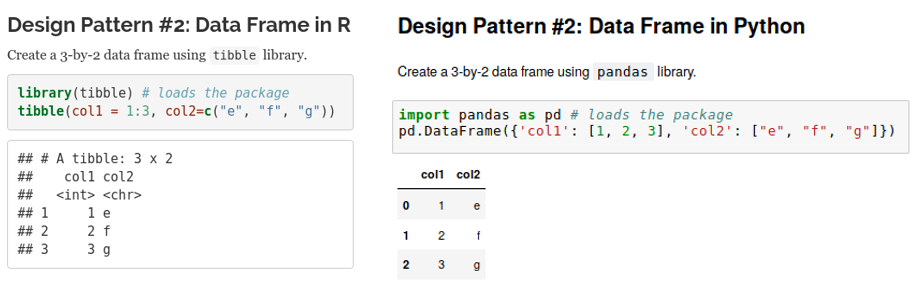
\includegraphics[width=\textwidth+2cm,height=\textheight,keepaspectratio]{images_dp/code_listing_2_df}
\caption[Example for Data Frame Design Pattern.]{The example for \patternName{Data Frame Design Pattern} demonstrates two \emph{data frames} being created. 
While on the left \mintinline{R}/tibble/ is displayed when rendering the previous Figure \ref{lst:code_pattern1}, on the right Python's \mintinline{python}/pandas/ is shown.
The source code for this pattern is located in \path{code_data/R_masterThesis.Rmd} file, \path{code_data/Py_masterThesis.ipynb} respectively.}
\label{lst:code_pattern2}
\end{figure}

%%%%%%%%%%%%%%%%%%%%%%%%%%%%%
\section{Pattern 3: Tidy Data}

\paragraph*{Context}
While \ac{DW} may already store high-quality, rectangular tables in an easy to work with structure, externally captured information is organized in a variety of formats and diverse in their shapes.
After importing it from different \ac{IT} systems and web services, data frames are formatted to facilitate knowledge discovery.
Although processing has been argued to take the largest effort, depending on studies anywhere between 30\% and 80\%, the accurate and clean data stored in a right way make it simple to handle any \ac{DS} task \parencites{ThomasZeutschler2016ITAnalytics}{Taft2015}.

\paragraph*{Problem}
Most typically encountered are messy data which are usually organized in a \emph{wide} format where a table contains one observation (row) across many different variables (columns) for each subject that can be for example a person or a country \parencite{Boehmke2016DataR}. 
Hence, they need to be efficiently changed to become ready for the subsequent analytical investigation. 

\paragraph*{Forces}
\begin{compactitem}
  \item Modifying (big) data by hand may not be accomplished due to their sheer size, complexity and significant time effort leading to potentially introducing errors and having a non-agile \ac{DS} by being distracted from deriving the actionable business results.
  \item At the same time, different \ac{KDD} steps, methods and tools expect one exact arrangement of data forcing professionals to reshape them frequently in the journey through the data pyramid. 
  \item Working with data that may contain several variables \qcite{in one column} or \qcite{in both rows and columns} affects the inquiry on account of having difficulties in their understanding as well as conducting any exploratory operations \parencite[5]{TidyDataWickham2014}.
\end{compactitem}

\paragraph*{Solution}
Spearheaded by \textcite[5]{TidyDataWickham2014}, the concept of \emph{tidy data} has been suggested to \qcite{provide a standard way of structuring a dataset}.
Modelled after \citeauthor{Codd:1970:RMD:362384.362685}'s (\citeyear{Codd:1970:RMD:362384.362685}) third normal form, three core principles were specified, namely (a) each variable forming a column, (b) each observation forming a row and (c) each type of observational unit forming a final table.
As such, this manifests into the \emph{long} data structure where a table spans each subject over multiple observations because of having a column (a key) with variable types such as land area or a population and another one for their corresponding values. 
Being a part of a broader data management where metadata, data stewardship and security are of an importance, the technique of tidying the dataset into a particular layout has become a design convention for organizing analysis-friendly information \parencites{WilsonGred2017}{CMACanada2003}{DataBoK2017}. 

\paragraph*{Consequences} ~\\
{\hspace*{14.5pt} \textbf{Benefits:} \hspace*{-5.5pt} }
Having data in the \emph{long} format simplifies their manipulation and further transformation including filtering or ordering \parencite{NinaBookR2014}.
In this matter, \emph{tidy data} increase users' overall experience by leveraging a consistent approach in coding style due to a potential availability of closely related tools that make the analysis flow easily together, for instance with a sequencing \enquote{\%>\%} pipe operator \parencites{Boehmke2016DataR}{GarrettGrolemund2017RData}.

\textbf{Liability:}
Contrarily, \emph{wide} data might be more straightforward to enter and inspect as they can have column names as values like \enquote{day1} or in ranges such as \enquote{\$10-20k} \parencites{WilsonGred2017}.
Moreover, albeit language neutral, the concept is largely R centric where it stipulates a domain-specific language, a \qcite{sub-dialect of the R} called \emph{tidyverse} -- thus plausibly not directly replicable to other languages \parencite{Rickert2017}. 

\paragraph*{Known Uses}
\begin{compactitem}
  \item Principally, the evidence stored in the \emph{long} style is most frequently imperative for the modelling and visualization purposes and corresponding packages that enable it, see \patternName{Prototyping} and \patternName{Interactive Application Design Pattern} \parencite{TidyDataWickham2014}. 
  \item Within the R's \emph{tidyverse} sub-ecosystem, data in the corresponding shape play an integral role as they work hand in hand with complementary tools, including the previously mentioned \mintinline{r}/tibble/ \parencite{GarrettGrolemund2017RData}.
\end{compactitem}

\paragraph*{Sample code}
For R, a variety of options exist that provide operations for \emph{tidy data}.
When data frames are build using \mintinline{R}/data.table/, it also offers \mintinline{R}/melt()/ and \mintinline{R}/dcast()/ functions for their reshaping which are claimed to outperform the identically titled ones from the original \mintinline{R}/reshape2/ package \parencite{DataTable2017}.
Additionally, within the tidyverse ecosystem, a dedicated application has been developed named \mintinline{R}/tidyr/ too, see its use in Figure \ref{lst:code_pattern4}.

On the contrary, the previously mentioned \mintinline{python}/pandas/ is indispensable in the Python's \ac{DS} ecosystem due to being comprehensive in capabilities it provides, including for data transformation.
Nonetheless, when data are in a more traditional shape of an array or a matrix, \mintinline{python}/NumPy/ library, being a part of the \emph{SciPy} sub-ecosystem, offers its own methods as well.

\begin{figure}[!ht]
\centering
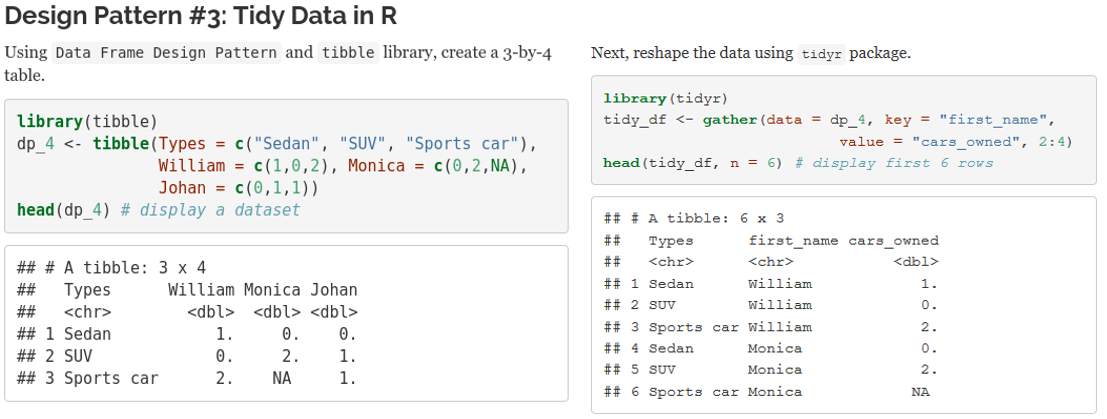
\includegraphics[width=\textwidth+2cm,height=\textheight,keepaspectratio]{images_dp/code_listing_3_td_R}
\caption[Example for Tidy Data Design Pattern.]{An example for \patternName{Tidy Data Design Pattern} shows how a data frame is created using R' \mintinline{R}/tibble/ and subsequently transformed from a \emph{wide} (messy) to a \emph{long} (tidy) format. 
The source code for this pattern is located in \path{code_data/R_masterThesis.Rmd} file, \path{code_data/Py_masterThesis.ipynb} respectively.}
\label{lst:code_pattern4}
\end{figure}

%%%%%%%%%%%%%%%%%%%%%%%%%%%%%%
\section{Pattern 4: Leakage}

\paragraph*{Context}
After data cleaning and formatting, it is still rare that data sets are complete allowing the analysis and modelling to proceed further and make valid conclusions to stakeholders reflecting the stated objectives.
Indeed, when some information is missing or not being in the right quality and quantity, among some not always available and preferred options, it can be crowdsourced from users or be acquired from third-party providers \parencites{Domino2017DS}.

\paragraph*{Problem}
Before \ac{ML} prototypes are created, data scientist need to solve table's missing data as their occurrence is undesirable for many algorithms which often simply omit potentially valuable observations with some lacking values. 
Therefore, the analysis of incomplete facts might be misleading and absent data need to be predicted or otherwise \enquote{imputed}.

\paragraph*{Forces}
\begin{compactitem}
  \item Dropping rows or columns which contain missing values is universally not advisable as it reduces a sample size and introduces a bias to parameter estimates like correlation or standard error \parencite{Gelman2007}. 
  \item At the same time, replacing missingness with median, mode or mean can lead to biased estimates too due to outliers, not considering relationships between features and general uncertainty about the outcomes that is not reflected in the imputed data \parencite{Rubin2002}.
  \item The other so-called \emph{single imputation method} may involve regression where missing values are predicted from complete observations using a regression model. 
  Though, as described by \textcites[6]{ZhangSingleImput2016}{GarcijaGomez2010}, the \qcite{variability of missing values is underestimated} by this approach as only a single regression curve is created. 
\end{compactitem}

\paragraph*{Solution}
In order for data scientists to appropriately handle missing data, one needs to answer an integral question, namely why are they missing.  
According to \textcite[3]{DabneyAlanNormalization2012} three missing data mechanisms are distinguished and consequently the approach to a treatment \qcite{should ideally rely on the mechanism that caused the values to be missing} in the first place. 

\textcite{Rubin2002} have talked about a concept named \emph{missing at random (MAR)} where missing data ($Y_{mis}$) are related to those observed ($Y_{obs}$) and can be predicted from them.
A special case of MAR is when the nature of missing data is not related to input variables -- then data are said to be \emph{missing completely at random (MCAR)}.
This usually happens when the equipment malfunctions or there is an error in data entry -- thus $Y_{mis}$ is neither related to $Y_{obs}$ nor to $Y_{mis}$. 
Both cases are said to be \emph{ignorable} because the reasons for missingness are ignored and \qcite{it is appropriate to impute} such data \parencites[340]{Lynn2002}.
At last, a \emph{nonignorable} situation named \emph{missing not at random (MNAR)} means that the probability of missingness depends on the missing variable itself, for example when a \qcite{sensor cannot acquire [statistics] outside a certain range} \parencites[266]{GarcijaGomez2010}{Grahama2002}{Gelman2007}.

Even though, the best solution is not to have missing data, an advanced statistical model can be specified to predict missing values \parencite{Hasan2017}. 
Particularly under the MAR condition, of a great interest to data scientists should be \emph{multiple imputation} where missing values are imputed $m$ (typically three to twenty) times creating $m$ complete but different datasets \parencite{Grahama2002}.
Then, a study of such missing data is conducted and finally results are pooled (averaged) together by incorporating the \qcite{variability between [and within] the $m$ analyses} \parencite[340-341]{Lynn2002}.

\paragraph*{Consequences} ~\\
{\hspace*{14.5pt} \textbf{Benefits:} \hspace*{-5.5pt} }
If the underlying assumptions were met, \emph{multiple imputation} allows missing data to be accounted for in a statistically valid and unbiased way \parencite{Hasan2017}.
Showing to be flexible and performing well under the different conditions, it reflects the uncertainty of true missing values due to having multiple sets of complete data which are combined to derive final results -- by preserving the sample size and using all available information \parencites{Lynn2002}{Grahama2002}.

\textbf{Liability:}
When data set is large and contains significant amount of missingness, \emph{multiple imputation} becomes complex to compute (due to creating a \enquote{right} model), analyse and combine together \parencite{HortonNickKen2007}.  
Even though selecting a single best-looking imputation can be necessary for the \patternName{Prototyping} task, it is important to keep in mind that true values do not exists, and thus these proxies cannot be taken with absolute certainty \parencite{MittagNik2013}. 

\paragraph*{Known Uses}
\begin{compactitem}
  \item The complete case analysis can be considered when only a very small amount of data is missing ($\leq 5\%$) and being under the MCAR condition \parencites{Grahama2002}{AzurMellissa2011}{imput2006}. 
  \item The simplistic methods of mean and regression treat an imputed single value as a true point. 
  Yet, both make biased estimates too as they fail to account for variability in the data and should not be generally used \parencites{Takahasi2012}{BaraldiCraig2010}.
  \item \textcites{Grahama2002}{AzurMellissa2011} have recommended two state-of-the-art approaches which are aforementioned \emph{multiple imputation} and its a basic alternative called \emph{maximum likelihood with expectation-maximization (EM) algorithm} further described by \textcites{BaraldiCraig2010}{GarcijaGomez2010}.
\end{compactitem}

\paragraph*{Sample code}
Given R's strong statistical foundations, a variety of packages exist that address imputation of missing data. 
Notable of these are \mintinline{R}/mice/ and \mintinline{R}/VIM/. 
On the other hand, for Python and exploration of missing data, data scientists can utilize \mintinline{python}/missingno/ package while for the actual imputation \mintinline{python}/fancyimpute/ library shown in Figure \ref{lst:code_pattern4Leak}.

\begin{figure}[!ht]
\centering
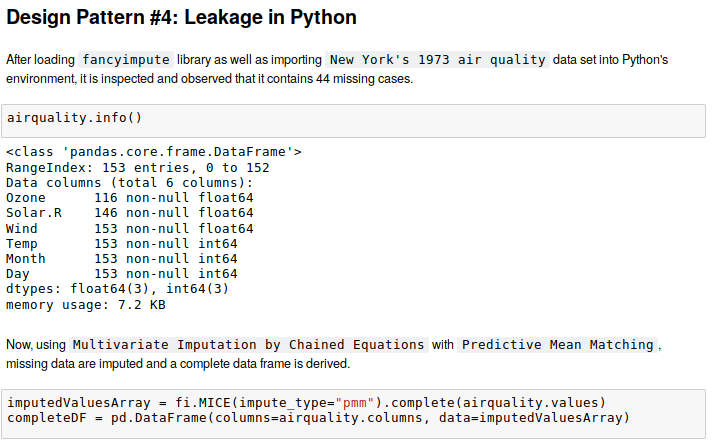
\includegraphics[width=\textwidth+2cm,height=\textheight,keepaspectratio]{images_dp/code_listing_4_leakage}
\caption[Example for Leakage Design Pattern.]{An example for \patternName{Leakage Design Pattern} shows how missing data can be imputed using Python's \mintinline{python}/fancyimpute/ package.
The source code for this pattern is located in \path{code_data/Py_masterThesis.ipynb} file, \path{code_data/R_masterThesis.Rmd} respectively.}
\label{lst:code_pattern4Leak}
\end{figure}

%%%%%%%%%%%%%%%%%%%
\section{Pattern 5: Prototyping}
\paragraph*{Context}
Executives have described in accordance with specific, measurable, assignable, realistic and time-related (SMART) criteria multiple deliverables that they want to receive with a goal of addressing their clients in a better way, and therefore increasing their value to the company.
Such mapping of a business problem to \ac{DS} tasks might include data acquisition and mainly classifying clients into different segments, based on the past transactions predicting sales for the next month and developing simple association rules which might recommend them purchasing new products.

\paragraph*{Problem}
After understanding the nature of data through the exploratory analysis, their transformation, cleaning and potentially imputing missing values, clients need to be classified, sales be predicted and recommendations have to be provided.
Therefore, data scientists need to experiment with simple and complex algorithms that permit them to gain useful insights.

\paragraph*{Forces}
\begin{compactitem}
  \item Having a decisive impact on answering business relevant questions, a variety of statistical models and families exist from which professionals have to identify the right ones and evaluate their performance in line with stated intentions as they all differ in the purpose, interpretability, complexity and accuracy \parencite{SAS2016}.
  \item Furthermore, numerous \ac{ML} applications have become influential as they are flexible for diverse sets of data, easily extensible accommodating new models and metrics and permitting to store intermediate modelling results as well -- all leading to lowering the \ac{DS} bar \parencites{GoebelMichGru1999}{ChenMinMao2014}{EslamiAli2012}.
\end{compactitem}

\paragraph*{Solution}
\ac{KDD} professionals have to identify comprehensive and modular \acp{API} that offer appropriate algorithms for developing \ac{ML} \emph{prototypes}. 
Subsequently, these shall be evaluated to understand how the predictive models perform on unseen data in the future.

When collected information is labelled through attributes, (semi-)supervised learning methods such as \acp{SVM} or naive Bayes are used for predicting the output from input data. 
Depending on different learners and the analytical problem dealt with, two groups of supervised tasks are distinguished -- a \emph{classification} where a target variable is a discrete category or a \emph{regression} where a prediction is a continues numerical value.
On the other hand, when data are unlabelled with no response variable $Y$, more exploratory, unsupervised learning algorithms like $k$-means clustering or principal component analysis are employed to establish groups of similar objects or reduce dimensionality of data \parencites{SAS2016}{NinaBookR2014}.

Continuing with supervised learning, using a \emph{holdout} approach, entire data are at first divided into training (typically about 75\%) and testing set (remaining 25\%; \cite{Kohavi:1995:SCB:1643031.1643047}).
Then, chosen algorithms together with training data are applied for model building. 
Because evaluating prototype's performance on the same data does not tell how well it generalizes, a model is taken with a holdout set to predict outputs and compare its forecast's capability with true data \parencites{FosterProvost2013DataThinking}{JakeVanderPlas2016PythonHandbook}.

\paragraph*{Consequences} ~\\
{\hspace*{14.5pt} \textbf{Benefits:} \hspace*{-5pt} }
\ac{ML} is applicable to diverse industries and use cases and when appropriately applied, a wisdom can be gained which helps decision makers to set right company's objectives and improve products and services to better serve their customers.
Additionally, reflecting the goals, a variety of prototyping metrics can be used for assessing final prediction. 
For example, for classification a confusion matrix is used which \qcite{summarizes the (\dots) predictions against the actual known} classes \parencite[94]{NinaBookR2014}.

\textbf{Liability:}
When complex models are applied, there is a danger of running into a lack of their interpretability \parencite{NadaML2004}. 
Hence, they need to be justified in addition to being regularly updated, verified and improved reflecting changing business operations \parencite{SAS2016}.
Building models may at times also lead to dead paths and accordingly it is necessary to learn quickly from mistakes, and thus maintaining a hub of the past work can support the organization in gaining the knowledge \parencites{Domino2017DS}{SASBP2007}{GoogleDebt1}.
Insufficient quality and quantity of data has a significant impact on the model's predictive power too and for that reason data scientists have to constantly iterate on created prototypes and gather better information \parencites{Zinkevitch2016}{CarlShan2015TheScientists}.

\paragraph*{Known Uses}
\begin{compactitem}
  \item In the unsupervised learning, typical tasks include segmenting (clustering) movies according to the user preferences or creating association rules where market basket analysis establishes customers' items that are frequently bought together \parencites{Trevor2017}{ClusteringAnil2010}{Movies2012}{MBAMR2012}. 
  Furthermore, when data have many potentially redundant features, one may benefit from quicker computation by attempting to reduce $d$-dimensions into $m$ principal components that explain most of the variance in the data \parencites{FieldCadyDSBook}{Tillburg2009}.
  \item In the supervised learning, in the case of regression, it has been attempted for example to predict forest's burned area based on the meteorological data \parencite{ForestFires2007}.
  On the other hand, detecting spam emails has been extensively studied by many researchers as a conventional classification problem \parencite{Brylspam2008}.
\end{compactitem}

\paragraph*{Related patterns}
The exposure to the \emph{bias-variance trade-off} has to be addressed as it can make \ac{ML} prototypes not generalizable beyond the training data, see next \patternName{Cross-validation Design Pattern}.
In addition, \ac{ML} libraries and frameworks have support a range of other capabilities such as later described hyperparameter optimization using \patternName{Grid} or leveraging ensemble methods through \patternName{Assemblage Design Pattern}.

\paragraph*{Sample code}
Because of being in the context of a specific task, an illustrative \mintinline{bash}/Pima Indians Diabetes/ dataset is obtained from \textcite{Lichman:2013} to predict whether females of Pima Indian heritage have diabetes, being a binary classification task. 
Consequently, this is used for illustration in the following three patterns as well. 

In the R ecosystem, two prominent packages exist that provide comprehensive tools for building and evaluating models -- \mintinline{R}/caret/ and \mintinline{R}/mlr/. 
For Python, multiple alternatives are available too, most notably well-established \mintinline{python}/scikit-learn/ for general-purpose \ac{ML}. 

\begin{figure}[!ht]
\centering
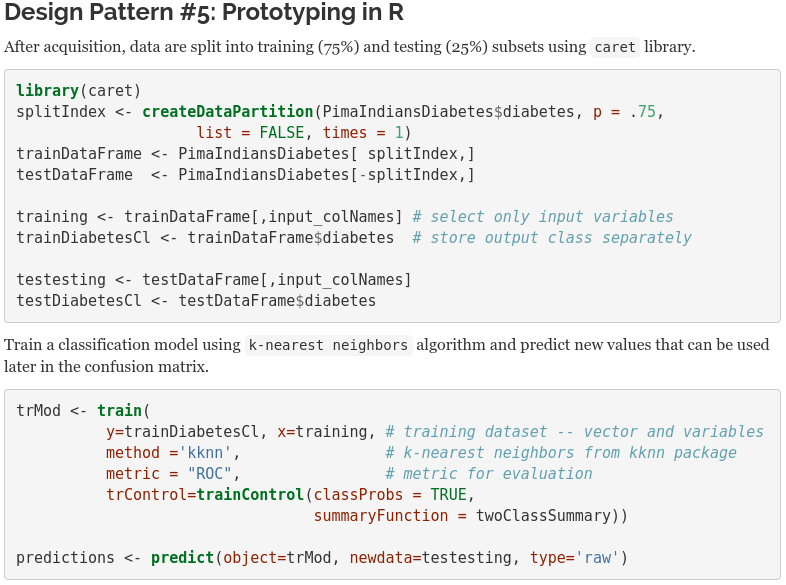
\includegraphics[width=\textwidth+2cm,height=\textheight,keepaspectratio]{images_dp/code_listing_5_prototype}
\caption[Example for Prototyping Design Pattern.]{An example for \patternName{Prototyping Design Pattern} shows R's \mintinline{R}/caret/ library when applied for a classification task using a holdout approach.
The source code for this pattern is located in \path{code_data/R_masterThesis.Rmd} file, \path{code_data/Py_masterThesis.ipynb} respectively.}
\label{lst:code_pattern5}
\end{figure}
%%%%%%%%%%%%%%%%%%%%%%%%%%%%
\section{Pattern 6: Cross-validation}

\paragraph*{Context}
After initial understanding of preferably \emph{tidy} data and the domain being dealt with, a supervised learning algorithm was selected to plausibly satisfy stakeholders' objectives.
Succeeding the \patternName{Prototyping Design Pattern}, the model has to be evaluated as it may not generalize beyond the data which have been used for its creation, causing \emph{overfitting}. 
This means that while originally the learner scored highly on the training data, when previously unseen information arrives, prototype's high complexity leads to a very poor accuracy of a new prediction as it fits noisy data \parencite{NinaBookR2014}.

\paragraph*{Problem}
A major task for any data scientist is to balance the so-called \emph{bias-variance trade-off} where on the one hand \ac{ML} prototype has to account for relevant data features (have high accuracy; in statistical terms low bias) while on the other hand also avoid capturing meaningless data -- that is to have high precision, statistically low variance \parencite{JakeVanderPlas2016PythonHandbook}.
Consequently, one needs to assess learner's predictive power with future data samples using a robust technique which could aid in selecting a model with the lowest bias and lowest variance \parencite{Kohavi:1995:SCB:1643031.1643047}.

\paragraph*{Forces}
\begin{compactitem}
  \item If training and testing prototypes on the same data set, they \enquote{memorize} them very well but this is not representative of the general data trend \parencites{FosterProvost2013DataThinking}{SAS2016}.
  \item Previously, a classical approach tackling overfitting was described where data are randomly split into two sets. 
  This makes a fair approximation by holding back some of the data to validate the prototype with new information.
  However, a portion of valuable data is not training the learner as the test set may be significantly influenced when a random split is not characteristic and balanced \parencites{NinaBookR2014}{FosterProvost2013DataThinking}. 
  \item Although a frequently named alternative is partitioning data into three sets (training, validation and testing), because they are usually small in sample size, a number of examples for \ac{ML} is further reduced. 
  Hence, either holdout approach excludes some information and prevents learning from complete data patterns \parencite{FieldCadyDSBook}.
\end{compactitem}

\paragraph*{Solution}
\emph{Cross-validation} is a sophisticated method for \qcite{generat[ing] multiple performance measures} with an ability to tell what to expect from the forthcoming data by estimating test set (so-called generalization) error \parencite[140]{FosterProvost2013DataThinking}. 
Enhancing the basic holdout technique, it repeats \qcite{the construction of the model on different subsets of the available training data and then evaluate[s it] only on data not seen during construction} \parencite[111]{NinaBookR2014}.

The widely used \emph{k-fold cross validation} splits a data set into $k$, typically five or ten, folds with a goal of training and scoring the prototype $k$ times \parencite{FosterProvost2013DataThinking}.
In each iteration of the cross-validation, $k-1$ different partitions are combined on which the learner is trained and finally its accuracy is estimated on the last fold deriving the overall test performance. 
Having multiple results, these are united by mean for checking the bias and standard deviation for the variance \parencite{NinaBookR2014}.

\paragraph*{Consequences} ~\\
{\hspace*{14.5pt} \textbf{Benefits:} \hspace*{-5pt} }
Compared to the holdout technique described in the \patternName{Prototyping Design Pattern} or \emph{bootstrapping} outlined next, each sample created from cross-validation is certainly used for training and testing step, resulting into reducing the bias as the number of $k$ parts increases \parencite{Gutierrez-Osuna2002LECTURECross-validation}.
Even though it has been sometimes argued that when cross-validation is repeated multiple times, model's variance decreases too, some researchers have not been able to confirm this hypothesis \parencites{Vanwinckelen2012OnCross-validation}{Kohavi:1995:SCB:1643031.1643047}. 

\textbf{Liability:}
Cross-validation is computationally (very) expensive as training and testing steps are rerun $k$ times, specifically with a variation called \emph{leave-one-out cross validation}. 
Despite $k=n$ number of examples, results can still exhibit high variance as well \parencite{Gutierrez-Osuna2002LECTURECross-validation}.

\paragraph*{Known Uses}
\begin{compactitem}
  \item When new data cannot be acquired, cross-validation often becomes \emph{the} method for model building and selection in \ac{DS} through its universality and simplicity \parencites{arlot2010}{CVStandart2008}.
  \item Besides \emph{k-fold cross validation}, variations such as \emph{stratified} or \emph{repeatable cross-validation} have been proposed as well.
  Whereas the objective of the former one is to address biased classes, thus balancing the distribution across each fold making it a good representative of the whole sample, the goal of the latter one is to repeat cross-validation $n$ times creating random data folds whereby subsequent predictions can all be averaged \parencites{KuhnMax2013}{Vanwinckelen2012OnCross-validation}. 
\end{compactitem}

\paragraph*{Related patterns}
As seen next, \emph{cross-validation} is frequently used with the \patternName{Grid} and \patternName{Assemblage Design Pattern}, particularly with the latter one which has the capability of further reducing the overfitting \parencite{NinaBookR2014}. 

An alternative method to cross-validation represents \emph{bootstrapping} which is mainly used for obtaining confidence intervals and where a random sample with replacement of the same size as the original data set is taken for the training step. 
Then, the model is trained on each of them and before results are again averaged, it is also tested on the remaining \qcite{examples that were not selected for training} \parencites{Kohavi:1995:SCB:1643031.1643047}{BookCV201}{Gutierrez-Osuna2002LECTURECross-validation}.  

\paragraph*{Sample code}
Using previously identified R's \mintinline{r}/caret/ and Python's \mintinline{python}/scikit-learn/, a naive Bayes model is demonstrated next where it is applied to four data parts and tested on the fifth one, see Figure \ref{lst:code_pattern7}. 

\begin{figure}[h]
\centering
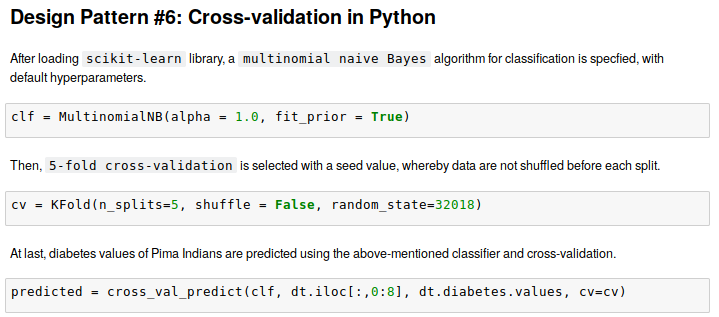
\includegraphics[width=\textwidth,height=\textheight,keepaspectratio]{images_dp/code_listing_6_cv}
\caption[Example for Cross-validation Design Pattern.]{The example for \patternName{Cross-validation Design Pattern} shows application of \mintinline{python}/scikit-learn/ whereby data are first split using five-fold cross validation to which a \emph{multinomial naive Bayes} classifier is applied. 
The complete source code for this pattern is located in \path{code_data/Py_masterThesis.ipynb}, \path{code_data/R_masterThesis.Rmd} respectively.}
\label{lst:code_pattern7}
\end{figure}

%%%%%%%%%%%%%%%%%%%%%%%%%%%%%%
\section{Pattern 7: Grid}

\paragraph*{Context}
\emph{Hyperparameters} are specified in the model before a training step can begin.
While some algorithms have none and can be immediately used for a particular task, others like $k$-means clustering or random forest contain several that data scientists are required to set. 
Typically, in the latter case, one has to decide on a number of trees to build before averaging their predictions \parencite{DL2016Mit}. 
Overall, the importance of hyperparameters lies in having a significant influence on various costs of running the prototype as well as on its behaviour and final performance as seen for instance from \patternName{Prototyping Design Pattern}.

\paragraph*{Problem}
Instead of making (non-)educated guesses to find best hyperparameters by trial-and-error, it is desirable to have an automatic procedure that optimizes them and therefore can increase model's predictive power, its robustness and ultimately generalizability when facing new data.

\paragraph*{Forces}
\begin{compactitem}
  \item Albeit most frequently applied, searching manually for hyperparameters is very time-consuming effort because of their number and having necessary understanding of what they do and what impact they have on the learner \parencite{DL2016Mit}. 
  \item Moreover, retraining each time the prototype because of manually adjusting a large set of hyperparameters can probably lead to omitting some better values.
\end{compactitem}

\paragraph*{Solution}
While designing \ac{DS} pipeline, professionals should employ \emph{grid search} which identifies hyperparameters that deliver best predictions. 
At first, a finite set of values for each hyperparameter is specified in a \emph{grid} which can be in a matrix form through employing \patternName{Data Frame Design Pattern}, simplified for instance \mintinline{bash}/{'k':[2, 4, 6/, \dots, $j$\mintinline{bash}/]}/ and \mintinline{bash}/{'size':[10, 100, 1000/, \dots, $i$\mintinline{bash}/]}/.
Subsequently, the \emph{grid search} algorithm takes the Cartesian product of previous sets $(i_{1...n} \times j_{1...n})$ with $n \in \mathbb{N}_{>0}$ and uses all combinations for training the model \parencite{JakeVanderPlas2016PythonHandbook}. 
After evaluating its performance, typically, by means of \patternName{Cross-validation Design Pattern}, the outcome of such comprehensive search allows to find best settings that should be utilized \parencite{DL2016Mit}.

\paragraph*{Consequences} ~\\
{\hspace*{14.5pt} \textbf{Benefits:} \hspace*{-5pt} }
Even though not guaranteed, choosing a right set of hyperparameters can boost learner's predictive strength by easily parallelizing the computation across a cluster of machines \parencite{BreckMLTest2016}.
Due to being a fairly general approach, one can optimize not only hyperparameters themselves but also finding out the most excellently performing \ac{ML} prototype as well.

\textbf{Liability:}
Searching for best hyperparameters is very \ac{CPU} intensive operation that increases modelling expenses exponentially, particularly when their number to fix is large.
Besides being of $\mathcal{O}(n^c)$ time complexity with $c$ hyperparameters and $n$ number of their values, determining the optimal \emph{grid} to search in may be a task for itself, thus the reliance on experience and third-party resources where similar data or methods were applied \parencite{DL2016Mit}. 

\paragraph*{Known Uses}
Hyperparameter optimization may still lead to overfitting and therefore one ought to combine it with \patternName{Cross-validation Design Pattern} \parencites{JakeVanderPlas2016PythonHandbook}{minleegrid2005}. 
In order to ensure forecast's high-quality, data are at first divided into the training and testing part.
Then, cross-validation splits the training set into $k$-folds. 
For each Cartesian product from the \emph{grid}, a model is trained $k-1$ times and tested on the subset that was left out, leading to record the highest average performance for a particular instance with specific settings.
At last, the one with the best results would be selected for the final step of testing the data from their first separation \parencite{Olson2008}.

\paragraph*{Related Pattern}
Besides aforementioned \emph{grid} and \emph{manual search}, scientists such as \textcites{ReviewHyperOpt2015}{SAS2016} have described other techniques of tuning hyperparameters that have shown to be more convenient and efficient too. 
One of the alternatives presented by \textcite{Bergstra2012RandomOptimization} is named \emph{random search} which takes an arbitrary sample of specified parameters from the \emph{grid} space using a probability distribution like Bernoulli. 
This has proved to achieve very similar results compared to the exhaustive \emph{grid search} but much faster.

\paragraph*{Sample code}
Generally, the majority of comprehensive \ac{ML} packages like those from \patternName{Prototyping Design Pattern} already offer functionality for hyperparameter optimization, including \emph{grid} and \emph{random search}.
Previously used applications \mintinline{r}/caret/ and \mintinline{python}/scikit-learn/ are examples of it.
Consequently, in Figure \ref{lst:code_pattern8}, \mintinline{r}/caret/ package trains a naive Bayes model five times and evaluates it by applying a \patternName{Cross-validation Design Pattern}.

\begin{figure}[h]
\centering
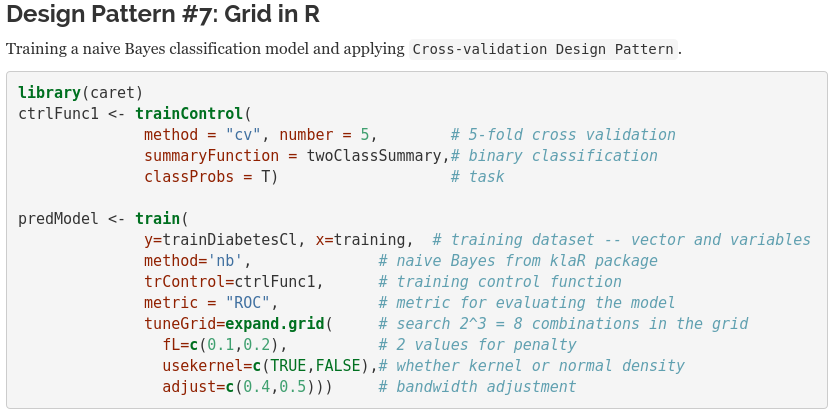
\includegraphics[width=\textwidth,height=\textheight,keepaspectratio]{images_dp/code_listing_7_grid}
\caption[Example for Grid Design Pattern.]{The example for \patternName{Grid Design Pattern} show how naive Bayes model can be trained with \mintinline{r}/caret/ library. 
More specifically, searching the grid with eight hyperparameters and applying five-fold cross-validation.
The complete source code for this pattern is located in \path{code_data/R_masterThesis.Rmd}, \path{code_data/Py_masterThesis.ipynb} respectively.}
\label{lst:code_pattern8}
\end{figure}

%%%%%%%%%%%%%%%%%%%%%%%%%%%%%%
\section{Pattern 8: Assemblage}

\paragraph*{Context}
In the \patternName{Prototyping Design Pattern} it was noted that multiple different algorithms could be used for unsupervised and supervised learning. 
Particularly in the latter case, after training a baseline model and even optimizing its hyperparameters, data scientists ought to judge its performance not only by distinct metrics but also see it in the context of other prototypes to better understand how they behave and compare to each other.
All that in line with \ac{DS} premise of being an iterative process where several alternatives should be build and evaluated.

\paragraph*{Problem}
To further improve achieved results, besides increasing volume of data and their quality through extensive pre-processing, applying for instance \patternName{Leakage Design Pattern} and engineering new features, data scientists may need to intelligently combine outcomes of many diverse models for gaining a greater predictive accuracy in contrast to individual methods alone. 

\paragraph*{Forces}
\begin{compactitem}
  \item A multitude of tested estimators display only mediocre conclusions that are just slightly above a random guess. 
  \item Moreover, even though cross-validation and grid search were administered, it is still possible to observe overfitting that hinders model's practical use for business purposes.
  \item The developed \ac{ML} prototypes carry a large variance due to randomness in hyperparameters, probabilistic nature and selection of data \parencite{NinaBookR2014}.
\end{compactitem}

\paragraph*{Solution}
In the quest of designing high-quality model which is capable of \qcite{reduc[ing] the effect of (\dots) overfitting}, engineers may leverage the power of so-called \emph{ensemble methods} \parencite[426]{JakeVanderPlas2016PythonHandbook}.
These integrate a collection of modelling instances from families such \ac{SVM} or naive Bayes that are diverse and likewise perform differently on the same data \parencite{NagiSajid2013}.
Consequently, their \emph{assemblage} shall lead to improved outcomes and especially \emph{stacking} has been a prominent method. 
This leverages an independent and simple meta-model that combines other prototypes where at first they are individually trained in order to acquire not only their original features but predicted outputs too. 
Then, in the final step of meta learning, the base-level classifiers are basically \enquote{blended} by the super learner algorithm to possibly derive better results \parencites{EnsembleML2012}{Opitz1999}.

\paragraph*{Consequences} ~\\
{\hspace*{14.5pt} \textbf{Benefits:} \hspace*{-5.5pt} }
\emph{Assemblage} of methods attempts to address an instrumental trade-off in \ac{DS}, namely reducing both high variance while at the same time high bias as well \parencite{JakeVanderPlas2016PythonHandbook}. 
Indeed, the accumulation of prototypes has shown to potentially improve final accuracy of prediction by lowering generalization error on unseen data, notably when they contain high amount of variables along with being small in the sample size \parencites{NinaBookR2014}{EnsambleBioinf2010}.

\textbf{Liability:}
Being frequently applied with the \patternName{Grid} and \patternName{Cross-validation Design Pattern}, all three add to the required computing resources \parencite{EnsembleML2012}. 
Primarily, however, \emph{assemblage} further hampers conclusion's interpretability and understandability by the managers creating an undesirable black-box \parencite{PeterETHZ2012}.
Furthermore, if predictions are strongly correlated, one will not be able to boost them with the \emph{ensemble} \parencite{FosterProvost2013DataThinking}. 

\paragraph*{Known Uses}
\begin{compactitem}
  \item Due to universally claiming to improve returns on data of various quality and quantity, practical applications include winning \ac{DS} competitions like Netflix Prize in 2009 where \emph{Gradient Boosted Decision Trees} were applied on hundreds of individual learners to improve company's recommendation engine, see \textcite{Netflix2009}.
  \item \textcites{GranaMichal2014}{NagiSajid2013} have described other use cases such as improved detection of cyber-attacks, prevention of financial fraud, avoiding credit risk or in the medicine for diagnosis of diseases.
\end{compactitem}

\paragraph*{Related Pattern}
Although \emph{stacking} is one of the more advanced \emph{assemblage} techniques, other approaches exist as well \parencite{SAS2016}. 

Considering random forests, these aggregate results from decision trees that are build using training subsets of data sampled with replacement and only with random features \parencite{NinaBookR2014}.
By decreasing the variance, trees can be averaged in parallel to derive the best estimator -- the procedure of which is called \emph{bagging} \parencites{Opitz1999}{PeterETHZ2012}. 

In contrast, \emph{boosting} algorithms like AdaBoost reduce the bias and variance by incrementally building in sequence several \enquote{weak} models that are often only barely better than a random guess \parencite{EnsambleBioinf2010}. 
Aiming to build a combined \enquote{strong} classifier, the idea is to learn from misclassifications of a model instance which culminates into reweighting training data at each round to emphasize shortcomings that should be addressed with a new iteration \parencite{EnsembleML2012}.
Though, not being a silver bullet, overfitting can still occur with outliers and other noise in the data \parencite{BauerErikChan1999}.

\paragraph*{Sample code}
For R, one can use an extension to the previously mentioned \mintinline{R}/caret/ library called \mintinline{R}/caretEnsemble/ or among others \mintinline{R}/SuperLearner/ package. 
Contrarily, besides already shown Python's \mintinline{python}/scikit-learn/ that can be supplemented with \mintinline{python}/Mlxtend/, the example in Figure \ref{lst:code_pattern9} creates an ensemble of two methods using \mintinline{python}/ml-ensemble/ utility. 

\begin{figure}[h]
\centering
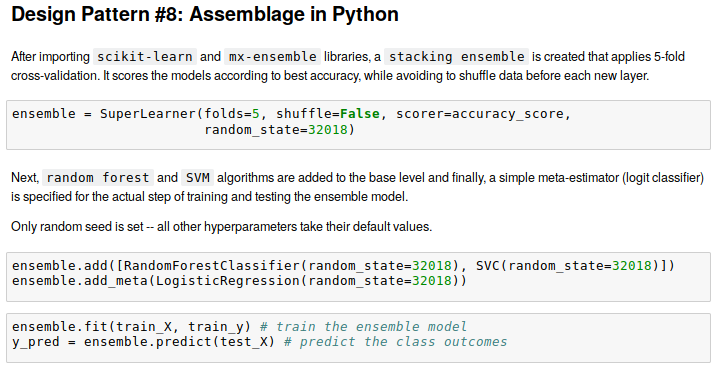
\includegraphics[width=\textwidth,height=\textheight,keepaspectratio]{images_dp/code_listing_8_ensam}
\caption[Example for Assemblage Design Pattern.]{The example for \patternName{Assemblage Design Pattern} displays how a \emph{stacking (logit classifier) ensemble} is constructed to use features from training data through \ac{SVM} and random forest in its resulting prediction.
The complete source code for this pattern is located in \path{code_data/Py_masterThesis.ipynb}, \path{code_data/R_masterThesis.Rmd} respectively.}
\label{lst:code_pattern9}
\end{figure}

%%%%%%%%%%%%%%%%%%%%%%%%%%%%%%
\section{Pattern 9: Interactive Application}

\paragraph*{Context}
After acquiring information about business activities and having answers to questions asked, being one of the concluding steps is when findings are visually communicated in an effective and understandable manner to stakeholders. 
This is done in order to add value to offered services and products and deliver return on \ac{DS} investment.

\paragraph*{Problem}
While the diversity of employee's background and roles manifests in seeking different perspectives to the same underlying data, this is not aligned with conventional reports and presentations which usually display static visualizations and are limited by their scope and a particular view presented -- hence the need for a better alternative.

\paragraph*{Forces}
\begin{compactitem}
  \item Referencing big data properties, information changes rapidly and therefore static graphics may not be relevant in one-week time and so the conclusions based on them. 
  \item Storytelling requires to visualize not only latest data but also enable audience to answer their questions by themselves through adjusting the way information is conveyed in an interactive fashion, for example by drilling it down, without unnecessary latency \parencite{TabPatriVisual2015}.
  \item Business managers are usually not interested in pure numbers without a context and explanation, and thus interpretable results told through diverse means that can easily translate into a set of operational processes and actions are indispensable \parencite{FosterProvost2013DataThinking}.
\end{compactitem} 

\paragraph*{Solution}
As an important part of the communication strategy, data scientists shall design and develop simple, web-based \emph{interactive applications} using the identical programming language applied for other \ac{DS} tasks to stay within the same workflow and avoid technological fragmentation.
Indeed, such applications have to permit users to dynamically interact with presented tables or charts and customize them for their data journey by modifying various graphical and data attributes that reflect employees' own preferences, for instance filtering, zooming or changing the shapes \parencite{WardInteractiveApps2010}. 

\paragraph*{Consequences} ~\\
{\hspace*{14.5pt} \textbf{Benefits:} \hspace*{-5.5pt} }
Stakeholders are provided with a self-service tool that empowers further data exploration, gaining deeper insights by looking at information tooltips and understanding the story through animations and slideshows. 
The information being updated in close to real time makes visualizations display latest available data and consequently fostering a trust and a deeper integration in the organization by allowing to proactively react to the changing environment \parencites{Domino2017DS}{FieldCadyDSBook}.

\textbf{Liability:}
Developing high-quality \emph{interactive application} carries an additional effort in its continuous maintenance due to ever evolving data sources, their granularity and employee desires \parencites{Clarke2013}{Fern2016}. 
Furthermore, it is necessary to understand the targeted technology platform and learn tools for its development.
Besides, when the application has been improperly designed displaying excessive details, technical jargon or having a misguides choice of colours, it ultimately contributes to information overload and never being looked at \parencites{InformaVisualiz}{Gershon1998}{Carr1999}{TabPatriVisual2015}. 

\paragraph*{Known Uses}
\begin{compactitem}
  \item \textcites{DickInteractive2014}{SegelHeer2010} have indicated that interactive stories may possibly enhance a reading experience of a journalistic work on the web.
  \item As already mentioned in the \patternName{Notebook Design Pattern}, dynamic visualizations can be embedded in the document making data analysis more visual from the beginning.
  \item \ac{BI} portals, following best practises in the \ac{UI/UX} design, make available a standard set of core components like sliders for creating \ac{KPI} dashboards with interactive plots.
\end{compactitem}

\paragraph*{Related patterns}
Besides having \emph{interactive applications} on-premise, organizations can take advantage of \emph{cloud computing} services run by providers like Microsoft (\emph{Azure}) or Amazon (\emph{Web Services}). 
This in order to leverage features such as automatic scaling that ensures their uninterrupted availability, see next \patternName{Cloud Design Pattern}. 

\paragraph*{Sample code}
While \mintinline{R}/Shiny/ is almost certainly the most widely used package for developing analytical and interactive web application using R, for Python besides \mintinline{python}/Bokeh/ one can create them by utilizing \mintinline{python}/Plot.ly Dash/ framework too, see Figure \ref{lst:code_pattern10}.

\begin{figure}[ht]
\centering
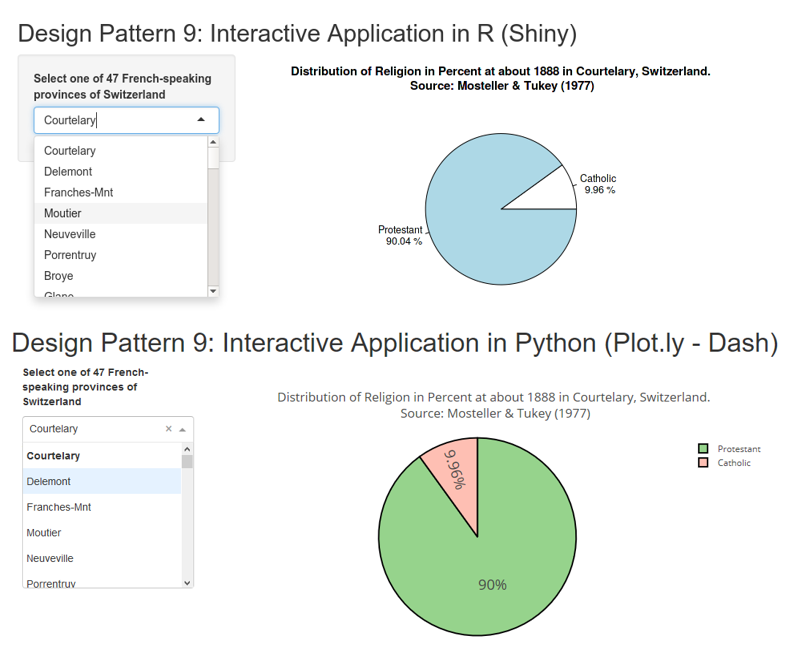
\includegraphics[width=\textwidth,height=\textheight,keepaspectratio]{images_dp/code_listing_9_intApp}
\caption[Example for Interactive Application Design Pattern.]{The example for \patternName{Interactive Application Design Pattern} shows exceptionally a result of R and Python source code located in \path{code_data/dp_9} folder. 
A simple pie chart with a dropdown component where users can choose from a list of provinces is displayed. 
This shows a distribution of religion in Switzerland based on the \emph{Swiss Fertility and Socioeconomic Indicators (1888)} data, obtained through R's \mintinline{R}/datasets/ library.
Upon changing the region (the user interaction), the chart is immediately redrawn to reflect new values.}
\label{lst:code_pattern10}
\end{figure}

%%%%%%%%%%%%%%%%%%%%%%%%%%%%%%
\section{Pattern 10: Cloud}

\paragraph*{Context}
After making available on a local machine a proof of concept which is subsequently validated first by peers in the \ac{DS} team and later by directly involved customers themselves, it is necessary to share the solution with all stakeholders of the organization by deploying it on the production system.

\paragraph*{Problem}
Data scientists need to utilize computing resources in a flexible and simple matter without being constrained by the available hardware and software at company's premises.
The objective of this is to allow for instance quickly scaling up and down \ac{DS} interactive applications or integrating complex predictive models into firm's products and services.

\paragraph*{Forces}
\begin{compactitem}
  \item Organization's core mission is often unrelated to administrating and configuring hardware and software infrastructure. 
  To avoid facing various constrains and difficulties, it has been claimed of being beneficial to outsource the management of servers to experienced specialists \parencite{MarstonSean2011}.
  \item Training \ac{ML} models as well as pre-processing (big) data requires significant computing resources which might impede fast prototyping of \ac{DS} solutions because of the unavailability of modern, on-premise \acp{CPU}, high-volume storage systems and \ac{RAM} in the necessary quantity. 
\end{compactitem}

\paragraph*{Solution}
Instead of building and maintaining own infrastructure, companies and data scientists should learn to utilize \emph{cloud computing} made available by vendors like Google (\emph{Cloud}) or Microsoft (\emph{Azure}). 
While many different types of \emph{cloud} services exist, see \textcite{Zhang2010CloudChallenges} for their overview, a core underlying feature is the ability of on-demand allocation of computing resources paid according to the pay-as-you-go pricing model.  
As such, the \ac{IT} architecture including \ac{DS} workflow shall be designed around leveraging \emph{cloud} features where dedicated data mining virtual machines or enhanced applications for information storage and processing based on the \emph{Hadoop} toolbox might be employed.

\paragraph*{Consequences} ~\\
{\hspace*{14.5pt} \textbf{Benefits:} \hspace*{-5.5pt} }
Perhaps the most important gain is avoiding managing on-premise infrastructure where instead a \emph{cloud} portal permits a rapid provisioning of resources as they are deemed necessary by engineers.
Additionally, it allows to scale organization's \ac{IT} architecture organically and due to using a comprehensive platform which integrates with other offered functionalities, data scientists can focus on understanding the data by taking advantage of a full set of related services \parencites{DJ2013}{Fern2016}.

\textbf{Liability}:
Besides potentially expensive and hence necessity of monitoring used resources, selecting one provider can result into a vendor lock-in because of unique features that may not exist at competitors (or work in a similar matter; \cite{JusticeMartinis2015Cloud}). 
Moreover, security and privacy concerns can put \emph{cloud computing} either in jeopardy or substantially increase technological and bureaucratic burdens due to legal compliance and regulations \parencite{StoneAdamPrivSecCloud2010}.
Furthermore, companies may not be culturally and process-wise ready to take its advantages by reasons of lacking in-house expertise.

\paragraph*{Known Uses}
\begin{compactitem}
  \item Typically, the power of \emph{cloud} complements natural language processing or object recognition in images and at the same time enables quicker training of predictive models and management of the whole \ac{DS} workflow and \ac{ETL} pipeline.
  \item Likewise, third-party \emph{cloud} services can reinforce good software engineering practises such as continuous integration and platform agnostic development and deployment \parencite{GuhaSEngCloud2010}. 
  \item \ac{KDD} newcomers without programming skills may use various \emph{\ac{ML} Studios} -- cloud-based web applications, often in conjunction with \patternName{Notebook Design Pattern} -- that offer a simple drag-and-drop functionality for building a visual pipeline that contains operations for importing data sources, their processing, model building and visualization.
\end{compactitem}

\paragraph*{Related Patterns}
As previously mentioned, \emph{cloud computing} is applicable at many stages of \ac{KDD} process -- when both developing \ac{DS} solutions including \ac{ML} prototypes and interactive applications as well as during their subsequent final deployment.

\paragraph*{Sample code}
In the past decade, due to a variety of established \emph{cloud(-enhanced)} solutions by numerous providers, see \textcites{Durao2014AComputing}{Zhang2010CloudChallenges}, the availability of R and Python packages that connect to these services is depending on vendors to provide them and the community interest to develop them. 

Some examples include R' \mintinline{R}/cloudml/ package that interacts with specific \acp{API} offered by Google's \emph{Cloud Machine Learning Engine}.  
Alternatively, \mintinline{R}/doAzureParallel/ library supports parallel execution on Microsoft's \emph{Azure} virtual machines.
Similarly, several software development kits for Python exist as well. 
One of them is Amazon \emph{Web Services'} \mintinline{Python}/Boto3/ package that encompasses numerous \acp{API} which can access \ac{ML} capabilities including what the company calls \emph{vision} or \emph{language services}.

For the simplicity of the illustration, previous examples from the \patternName{Interactive Application Design Pattern} can be deployed to two \emph{platform-as-a-service (PaaS) cloud computing} environments.
These provide a complete \qcite{platform (\dots), including operating system support and software development frameworks} for the management of applications while at the same time giving no control over the infrastructure itself \parencites[10]{Zhang2010CloudChallenges}{Pahl2015ContainerizationCloud}. 
Consequently, \mintinline{python}/Plot.ly Dash/ example is served by \mintinline{bash}/Heroku.com/\footnote{\href{https://designpattern10.herokuapp.com/}{https://designpattern10.herokuapp.com/}}, whereas R's alternative using \mintinline{R}/Shiny/ framework could be pushed to \mintinline{bash}/shinyapps.io/, see Listing \ref{lst:code_pattern11}. 

\begin{listing}[H]
  \begin{minted}[breaklines, linenos]{R}
> library(rsconnect) # loads the package for shinyapps.io

# set up the user account with complete API keys, omitted for brevity
> setAccountInfo(name='dmpe',
        token='820739C8B8B9DE...',
        secret='gAHFGNCdDlUtzo...') 

# once deployed, navigate the browser to it
> deployApp(appDir = "/code_data/dp_9/R-Shiny", 
          appName = "DesignPattern10-InteractiveApplicationOnCloud", 
          launch.browser = TRUE)
  \end{minted}
\caption[Example for Cloud Design Pattern.]{The example for \patternName{Cloud Design Pattern} displays how \mintinline{R}/Shiny/ application can be deployed to a third-party PaaS hosting to leverage integrated features like automatic scaling and advanced monitoring.
The source code for this pattern is located in \path{code_data/dp_10} folder.}
\label{lst:code_pattern11}
\end{listing}

%%%%%% 			DSTM
\section{Data Science R and Python Toolkit Matrix}
As explained in the \textbf{chapter \ref{chap:Method}} and seen previously, during pattern discovery and description, R and Python code examples were provided for each pattern candidate, see likewise \path{code_data} folder in the supplement.  
Indeed, thirty-two R and Python packages were identified having followed outlined criteria mentioned in Table \ref{tab:creteriaIncExcl} and subsequently they were recorded in the database shown in Figure \ref{fig11}. 
In line with the third research question and once all design patterns were refined, libraries were finally visualized in a mind-map in Figure \ref{DTSMmindmapWithout}.
Thus, allowing to enact a foundational perspective on the ecosystems of two languages and their available tools \parencite{SuriHarsh11}.

Moreover and where applicable, an attempt was made to present native approaches which were integrated into the respective programming language. 
Unfortunately, while four cases were identified in R, illustratively \mintinline{R}/reshape()/ function that is related to \patternName{Tidy Data Design Pattern}, for Python none were recognized in its \emph{standard library} that could directly interconnect with one of ten design patterns \parencite{PythonCoreStandartLib}.   

%%%%%%%%%%%%%
\section{Summary}
Attempting to shed light on the second study question, after understanding key terms used in this work and presenting the methodology, \textbf{this chapter} was fundamental as ten data science design patterns candidates were formalized. 

As stated in objectives of this work, it has been furthermore asked what R and Python tools from both ecosystems can be found solving common obstacles arising from the knowledge discovery process and being in relation to identified design patterns. 
By purposefully surveying both landscapes, a sample of thirty-two packages was visualized in the \acl{DSTM} as well.

In the \textbf{final chapter} and not being limited to, these core outcomes are individually discussed. 

\begin{landscape}
\begin{figure}[ht]
\centering
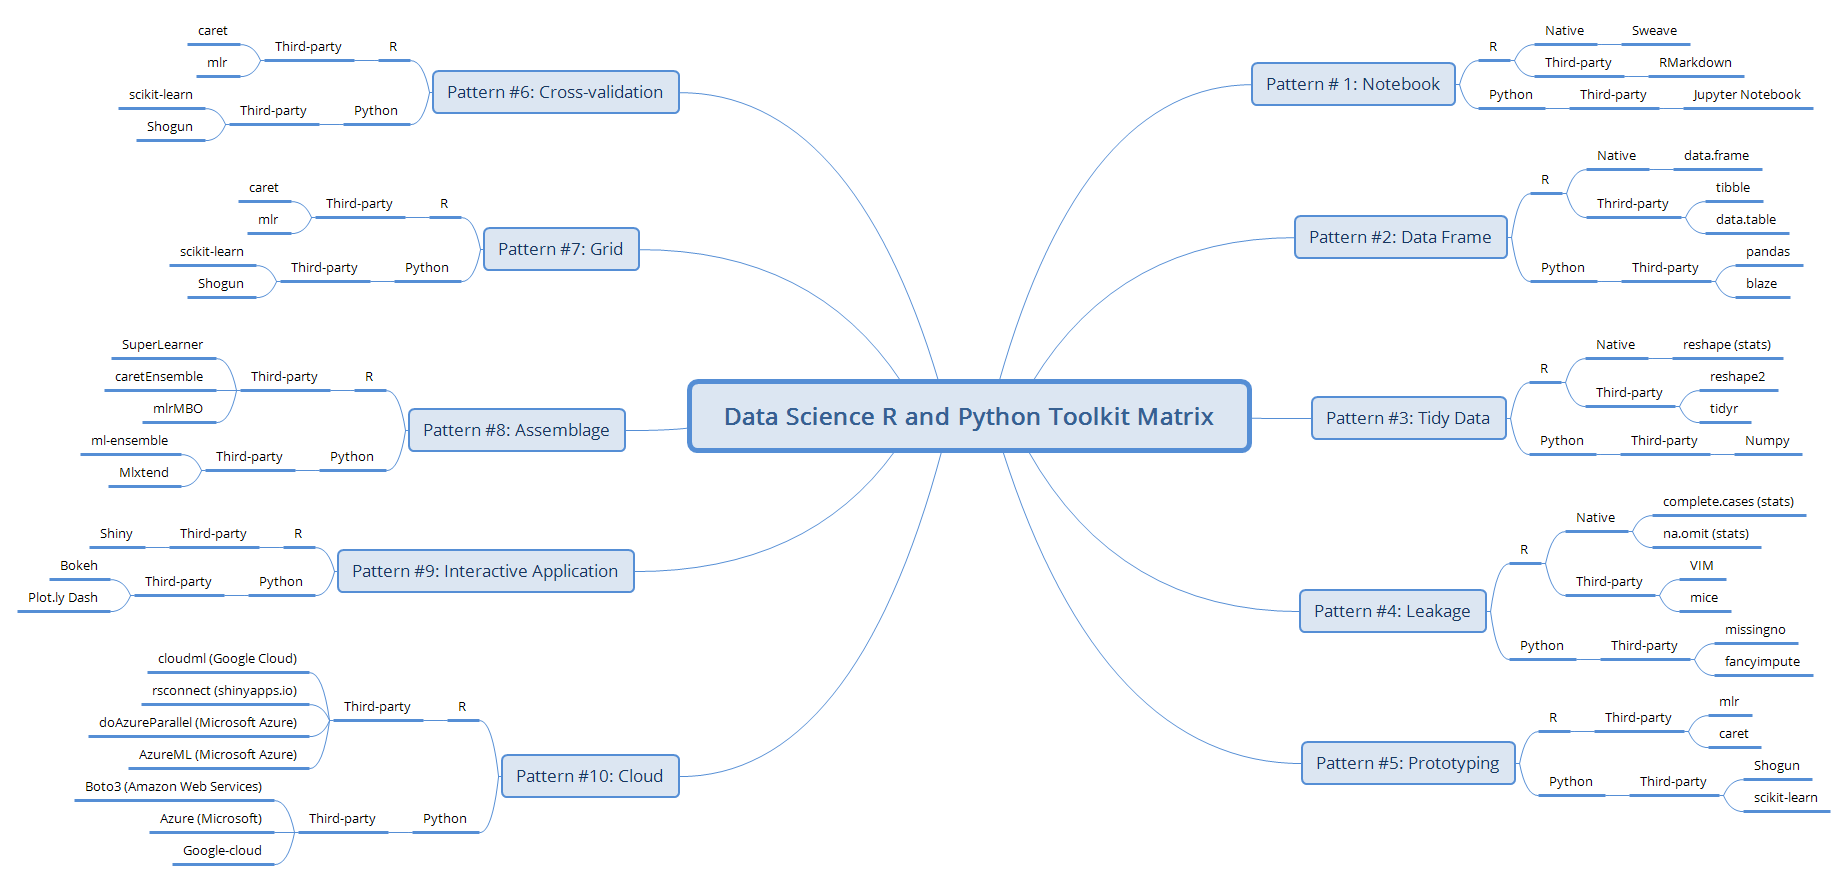
\includegraphics[width=\textwidth,height=\textheight,scale=0.9,keepaspectratio]{images/Data_Science_R_and_Python_Toolkit_Matrix.png}
\caption[Illustrates \acl{DSTM}.]{Illustrates \acl{DSTM} that consists of thirty-two packages and where applicable also with (R) native approaches that were incorporated into the language itself.}
\label{DTSMmindmapWithout}
\end{figure}
\end{landscape}




 \chapter{Reflection}
   \label{chap:summary}
   \lettrine[lines=2]{\color{BrickRed}T}{o} round up, this chapter discusses results of the endeavour taking into consideration various threats and limitations that arose during the examination. 
Moreover, with a perspective on future research, implications for scientists and practitioners are stated too.

%%%%%%%%%%%%%%%%%%%%%%%%%%%%%%%
\section{Discussion of Results}
\label{Discussion}
The research questions in this thesis led to formalizing ten data science design pattern candidates that were supplemented with source code examples and subsequently the identified packages were presented in the \acl{DSTM}.
In the following, a closer look is taken on both outcomes for the purposes of a discussion. 

\subsection{Design Patterns}
\marginnote{Pattern Language}
While each pattern was described relatively independently, as \textcite[10]{Fowler2002} has remarked, they should not be viewed \qcite{isolated from each other}. 
Accordingly and ideally, they form a basis for a \emph{pattern language} which helps stakeholders to utilize better \ac{DS} solutions and give programmers and other engineers the knowledge to \qcite{design complex systems} and processes \parencites[15]{DPSummarySMS2016}.
Specifically, ten patterns aid in creating a toolbox that data scientists not only need to be aware of but may actually actively use in their daily work when trying to make sense of data and produce conclusions for firm's target audience.  

Through pattern's backward and forward references, their associated network was shaped and visualized in Figure \ref{problem_solution_relationships} providing a \enquote{big picture} on a spectrum of related patterns targeting the same field \parencite{DeardenHCI2006}.
Correspondingly, what interconnects the examined group is the analytical engineering which is applied on data that are potentially of high value to the organization \parencites{GarrettGrolemund2017RData}{FosterProvost2013DataThinking}{Ayankoya2014}.
The information from literature sources has likewise indicated that while \ac{DS} patterns are likely unique due to conceivably useful (big) data, they are in many aspects similar to the ones described in the traditional software engineering \parencites{GoF2002}{GoogleDebt1}.
Essentially, both are dealing with the source code and sensible development practices for design and architecture of computer programs that perform specific tasks. 
However, what depicted patterns in this thesis have additionally focused on is the process by which data are managed, prepared and utilized for extracting a wisdom as such understanding forms an integral part of \ac{DS}.

In this study, the goal was not to develop a complete pattern language because of a very ambitious scope that would be necessary to consider. 
In fact, going back to the seminal publication of \textcite[394]{GoF2002}, authors have argued that there will be hardly \qcite{ever (\dots) a complete pattern language}. 
Therefore, theirs as well as the one of this work is \qcite{just a collection} and a family of accompanying problem and solutions pairs -- a catalogue aiming to better understand the science of gaining insights \parencites[394]{GoF2002}{Schmidt:1996:SP:236156.236164}.

Indeed, the completeness is influenced by several criteria, including the target audience which in this case were primarily the aspiring data scientists. 
Especially for them, the number of introduced patterns may be substantially larger when compared with already experienced professionals.
Therefore, in order to develop a complete design pattern language, it would need to significantly expand the breath, aiming to cover the whole \ac{DS} life-cycle -- from business understanding to the final deployment as described by the \ac{CRISP-DM} framework in Figure \ref{fig6}.

As\marginnote{Allied Patterns} mentioned previously, the relationships between patterns are visualized in Figure \ref{problem_solution_relationships} and at the epicentre of ten design patterns are two fundamental \ac{DS} elements: \emph{data frames} which are used for storing and processing information and \ac{ML} \emph{prototypes} which enable to acquire knowledge by applying supervised and unsupervised learning methods.
Besides those examined in the \textbf{chapter \ref{chap:DSDP}}, additional four present other plausible and related candidates.
One instance is \emph{Data Robbery} where facts are acquired in an unauthorized way, for example through data scrapping. 
Alternatively, \ac{DS} repository has to be not only searchable, well organized and sufficiently documented but also preferably under the version control system allowing to record project's history and development. 
However, in accordance with forty-one literature sources, due to not considering them as the most significant in the \ac{DS} domain, they were omitted in this work's deliberation as it has been limited by the scope. 
Although only a set of ten patterns was formalized, the links between that describe a relationship such as \enquote{enhances} or \enquote{visualized in} make it possible to call them forming an incomplete \emph{pattern language} in the \ac{DS} context \parencite{DeardenHCI2006}.

\marginnote{Patterns Individually}
Going into more detail, as it was suggested by \textcite{DobleMeszaros1997}, a pair of a

\noindent\begin{minipage}{\linewidth}
\centering
\includegraphics[width=\textwidth+2cm,height=\textheight,keepaspectratio]{images/DS_DP_Relationships}
\captionof{figure}{Illustrates a relationship between ten DS design patterns categorized into three distinctly coloured layers.
Four other plausible patterns in an ellipse were not examined in this work.}\label{problem_solution_relationships}

\captionof{figure}{Illustrates summaries of ten design patterns, see \protect\path{Master_DS_DP.xlsx}.}
\includegraphics[width=\textwidth+2cm,height=\textheight,keepaspectratio]{images/DS_DP_problem_solution_summary}
\label{problem_solution_summary}
\end{minipage} 
problem and corresponding solution was aimed to be \emph{single-pass readable} and it was summarized in one sentence form in Figure \ref{problem_solution_summary}.
Even though patterns were numbered, they should not be looked at to be in a specific order of use when compared to the ones by \textcite{Alexander1977}. 
Typically, for instance, data scientists may opt to utilize \patternName{Notebook} at the very end of the modelling process when they are required to present their results and enlighten stakeholders about achieved predictions and insights. 

The pattern language began first with a tool that permits data scientists to document their acquired knowledge using a consistent and simple format for description. 
An additional advantage of \patternName{Notebook} is that when text and code snippets are executed, the input and the output of the journal is rendered in line, making it cohesive within one file. 
Therefore, not only putting a focus on the right information being conveyed to business leaders but allowing to document the whole \ac{DS} as it has been pursued too. 

The visualization and communication of outcomes is critical and developing \patternName{Interactive Applications} that tell engaging stories and let to dive deeper into the data by adjusting how graphics look like only supports managers in outlining a strategy of how to increase the value of the products and services offered. 
Subsequently, the \patternName{Cloud} comes on the stage when created applications need to be deployed and scaled up and down to possibly thousands of employees worldwide whereby leveraging the resources and other features of cloud vendors. 
Thus, avoiding managing own hardware infrastructure as it likely not a core competency of the company.

Continuing, at the core of the knowledge discovery are naturally data, and therefore it is necessary to store them efficiently so that they can be manipulated and various mainly statistical operations can be carried out.
After accessing them from source systems, another pattern forms a foundation through creating a two-dimensional data structure in a tabular form. 
Consequently, the use of \patternName{Data Frames} enables to transform (\patternName{Tidy}) them with an objective to further simplify processing and their use within the targeted ecosystem of tools. 
Exemplary for \patternName{Prototyping} purposes, the outcome of which shall be impactful and reliable predictions for co-workers.

The \patternName{Leakage} is often consequential when modelling algorithms need to be applied because it can lead to conclusions which are statistically skewed and invalid, making them almost certainly not accurately reflecting the data at hand. 
In fact, missing data should be a prime source of a concern for any \ac{KDD} professional and due to their impact, missingness needs to be dealt with early on during the information pre-processing.
On the other hand, \patternName{Assemblage} and \patternName{Grid} leverage computing resources to optimize hyperparameters of each model as well as to create several ones and intelligently combine them to additionally improve the performance for stated aims and avoid overfitting where the \ac{ML} prototype is not generalizable to the new input.  
Undoubtedly, to validate the power of such model, \patternName{Cross-Validation} is \emph{the} technique to split data and calculating multiple predictions and test set errors on different data sets. 
As a consequence, average them to provide final unbiased outlook on the prototype.

Going back to section \ref{ds_dp_related_research} on the pattern related research, not surprisingly some of the design patterns identified in this thesis have been formalized and proposed by several researchers as well. 
Notably, the work of \textcite{HeffreMheer2006} is compelling as it describes for instance \patternName{Data Column} which is directly associated in this work to \patternName{Data Frames} by not only allowing to store data in a common format but permitting to administer various expressions on data themselves too -- what the same authors have described in a separate pattern called \patternName{Expression}.
Moreover, \patternName{Interactive Application} make it easy for users to dynamically change graphics, illustratively through filtering. 
On this matter, \textcite[859]{HeffreMheer2006} have described \patternName{Dynamic Query Binding} which automatically \qcite{refine[s] a data view through direct manipulation}.

\marginnote{Categorization}
Besides, it could have been observed that with an exception of \patternName{Notebook Design Pattern} all are mainly applicable to \ac{CRISP-DM} stages of data understanding, preparation, modelling, evaluation and deployment. 
Unfortunately, due to a delimitation of providing R and Python code examples, it was largely avoided to examine patterns related to the business understanding even though a considerable amount of information was collected.
Nonetheless, with regard to their grouping, patterns might be not only associated with specific \ac{CRISP-DM} phases as illustrated in Figure \ref{secondDatabaseExcel} but due to addressing different design \enquote{levels} they could be divided into three structural layers too \parencites{DeardenHCI2006}{ChenHong2004}:
%
\begin{enumerate}
	\item [(a)] \emph{Data Patterns}: \patternName{Data Frame}, \patternName{Tidy Data} and \patternName{Leakage}
	\item [(b)] \emph{Modelling Patterns}: \patternName{Prototyping}, \patternName{Cross-validation}, \patternName{Grid} and \patternName{Assemblage}
	\item [(c)] \emph{Infrastructure Patterns}: \patternName{Notebook}, \patternName{Interactive Application} and \patternName{Cloud}
\end{enumerate}

Principally, \emph{data patterns} consistently fetch, store and prepare analysis-ready information which is the primary object dealt with in \ac{DS}. 
Next, \emph{modelling patterns} take advantage of the previous group and enable to stepwise acquire better predictive models and with them previously not known wisdom.
At last, \emph{infrastructure patterns} support previous two categories by offering underlying tools that allow to deliver actionable insights, for example by developing on and deploying solutions to the cloud-based production systems.

As such, the above-mentioned three classes form a cohesive pattern language, in the \ac{DS} context, where its composition and interrelationships shall make it easier to derive, create and use best approaches to frequent hurdles in the knowledge discovery.

\subsection{Toolkit Matrix}
The third study question of this research has asked which open source tools are available in order to solve common pitfalls that each pattern has outlined and attempted to iron out. 
As a result of this inquiry and the conducted qualitative survey where thirty-two packages were sampled, \acl{DSTM} was visualized in Figure \ref{DTSMmindmapWithout}. 
This likely represents a valuable resource for researchers and practitioners because it can support them with gaining an overview of some of the essential applications for specific \ac{DS} tasks.
Particularly, when they might not be aware of them due to being new to the domain and coming from other languages.

While\marginnote{Sub-ecosystems} \textbf{chapter \ref{chap:KeyTerms}} has discussed R and Python software ecosystem from rather a high-level perspective, the outcomes presented through \ac{DSTM} also provide an extended and deeper perspective into available tools.
In fact, during the course of \ac{DS} pattern discovery, it was observed that five packages are a part of two collections that form sub-ecosystems in both programming environments, namely the previously mentioned R's \emph{tidyverse}\footnote{\href{https://www.tidyverse.org}{https://www.tidyverse.org/ -- Tidyverse}} (\mintinline{R}/tibble/ and \mintinline{R}/tidyr/) and Python's \emph{SciPy}\footnote{\href{https://www.scipy.org/}{https://www.scipy.org/ -- SciPy}} (\mintinline{python}/pandas/, \mintinline{python}/Jupyter/ and \mintinline{python}/Numpy/).

These sub-ecosystems, to which academicians have devoted so far only limited attention, provide utilities for \ac{DS} with an objective to simplify importing, processing, modelling and visualizing raw information. 
At the same time, individual libraries available on \ac{CRAN}, \ac{PyPI} or currently in the development for instance on \emph{GitHub} are strongly interlinked with each other by possessing typical ecosystem characteristics.
Namely, in pursuing a common philosophy around \ac{API} design and having a consistent implementation of internal components due to adopting specific conventions that allow to \qcite{guess how another different component} might work \parencite[785]{Bryan2017DataTent}.
Building upon interoperability within the respective universe of different packages sharing common objectives, group of developers and related infrastructure, two \qcite{cohesive system[s]} were created examined next \parencite[785]{Bryan2017DataTent}. 

Because\marginnote{SciPy} Python was developed as a general-purpose language and not being used for \ac{DS} intentions alone, it has aimed to offer fundamental concepts for many plausible use cases, in diverse areas including web development.
Therefore, the community of users had to build capabilities for \ac{DS} from the ground up as they were not present in Python itself and hence SciPy ecosystem was set up by a reason of lacking an efficient array manipulation or plotting of graphics \parencite{Millman2011PythonEngineers}.
Subsequently, due to the rise of its popularity, over the years it has become a gateway to \qcite{open-source software for mathematics, science, and engineering} -- the scientific computing -- for which it has developed a comprehensive knowledge discovery toolkit \parencites{Perez2011Python:Computing}{Oliphant2007}. 
On the other hand, tidyverse came from a different perspective as the community around R -- given its a priory focus on the analytical domain -- already had a blueprint on top of which it could build the improvements.

As mentioned\marginnote{Tidyverse} previously in section \ref{secos}, R has been in the development since 1993 and even earlier when considering its predecessor S. 
Ever since it has tried to be correct first, fast second and maintain backwards compatibility with tools being created back in the 1980s and 1990s \parencite{BlasMartinSlow2018}.
Resulting from this, however, is that many of the past choices in terms of what would a developer expect from a specific function may seem nowadays rather cumbersome to handle -- likewise called \qcite{historical inefficiencies and idiosyncrasies} by \textcite{RossZ2017DeclutterTools}. 
A typical example is R's native \mintinline{R}/data.frame()/ where by default any strings are silently converted to data type factor, which represents categorical variables, unless  provided with \mintinline{R}/stringsAsFactors = FALSE/ parameter \parencite{PengStringFactor2015}. 
While it may be a desired behaviour in many contexts, in others it causes a confusion, specifically for newcomers judged by a number of questions on websites like \emph{Stack Overflow} \parencite{WinVektro2014}. 
When compared to Python, this overcame similar challenges by introducing a completely new version 3.x as described in the \textbf{chapter \ref{chap:KeyTerms}}.

For R, where the innovation happening these days mostly in the package universe, tidyverse reimagines its already existing features in a new way by providing a consistent approach in \qcite{function syntax[, its arguments,] inputs and outputs}, thus \qcite{allow[ing] data analyses to flow naturally from one task to the next}, for instance through the \enquote{\%>\%} pipe operator while benefiting from data being in the \patternName{Tidy} format \parencite[2-3]{RossZ2017DeclutterTools}.
By contributing feature rich improvements that cannot be easily incorporated into the languages itself by reason of its heritage, it has been often taught from the beginning in the courses of statistics and \ac{DS} due to supporting \qcite{entire end-to-end workflow} \parencites{KellyPosterUSerRBrussels2017}{Rickert2017}.

Going back to the \ac{DSTM}, together with two sub-ecosystems, it has shown that users can clearly take advantages of such (and not limited to) participated packages because they are extensively documented and supported by a large and strong community of developers around them. 
Hence, helping to overcome any potential challenges faced by the users and at the same time ensuring that there is a seamless integration and compatibility beyond the both sub-ecosystems.

In general, three remarks could be made.
For one, some packages like \mintinline{python}/pandas/ and \mintinline{R}/mlr/ are in fact universal and can be used for multiple \ac{DS} design patterns, see Figure \ref{secondDatabaseExcel} where it was attempted to link and categorize libraries with \ac{CRISP-DM} framework and its six phases.
Indeed, these tools are not only suited of being used with their primarily associations (\patternName{Data Frame} and \patternName{Prototyping}) but with other relevant ones as well, including \patternName{Tidy Data}, \patternName{Grid} or \patternName{Cross-validation}.
As a result, beginners and experienced professionals should seek such comprehensive applications as they cover a wide range of tasks and permit to avoid jumping between different libraries that may not interact with each other in a simple manner.

Moreover, even though R's package ecosystem is approximately a tenth the size of Python's, it has shown to provide a richer set of \ac{DS}-related capabilities for diverse \ac{KDD} steps -- especially when omitting \emph{Usage Metrics} and \emph{Maintenance} criteria explained in Table \ref{tab:creteriaIncExcl}.
Nonetheless, both programming languages offer a large collection of \ac{DS} utilities, with and without previously mentioned two sub-ecosystems.
Given that Python's core developers have aimed to build a language that is applicable in a broader \ac{IT} landscape rather than just focusing on one particular area such as data analytics, \emph{R Core Team} could independently pursue a path of developing an open source alternative to \emph{Matlab} or \emph{Wolfram Language} that supports primarily mathematicians.
Thus, based on the gathered observations in the course of this thesis, the discussion of choosing between R and Python proves to be inappropriate as clearly R is more advanced for the data analysis, though it also offers little flexibility outside of its domain compared to Python and its ecosystem. 
Accordingly, the need to learn both of them, one after another, as explained by \textcites{MartijnTheuwissen2015R}{Theuwissen2016}. 

Finally, while recording tools in the database and creating \ac{DSTM}, the significance of \emph{GitHub} was manifested as being \emph{the} platform for the development and programmers' collaboration. 
Albeit arguably more feature rich alternatives like \emph{GitLab} or \emph{BitBucket} exist, all sampled packages have source code repository there and with a few exceptions make use (though to various degrees) of continues integration and deployment whereby software applications are automatically tested, build and released -- in line with Agile practises \parencites{BinasGitLab2013}{PaulGitlab2016}{AgileCI2009}.
As such, data scientists may use \emph{GitHub} not only for monitoring team's \ac{DS} progress, developing new packages and sharing publicly the result of data analysis with the source code but when discovering new projects currently in the development too.

\section{Limitations and Implications}
\label{ImplicationsLimitations}
The\marginnote{Repercussions} findings presented in this thesis add to the overall understanding of design patterns within the \ac{DS} field -- specifically where and how they can be applied to help distinct groups of stakeholders simplifying knowledge extraction from the diversity of data compiled.
The implications of this examination are important for both researchers and practitioners.

Firstly\marginnote{Scientists}, the contribution of this study was by providing a systematic review of extant research done in the fields of \ac{SECO}, \ac{DS} and design pattern -- all of which were put into a relationship. 
This served as a basis for a subsequent analysis and where missing elements were also identified such as very little studies dealing with Python software ecosystem and where more in depth investigations can be worthwhile. 
Additionally, the background research presented a solid evidence base for future inquiries as design patterns for \ac{DS} were not yet constructed and to what this study has finally devoted an attention, attempted to fill the gap and added to the body of research by extending the knowledge of design patterns which may be applied in a new interdisciplinary domain.
All this is particularly relevant for the community of scientists who might deliberate and discuss these ten design patterns and use deliverables to formulate new ones based on the already conducted exploration \parencite{Stol:2010:CUO:1833272.1833276}.

Although\marginnote{Professionals} any outcomes should be interpreted with caution, they give additional insights to various groups of stakeholders working directly with \ac{DS} teams as well as aspiring data scientists themselves. 
For the target audience of this thesis, the formalized patterns help to better understand what best practises could be leveraged when conducting \ac{DS} as they relate to problems that often come up and need to be tackled. 
Hence, pattern candidates shall educate and train for possible situations including in the modelling phase and case of overfitting and accordingly provide ideas and steps that may appropriately address them to minimize any negative impact. 
For experienced professionals, this work can further strengthen their expertise by (re)discovering practises and applications that they have not used so far, and thus equip them better for future occurrences and needs too.

Even though executives and \ac{UI/UX} designers might not be interested in technical details of data mining and \ac{KDD}, they can use these outcomes to become acquainted with some core principles behind the science of data as well. 
In fact, non-technically skilled managers should benefit from this information while navigating their organizations towards greater \ac{DS} adoption and utilization. 
As a result, they can prepare for potential challenges which it brings, for instance in terms of proper project management and data governance. 

Previously, it was mentioned that R and Python have two large sub-ecosystems of tools that provide well-established capabilities for \ac{DS}. 
Through explored applications that support each pattern candidate, \ac{DSTM} has the potential to give valuable guidelines for new (data science-oriented) programming languages such as \emph{Julia} too. 
This in understanding of what kind of tasks it needs to be able to address, for example by offering advanced modelling capabilities within a modular \ac{API}, in order to establish itself as \emph{the} language for \ac{KDD} purposes \parencite{Krishnakumar2011}.
Therefore, it helps a wide group of stakeholders, including vendors, individual developers, investors, and other contributors, to decide in which software ecosystem to invest their time, skills and other resources \parencite{Hoving2013Python:Ecosystem}

This\marginnote{Constrains} study, by discovering data science design pattern candidates, has established a starting point on which future research can base its findings.
Though, in the following, it is necessary to judge the conducted qualitative research as this thesis was subject to several conceptual and methodological weaknesses. 
When these limitations are explored and devoted a renewed attention by scientists, it could additionally help to increase pattern language's quality.
Indeed, in every step as documented in Figure \ref{figmmDesign}, unavoidable subjective choices were made which resulted into bringing a source of uncertainty on the outcomes. 
To compensate for taken decisions, it was attempted to explain the situation and provide a broader perspective on the matter \parencite{PetrovAarhus16}.

\textcite{Golafshani2003} has documented that depending on the type of study, authors had diverse views on what specific criteria should be of a concern in order to determine the quality of the research \parencite{Long2000RigourResearch}.
Some scientists have claimed that credibility, trustworthiness and rigour are suitable lenses and of a paramount importance in the qualitative and quantitative research alike -- all of which stem from the universally accepted terms of \emph{reliability} and \emph{validity} \parencites{Golafshani2003}{Long2000RigourResearch}. 
With regard to the former one, because of a difficulty in demonstrating it, a revision has been made to capture dependability and consistency \parencite{Golafshani2003}.
On the other hand, validity has been explained as to whether the study \qcite{represents accurately those features (\dots) that it is intended to describe (\dots) or theorize} \parencite[31]{Long2000RigourResearch}.
Coming next, some of the issues divided into three major categories are discussed.

\paragraph*{Construct and Internal Validity}
While construct validity deals with threats that \qcite{might arise during research design}, the internal validity investigates problems \qcite{during [the subsequent] data extraction} \parencite[13]{GoFDesignPatternsAmpatzoglou2013}. 

As noted by many researchers, being limited to the availability of data from which one may derive design patterns, the quality of selected literature sources is critically important. 
Overall, the work has shown to be able to derive ten candidates from a set of literature sources as opposed to directly for example interviewing domain experts.
Although more qualitative and quantitative data could have been gathered, the outcomes might not have changed much as ultimately a decision was taken to formalize only an initial subset of ten design patterns. 
On the one hand, the advantage of the approach described in section \ref{pprospecting} was that fewer restrictions and assumptions were placed on the research and on any data collected. 
Hence, allowing to assemble a reasonable sample according to the best efforts \parencites{Krishnakumar2011}{JAN:JAN623}.
At the same time, the study benefited from not only searching manually but also utilizing snowballing technique where additional resources were collected in order to support patterns' reliability.
On the other hand, the process is not fully reproducible and it could be argued that because it depended on information sources some of which were later deemed unreliable, it similarly lacks further power to be representative of the field too \parencite{Hajimia2014}.

While borrowing principles of \ac{SLR}, the search has been initially done through key words that were deemed appropriate by author's best judgement. 
Yet, due to a general paucity of the relevant primary and secondary data, the search was extended on several occasions by incorporating various new terms such as \enquote{lessons learned} to raise the quality and volume of gathered literature.
Later, the \ac{GIA} was applied to extract phrases and concepts that would lead to the discoverability of \ac{DS} pattern candidates.
Though, it should be noted here that text labelling was not supported by an independent parallel review of the same documents by other researchers as otherwise it would gain an additional trustworthiness by possibly clarifying misinterpretations and conducting \qcite{peer debriefings and stakeholder checks} \parencite[243]{t06}.
To increase such validity, a cautionary opinion of a fellow researcher could bring a novel angle to the most important design patterns in the \ac{DS} that shall be elucidated.

With regard to the toolkit matrix, even though it was attempted to discover relevant tools through criteria listed in Table \ref{tab:creteriaIncExcl}, author's a prior knowledge and any R and Python experiences might have negatively influenced the choice of tools too. 
This both in terms of their volume and relevancy, resulting into introducing selection and other cognitive biases into this work. 
As a consequence, unintentionally omitting applications that are of a great significance for the particular problem.

\paragraph*{Transferability}
Likewise called \emph{external validity}, transferability deals with \qcite{generalizing the obtained results from the sample to the population} \parencite[13]{GoFDesignPatternsAmpatzoglou2013}.

Naturally, patterns shall be neutral and easily applicable to other related areas, environments or technical applications.  
In the context of this research, it could be reasonably stated that described design patterns are not specific to the \ac{DS} per se because of their broad nature that covers a wide domain of business analytics and its engineering practises which are underpinned by the \ac{KDD} process.
Not surprisingly, given that \ac{DS} was defined as an umbrella term that covers a multitude of concepts, one may also find illustrated pairs of a problem and solution to exist in areas like \ac{ML} (\patternName{Grid} or \patternName{Cross-Validation}) or big data (\patternName{Cloud}). 
As stated previously, \emph{data frames} are typically used for a variety of use cases across the fields. 

Going back to \textcite{GoF2002}, authors have described design patterns with C++ examples. 
However, the notion of particular issue and answer to it can and has been applied in other languages, exemplary Java or Ruby as well \parencites{OrelyJavaDP2009}{RubyDP2007}. 
Thus, patterns in this research might have been supplemented with other programming languages, \emph{Matlab} to name one example.
Nonetheless, usually with modifications as presented artefacts in a predefined form are just templates which have to be adjusted due to a variety of faced situations or technologies \parencite{Fowler2002}.

\paragraph*{Confirmability}
As mentioned in section \ref{patternWritEvalu}, not only candidates were outlined based on the data from the gathered literature but through additional search of their practical application it was ensured that they are indeed being used at various stages of \ac{KDD} life-cycle and by data scientists themselves. 
Yet despite following \ac{3D2P} methodology, a triangulation of multiple methods for data collection, analysis and evaluation could potentially derive better findings and improve their confirmability. 

Indeed,\marginnote{Domain Experts} further research might repeat this work by meaningfully integrating other approaches used for pattern discovery. 
Along those listed by \textcite{InventadoPeter2015}, the knowledge of domain experts shared through in-depth interviews or writing workshops could plausibly prove to be the most relevant and valuable to have.
Hence, increasing the obtained wisdom both in the volume as well as mainly in its quality -- stemming from direct involvement of experienced professionals who were not, unfortunately, surveyed in the study.
Accordingly, help these design pattern candidates to acquire a more confidential status in order to spread farther their use within the community of data scientists and beyond.

\subsection{Future Research}
\label{futResearch}
In the future studies, among others, two notable paths can be pursued to establish a more complete \ac{DS} pattern language.

As it\marginnote{Different Approach} was noted, a research limitation of this study is utilizing literature works rather than interviewing experts from the domain who could likely outline problems and solutions that they apply in a more reliable fashion. 
Consequently, based already on the conducted research, the next step would be to try to empirically confirm findings and thus enhance the quality of identified design patterns for example though a quantitative survey of \ac{DS} experts from diverse industries and countries.
Furthermore, if a choice had been made to use mixed methods methodology, expert interviews could have been combined with a literature review leading to supposedly further increasing the value of formalized design patterns.

Moreover\marginnote{Different Perspectives}, being limited by practical constraints, the thesis could not provide a comprehensive review of the whole \ac{DS} landscape. 
This is a reason a decision was taken to describe only a number of pattern candidates linked to the domain. 
However, during the stages of \emph{pattern prospecting} and \emph{pattern mining} large amounts of various information were gathered and this may be used to uncover and formalize new problem and solution pairs. 
In fact, it was observed that some plausible patterns are related not only to \emph{technical} aspects (and on which this study has tried to zoom in) but also to the \emph{organizations} or the \emph{environment} -- in line with TOE framework, firm's contexts and forces influencing the adoption of any kind of technology \parencites{BakerTOE2012}{tornatzky1990processes}{OlivertraTOE2011}.
As a result, additional pattern examples ought to include themes like how to acquire stakeholders' support for \ac{DS} initiatives, how to tackle right analytical problems in right way that encourages their involvement and how to convert and educate business analysts to become data scientists \parencites{Fern2016}{SAS2016}{CarlShan2015TheScientists}.  
Therefore, extra research shall examine more closely collected data, seen in Figure \ref{fit-excel-database-sourcedata}, from different perspectives and attempt to discover other design patterns when considering the whole life-cycle of \ac{DS}. 

At the\marginnote{Entanglement} high-level of perspective, data science design pattern may ease the complexity of interaction between \emph{technical} systems (like R and Python which simplify conducting specific tasks) and \emph{social} ones where humans participate in some organizational structure and use the technology to accomplish their goals \parencites{WandaSusan2008}{BrianSTS2009}.
At the core of this \emph{socio-technical system} theory is the idea that a process such as data analysis has to take into account not only technical factors that influence the functionality, usage and a wisdom gained from applying \ac{DS} but a whole set of interdependent social aspects too which cannot be treated as separate parts in a complex system \parencite{BaxterST2011}.
However, in this thesis the focus was only on the technological domain that cannot be viewed independently due to  complex linkages and mutual interactions between design patterns themselves and a developer who has to shape and adjust these templates \parencite{Fowler2002}. 
Thus, in the future research it could be interesting for example to formulate \ac{DS} design patterns as seen from the social angle and considering expanding the above-mentioned TOE framework with a socially based individual dimension \parencite{PetrovAarhus16}. 
Exemplary, make an inquiry of how identified patterns are applied differently, though being in similar circumstances.
The reason for this might be the impact stemming from various organizational and individual aspects, from the cultural influence to Hofstede's power distance between employees \parencites{Holfstede1993}{Holfestede2011}.

Besides\marginnote{Multidimensionality}, going back to section on delimitations of this work, further studies  extending design pattern by presenting corresponding anti-patterns would be very interesting as well.
Additionally, with recent advancements in the artificial intelligence it is clear that one will need to explore applications that support multidimensional data and associated patterns which this thesis has intentionally omitted when it was focusing only on the tabular ones. 
Illustratively, the work of \textcite{PerezBook2017} already attempts to put an attention on the concept of \emph{deep learning} and design patterns that can be practically applied in the robotics or self-driving vehicles.

To summarize, what has been described in the \textbf{previous chapter} helps data scientists to become better equipped with technical and theoretical knowledge of processing data stored in various quality and granularity when producing business relevant, actionable results to themselves and other internal and external co-workers.
At the same time, novel studies in the area of design patterns for analytical purposes shall not only use gathered data in Figure \ref{fit-excel-database-sourcedata} to develop new candidates but also try to qualitatively validate those described in this thesis for instance though expert interviews. 
Indeed, when this and other supplementary research is pursued and conducted, it can foster effective management of company's expectations in relation to the broader and inseparable \qcite{technology, techniques, and people} \parencite[68]{Bhatt2001}.

%%%%%%%%%%%%%%%%
\section{Conclusion}
\label{Conclusion}
To conclude, given the scarcity of information in the current literature regarding \emph{data science design patterns}, the quest of this work was to address this lack by exploring and describing their first, known to the author, systematic account. 
As a result, the inquiry has tackled frequently arising problems and their best solutions in the interdisciplinary field of \ac{DS}.
Essentially, the goal was to qualitatively note a \qcite{common solution, look for its core, and then write down the resulting pattern} \parencites[10]{Fowler2002}{Schmidt:1996:SP:236156.236164}.

Focusing on \ac{DS} design patterns, a devised research gap led to formulating the main objective of uncovering solutions to identified issues and secondary aim of supplementing drafted artefacts with practical examples using utilities from R and Python ecosystem.
Subsequently, this translated into three study questions, the first of which was to understand key terms.

As such, the work began with an exploration of software ecosystems of R and Python.
Characterized by different actors, though appearing and collaborating as a group on the same technological platform, these were later surveyed in order to identify libraries and provide source code examples to each design pattern. 
Certainly, both environments offer a wide range of applications supporting researchers and practitioners in analysing data in different disciplines, with R having an edge by reason of its rather domain-specific focus. 
While two programming languages are also distinct, they share a large, often interacting, community of users and developers who participate in their common aspirations -- be it for advancing the analysis and visualization of data or for development of web applications and system-level scripting. 

Although \ac{DS} may not have been a novelty because of absorbing other existing concepts like \ac{ML} and big data, section \ref{termsDef} explained that it has become associated with loosely defined analytics where not only sound mathematical foundations are necessary but software engineering experience too.
By cause of a diversity of conducted tasks, data scientists have been needed who combine a multitude of critical skills in their work such as the proficiency in statistics, deep domain know-how and among others the ability of programming with R and Python. 
Even though the field may have roots in the academia and research where different information has always been analysed, skilled data scientists are these days difficult to identify and come by.
Therefore, for example, if business analysts want to advance their career and move into more technical field, the presented \ac{DS} design patterns may benefit them by gaining an initial understanding of best practises that can solve common issues when acquiring insightful knowledge. 

After key phrases were reviewed in detail, a research methodology was presented in the \textbf{chapter \ref{chap:Method}} incorporating qualitative methods under the stewardship of the \emph{data-driven design pattern production} framework.
By using a systematic \ac{GIA} for gathered data, major themes were mined from a final set of forty-one literature sources -- all that in order to discover and formulate yet-to-be-verified design pattern candidates.
As a result, based on the understandings of three concepts, the illustrated methodology helped to systematically accumulate data, analyse them and codify these patterns in a simple to understand template form.
Unfortunately, while many potential candidates could have been found dealing for instance with data normalization, it was beyond the scope of this work to describe them all in a complete language.  
Not coincidently where more research remains to be pursued as there is no silver bullet to work out each encountered problem.
Hence, only a set of ten pieces was elucidated together with gaining a larger picture into R and Python ecosystems and how they can solve arising \ac{DS} issues. 

Overall, the results of this thesis should help professionals in the \ac{DS} and associated fields to more easily document and share their wisdom and best practises through used vocabulary and benefiting from a specific form that was applied for their formalization. 
As discussed earlier, the artefacts could be categorized into three groups according to the primary subject matter being dealt with, namely data, \ac{ML} prototype or infrastructure. 
Therefore, this classification shall further aid in decomposing \ac{DS} problems into manageable parts and offer a matching tool for avoiding \qcite{wasting time and resources reinventing the wheel} both in terms of creating new duplicate tools as well as questionable, yet-to-be-verified approaches to a particular \ac{DS} problem \parencite[20]{FosterProvost2013DataThinking}.  

When equipping ten design patterns in the \textbf{chapter \ref{chap:DSDP}} with a collected sample of thirty-two R and Python packages, some libraries were used for displaying source code examples too. 
In this manner, supporting target audience in showing a reliable set of tools capable of addressing outlined issues that occur when following a process methodology such as \ac{CRISP-DM}.
Within the sample, five tools were also identified stemming from two R and Python sub-ecosystems, named tidyverse and SciPy.
Documented in \textbf{this chapter}, these aim at providing a complete end-to-end toolbox that might be beneficial for any emergent \ac{DS} purpose and use cases, from managing (big) data using in-memory data frames to building predictive models that power business forecasts through applying comprehensive, well-known \ac{ML} libraries.

The collected utilities from two (sub-)ecosystems for each design pattern permit to answer the third study question whereby creating \acl{DSTM}. 
From this map, undoubtedly, newcomers to \ac{DS} can gain a starting point into R and Python environments by reason of visualizing some of the fundamental, arguably \enquote{most useful and popular}, tools like \mintinline{r}/caret/, \mintinline{python}/pandas/ or \mintinline{r}/Shiny/.
Subsequently, it can lead researchers and practitioners to utilize most appropriate applications for a particular situation that is being faced in their work.

Indeed, designing \ac{IT} architecture for analysing data requires significant human efforts whereby mistakes in the process are learned with the experience over a period of time. 
In order to avoid pitfalls, the knowledge of dedicated design patterns examined in this thesis, coupled with others like big data or cloud computing, can greatly simplify employees' working intentions and help to take educated decisions right from the beginning. 
Nonetheless, \textcite[13]{Fowler2002} writes that one should \qcite{never forget that [they are] a starting point, not a final destination}. 
Even though design patterns give a common ground to \qcite{communicate, document, and explore design alternatives}, it is always necessary to see them in the context of specific work assignments, usually within a constrained business structure and its available technology and resources \parencite[389]{GoF2002}.
Thus, when tackling \ac{DS} challenges, due to internal systems and processes, data complexity or surrounding organizational environment, ten design patterns will nearly always require further adjustments to a particular case, applications used and possibly developer experiences and preferences too.
As such, pattern candidates need to be thoroughly understood by practitioners before being applied.
Otherwise there is a risk of running into a situation where methods and solutions are exercised without fully realizing why they are needed, what is their impact and how they contribute to the acquisition of the wisdom in the first place. 

Overall, the described design patterns contribute in better understanding of how they can address and solve, together with source code examples that employ tools from R and Python software ecosystem, ten frequently arising \ac{DS} problems.
Almost certainly more research will be pursued, for instance by \textcite{Todd2019}, however, as the outlined aims from the introduction were achieved, a conclusion is made here.


\startappendices
\appendix{Figures}
\label{app:figures}
\begin{landscape}
\begin{figure}[ht]
\centering
\includegraphics[width=\textwidth+2cm,height=\textheight+2cm,keepaspectratio]{images/lit_database_progrLandscape}
\caption[Illustrates a literature database that is used for reviewing R and Python ecosystem.]{Illustrates a literature database that is used in section \ref{rpythonlandscape} to provide a review of corresponding articles where surveys of different programming ecosystems have been conducted, see \path{Master_DS_DP.xlsx}.}
\label{fig-literature-programLandscape}
\end{figure}
\end{landscape}

\begin{landscape}
\begin{figure}[ht]
\centering
\includegraphics[width=\textwidth+2cm,height=\textheight+2cm,keepaspectratio]{images/lit_database_surveyTools}
\caption[Illustrates a literature database that is used for inspecting studies which survey computer programs.]{Illustrates a literature database that is used in section \ref{surveyofTools} to provide a summary of articles surveying different software applications, see \path{Master_DS_DP.xlsx}.}
\label{fig-literature-database}
\end{figure}
\end{landscape}

\begin{landscape}
\begin{figure}[ht]
\centering
\includegraphics[width=\textwidth,height=\textheight,keepaspectratio]{images/DW_BI_System}
\caption[Illustrates a typical approach to building DW/BI system.]{The figure draws upon \textcites{WarrenThornthwaite2012MicrosoftApproach}{Kimball2008TheToolkit} and presents a typical architectural design of building data warehouse/business intelligence system, see \path{DW_BI_Structure.pdf}. 
Data are first extracted from the source systems such as (non-)relational databases or flat files (for instance comma-separated values documents) into the staging area. 
Then, they are transformed for building the \emph{dimension} and \emph{fact} tables. 
At last, they are loaded for example into data marts and \ac{OLAP} cubes in order to present them in the diverse \ac{BI} frond-end applications.}
\label{fig-bi-dw-schema}
\end{figure}
\end{landscape}

\begin{figure}[ht]
\centering
\includegraphics[width=\textwidth,height=\textheight,keepaspectratio]{images/CRISP-DM}
\caption[Illustrates six phases of CRISP-DM methodology.]{Illustrates six iterative phases of \acs{CRISP-DM} methodology and the prevalence of \emph{data strategy}, \emph{data science} and \emph{data engineering}. 
All this with regard to each \ac{CRISP-DM} stage where the portion of data strategy tries to bridge the gap between \emph{what} and \emph{why}. 
On the other hand, the part of data science combines business and technology skills for answering targeted questions, for instance through model building. 
Finally, data engineering works on the end-to-end analytical platform where data are acquired, later processed by means of \ac{ETL} pipeline and presented to stakeholders.
Inspired by \textcites{PeteChapman2004CRISP-DMGuide}{AnjaliSamani2016WorkingTeams}.}
\label{fig6}
\end{figure}

\begin{landscape}
\begin{figure}[ht]
\centering
\includegraphics[width=\textwidth+2cm,height=\textheight+3cm,keepaspectratio]{images/lit_database_ds_dp_studies}
\caption[Illustrates a literature database that is used for inspecting information resources related to design patterns.]{Illustrates a literature database that is used in section \ref{ds_dp_related_research}. 
It provides a short summary of articles and internet sources that were reviewed, see \path{Master_DS_DP.xlsx}.}
\label{fig-literature-database-ds-dp-research}
\end{figure}
\end{landscape}

\begin{landscape}
\begin{figure}[h]
   \centering
   \begin{tabular}{@{}c@{\hspace{.5cm}}c@{}}
       \includegraphics[page=1,width=.5\textwidth+1cm, height=\textheight+1cm,keepaspectratio]{images/Thesis_protocol} & 
       \includegraphics[page=2,width=.5\textwidth+1cm, height=\textheight+1cm,keepaspectratio]{images/Thesis_protocol} \\[.5cm]
	\end{tabular}
\caption[Illustrates a thesis protocol.]{Illustrates how does the thesis protocol look at the very end, see \path{Thesis_protocol.pdf}.}
\label{fig-database-research-protokol}
\end{figure}
\end{landscape}

\begin{landscape}
\begin{figure}[ht]
\centering
\includegraphics[width=\textwidth+2cm,height=\textheight+3cm,keepaspectratio]{images/excel_database_of_sources}
\caption[Illustrates an excerpt from a concept matrix that is used for discovering pattern candidates.]{Illustrates an excerpt from a concept matrix that is used for discovering \acs{DS} design pattern candidates in \textbf{chapter \ref{chap:DSDP}}. 
The full matrix is provided in the supplement, see \path{Master_DS_DP.xlsx}.}
\label{fit-excel-database-sourcedata}
\end{figure}
\end{landscape}

\begin{landscape}
\begin{figure}[ht]
\centering
\includegraphics[width=\textwidth,height=\textheight,keepaspectratio]{images/R_Python_Database}
\caption[Illustrates R and Python software tools that were used for design patterns.]{Illustrates seventeen R and fifteen Python software tools that were identified and some of which were used for design pattern code examples. 
Only two R packages (\mintinline{R}/cloudml/ and \mintinline{R}/doAzureParallel/) are as of \monthdataMyOwn\@ in development on \emph{GitHub}.
See the database in \path{Master_DS_DP.xlsx} as well.}
\label{fig11}
\end{figure}
\end{landscape}

\begin{landscape}
\begin{figure}[ht]
\centering
\includegraphics[width=\textwidth,height=\textheight,keepaspectratio]{images/DS_CRISP-DM_Matrix}
\caption[Illustrates links between design patterns, tools and stages of CRISP-DM framework.]{Illustrates links between formalized \ac{DS} design patterns, identified software tools and their association with stages of CRISP-DM framework, see \path{Master_DS_DP.xlsx}.}
\label{secondDatabaseExcel}
\end{figure}
\end{landscape}

\cleardoublepage


\appendix{Tables}
\label{app:tables}
\begin{landscape}
\begin{longtable}{|C{3cm} |C{3cm}| C{10cm} | C{2cm} | C{2cm} |}
    \caption[Presents steps by which information sources are collected and processed.]{Presents steps by which information sources are collected and processed. 
    For more, see the methodology in Figure \ref{figmmDesign} too.} \label{tab:creteriaIncExclDocuments} \\
    \hline
    \theadCenterText{Step} & \theadCenterText{Source} & \theadCenterText{Description} & \theadCenterText{Used for ...} & \theadCenterText{Total \# of resources} \\ \hline
    \endfirsthead
    \multicolumn{5}{|c|}{\tablename\ \thetable\ -- \emph{Continued from previous page}} \\
	\hline
    \theadCenterText{Step} & \theadCenterText{Source} & \theadCenterText{Description} & \theadCenterText{Used for ...} & \theadCenterText{Total \# of resources} \\ \hline
    \hline
    \endhead
    \hline
    \multicolumn{5}{r}{\emph{Continued on next page}} \\
    \endfoot
    \endlastfoot
    Keywords (initial search) & Scopus, Web of Science, Google (Scholar) & Material, including grey literature, where following keywords were found: \enquote{(best/good) approach(es)/advice(s)/practise(s)/
    solution(s)/recommendation(s)}, \enquote{data science/\ac{ML}/\ac{BI}/big data}, 
    \enquote{data analytics/analysis/mining}, \enquote{(abstract/common/frequent) problem(s)/mistake(s)}, \enquote{lesson(s) learned}, \enquote{(design) pattern(s)} & Inclusion & \multirow{2}{*}{26} \\ \cline{1-4}
    Practical Screen & \noindent\rule{1cm}{0.4pt} & Documents must have a clear purpose and addressing objectives of the study. & Exclusion & \\ \hline
    Snowballing & Sample of 26 resources & Additional information is collected by means of inspecting identified documents and extending an initial sample through iteratively snowballing  other studies. & Inclusion & 66 \\ \hline
    Quality assurance & Sample of 66 resources & A number of documents, which were classified as \enquote{poor} and \enquote{fair} on a four-step scale (very good, good, fair and poor), are excluded. & Exclusion & 41 \\ \hline
    \end{longtable}
\end{landscape}

\begin{landscape}
\begin{longtable}{|C{1cm} | C{3cm} | C{2.5cm} | C{11cm} | C{2cm} |}
    \caption[Presents criteria which are used for tool's inclusion and exclusion.]{Presents, in order of importance, criteria which are used for tool's inclusion and exclusion in the study.} \label{tab:creteriaIncExcl} \\
    \hline
    \theadCenterText{\#} & \theadCenterText{Criteria} & \theadCenterText{Type} & \theadCenterText{Description} & \theadCenterText{Used for ...} \\ \hline
    \endfirsthead
    \multicolumn{5}{|c|}{\tablename\ \thetable\ -- \emph{Continued from previous page}} \\
	\hline
    \theadCenterText{\#} & \theadCenterText{Criteria} & \theadCenterText{Type} & \theadCenterText{Description} & \theadCenterText{Used for ...} \\ \hline
    \hline
    \endhead
    \hline
    \multicolumn{5}{r}{\emph{Continued on next page}} \\
    \endfoot
    \endlastfoot
    1 & Release on \ac{CRAN} or \ac{PyPI} & Qualitative & At the point of survey, included packages should be released on either central repository -- hence being open sourced in nature. 
    If a package has not yet been published due to being in development, upon author's own discretion it might be considered as well. & Inclusion \\ \hline
    2 & Purpose & Qualitative & A package is excluded if it does not have a clear purpose and addressing the needs of each data science design pattern. & \multirow{3}{*}[-32mm]{Exclusion} \\ \cline{1-4}
    3 & Website & Qualitative & A package is excluded if it does not have a dedicated website (including a public source code repository) where users can find more information, for example  documentation. & \\ \cline{1-4}
    4 & Usage Metrics & Quantitative & A package is excluded if does not have a recognizable number of downloads or other metrics supporting being used in the community, made available for instance by \mintinline{html}{Rdocumentation.org}, \mintinline{html}{anaconda.org} or \mintinline{html}{Depsy.org}. & \\ \cline{1-4}
    5 & Maintenance & Quantitative & A package is excluded if it seems to be abandoned in terms of changes to the source code repository -- in fact it should have a publicly released version during a time period since January 2016 until \monthdataMyOwn\@. & \\ \hline
    \end{longtable}
\end{landscape}




% https://tex.stackexchange.com/a/112886
\startbibliography
 \begin{singlespace}
  \renewcommand*{\UrlFont}{\rmfamily}
  \printbibliography[title={REFERENCES}]
 \end{singlespace}

\end{document}
